\documentclass[a4paper,11pt]{report}
%FONT size can be changed on the above line
\usepackage[left=2.7cm,right=2.7cm,top=4cm,bottom=3.5cm,bindingoffset=0cm]{geometry}
%%% Headers
\usepackage{fancyhdr}
\renewcommand{\chaptermark}[1]{%
\markboth{#1}{}}  
\pagestyle{fancy}
\fancyhead[LO]{}
\fancyhead[RE]{}
\fancyhead[LE]{\textit{\leftmark}}
\setlength{\headheight}{15pt}

%%%%
\usepackage{tabularx}
\usepackage{amsmath}
\usepackage{amssymb}
\usepackage{ntheorem}
\usepackage{graphicx}
\usepackage{setspace}
\usepackage[outdir=./]{epstopdf}
\usepackage{caption}
\usepackage{subcaption}
\usepackage{array}
\usepackage{paralist} 
\usepackage{datetime}
\usepackage{verbatim}
\usepackage{makeidx}
\usepackage{titling}
\usepackage{titlepic}
\usepackage{enumitem}
\usepackage[toc,page]{appendix}
\usepackage[breaklinks=true]{hyperref}
\usepackage{pdfpages}
\usepackage{mathrsfs}
\usepackage{etaremune}
 \usepackage{bm}
\usepackage{sansmath}
\usepackage{pgfplots}
\usepackage{mdframed}
\usepackage{tikz}
\usepackage{float}
\usepackage{tikz-3dplot}
\usepackage{stmaryrd}
%%Fix line breaks for long citations
\usepackage{breakcites}
\usepackage{siunitx}
\usepackage{tocbibind}
\usepackage{lipsum}
\usepackage{minted}
\usepackage{caption}
\usepackage[list=true,listformat=simple]{subcaption}

\renewcommand{\epsilon}{\varepsilon}
\usepackage[style=ieee]{biblatex}

\addbibresource{references.bib}

\mdfdefinestyle{MyFrame}{%
%    linecolor=blue,
        linewidth=1pt,
%    roundcorner=20pt,
%    innertopmargin=\baselineskip,
%    innerbottommargin=\baselineskip,
%   innerrightmargin=20pt,
%    innerleftmargin=20pt,
%    backgroundcolor=gray!50!white
}
\usepackage{svg}
\usepackage{listings}
%New colors defined below
\definecolor{codegreen}{rgb}{0,0.4,0}
\definecolor{codegray}{rgb}{0.5,0.5,0.5}
\definecolor{codepurple}{rgb}{0.58,0,0.82}
\definecolor{backcolour}{rgb}{0.95,0.95,0.92}

\lstdefinestyle{mystyle}{
  backgroundcolor=\color{backcolour}, commentstyle=\color{codegreen},
  keywordstyle=\color{magenta},
  numberstyle=\tiny\color{codegray},
  stringstyle=\color{codepurple},
  basicstyle=\ttfamily\small,
  breakatwhitespace=false,         
  breaklines=true,                 
  captionpos=b,                    
  keepspaces=true,                 
  numbers=left,                    
  numbersep=5pt,                  
  showspaces=false,                
  showstringspaces=false,
  showtabs=false,                  
  tabsize=4
}
\lstset{style=mystyle,upquote=true}

\begin{document}


\begin{titlepage}
    \begin{center}

    \vspace{30pt}
    
\includegraphics[width=0.5\textwidth]{figures/ATULogo.png}\\
    \vspace{50pt}
    
    \fontsize{14}{20} \selectfont
    \setstretch{2.0}{\textbf{\Huge Automated Detection of COVID-19 using Convolutional Neural Networks and Generative Adversarial Networks}} 
    \vspace{20pt}
    
    A thesis submitted \\
    by\\
    \vspace{10pt}
    
    {\huge Ultan Kearns}\\
    \vspace{10pt}
    
     in partial fulfillment of the requirements for the degree of\\ Master of Science in Computing in Big Data Analytics and Artificial Intelligence
    \vspace{20pt}

%        \fontsize{16}{20} \selectfont
    
    
    Supervisor: Dr Paul Greaney
    \vspace{30pt}
    
    
Submitted to Quality and Qualifications Ireland (QQI) \\
Dearbhú Cáilíochta agus Cáilíochtaí Éireann
    \centerline{\monthname \quad \the\year}
\end{center}    
\end{titlepage}

\onehalfspace


\setcounter{page}{1}

\setcounter{tocdepth}{2}

\addtocontents{toc}{\protect\setcounter{tocdepth}{-1}}
\tableofcontents
\addtocontents{toc}{\protect\setcounter{tocdepth}{2}}
\chapter*{Declaration}
\addcontentsline{toc}{chapter}{Declaration}

I hereby certify that this material, which l now submit for assessment on the programme of study leading to the award of Master of Science in Computing in Big Data Analytics and Artificial Intelligence, is entirely my own work and has not been taken from the work of others except and to the extent that such work has been cited and acknowledged within the text of my own work. No portion of the work contained in this thesis has been submitted in support of an application for another degree or qualification to this or any other institution. I understand that it is my responsibility to ensure that I have adhered to LYIT’s rules and regulations. 
\bigskip

I hereby certify that the material on which I have relied on for the purpose of my assessment is not deemed as personal data under the GDPR Regulations. Personal data is any data from living people that can be identified. Any personal data used for the purpose of my assessment has been psuedonymised and the data set and identifiers are not held by LYIT. Alternatively, personal data has been anonymised in line with the Data Protection Commissioners Guidelines on Anonymisation.
\bigskip

I give consent for my work to be held for the purposes of education assistance to future Computing students at LYIT and it will not be shared outside the Department of Computing at LYIT. I understand that my assessment may be shared with any other third party and will be held securely in LYIT in line with the Institute's Records Retention Policy. 

\vspace{20pt}

\hspace{60pt} Signed: \underline{\quad \quad Ultan Kearns\hspace{240pt}} 


\bigskip

\hspace{70pt} Date: \underline{\quad \quad\today\hspace{150pt}} 
\chapter*{Acknowledgements}
\addcontentsline{toc}{chapter}{Acknowledgements}
I would first of all like to thank my supervisor during this project Dr. Paul Greaney, he was a fantastic help throughout the course of writing this thesis and this work could not have been completed without his input and help.
\\[1.5cm]
I would also like to thank the lecturers who taught me so much during my postgraduate course, both Doctors Karla Muñoz-Esqueival and Shagufta Henna provided a fantastic introduction into many areas of Artificial Intelligence and the knowledge they imparted has helped me a lot throughout the course of conducting this research. 
\\[1.5cm]
I would also like to thank Andrew Ng, his deep learning courses provided a great foundation into the realm of deep learning and Artificial Intelligence.
\\[1.5cm]
I would like to thank Francois Chollet whose book ``Deep Learning with Python`` was an indispensible resource and helped me get more familiar with the Keras library as well as the best AI practices and concepts such as transfer learning.
\\[1.5cm]
Finally I would like to thank my parents,and friends for supporting me throughout the course of this masters.

\chapter*{Acronyms}
\addcontentsline{toc}{chapter}{Acronyms}
\begin{table}[h]
    \centering
    \begin{tabular}{|c|c|}
        \hline
         Acronym
         &  Stands For\\
        \hline
        AI & Artificial Intelligence\\
        ANN & Artificial Neural Network\\
        CNN & Convolutional Neural Network\\
        GAN & Generative Adversarial Network\\
        CT & Computed Topography\\
        LSTM & Long short term memory\\
        AUC & Area under curve\\
        DCNN & Deep Convolutional Neural Network\\
        RCNN & Regions with CNN Features\\
        VAE & Varational Auto Encoder\\
        DCGAN & Deep Convolutional Generative Adversarial Network\\
        \hline
    \end{tabular}
    \caption{Acronyms used in this thesis}
    \label{tab:Table of Acronyms}

\end{table}
 


\listoffigures
\listoftables
\begin{abstract}
    This paper aims to analyze the applications of generative adversarial networks or GANs in overcoming issues of data-shortages in relation to developing convolutional neural networks to automate the diagnosis of COVID-19 in patients.  There have been many COVID-19 data-sets compiled but some suffer from lack of data-quality and data shortages\cite{covid19DataQuality}\cite{covid19DataQuality2}.  In this paper I aim to create and train multiple convolutional neural networks or CNNs to analyze X-Rays of patients lungs to automate the detection of COVID-19.  The CNN will be trained with a number of images generated from different GAN architectures to determine which will prove most efficient in automating the detection of COVID-19.  I also aim to use the GANs in conjunction with one and other to try out different combinations to see if feeding images generated by one GAN to other GANs will produce more accurate results when training the model.  In the results section of this Thesis I will compare and contrast the results of the various architectures and determine which proved most effective in it's diagnostic potential.
\end{abstract}

\chapter{Introduction}

\section{Explanation of Generative Adversarial Networks (GANs)}
A generative adversarial network or GAN for short first appeared in a 2014 paper by Ian Goodfellow et al\cite{generativeAdversarialNetworks}.  In this paper Goodfellow et al propose a new way to generate data via an adversarial process.  The GAN essentially works as follows: two models are trained, a generative model $G$ which will generate the synthetic data from the real data and another model $D$ which will be the discriminator, judging if the data was created by the model or if it came from the dataset.  The goal of this training is to ensure data generated from $G$ is realistic enough to make the discriminator $D$ believe that the generated content came from the training set, this is achieved by training the model for a number of epochs and adjusting the models weights to improve the quality of the generated image.  It  is in this way that we can create realistic "fake" data from the generative model.
\\
There are a number of GAN architectures which are useful in different scenarios, such as CycleGans\cite{cycleGan} which are useful for translating images from a source domain $X \rightarrow Y$ in which $Y$ is the target domain, StyleGan, which was created by NVIDIA which allows more control over the generative process\cite{styleGan} and PixelRNN, which can recreate images when given a fraction of the original and can generate new images based on probability\cite{pixelRnn}. 
\\
This dissertation examines a number of different generative adversarial network architectures and their ability to produce meaningful data when trained on the datasets which will be mentioned in a later section.
\vspace{0.5mm}
\begin{figure}[H]
    \centering
    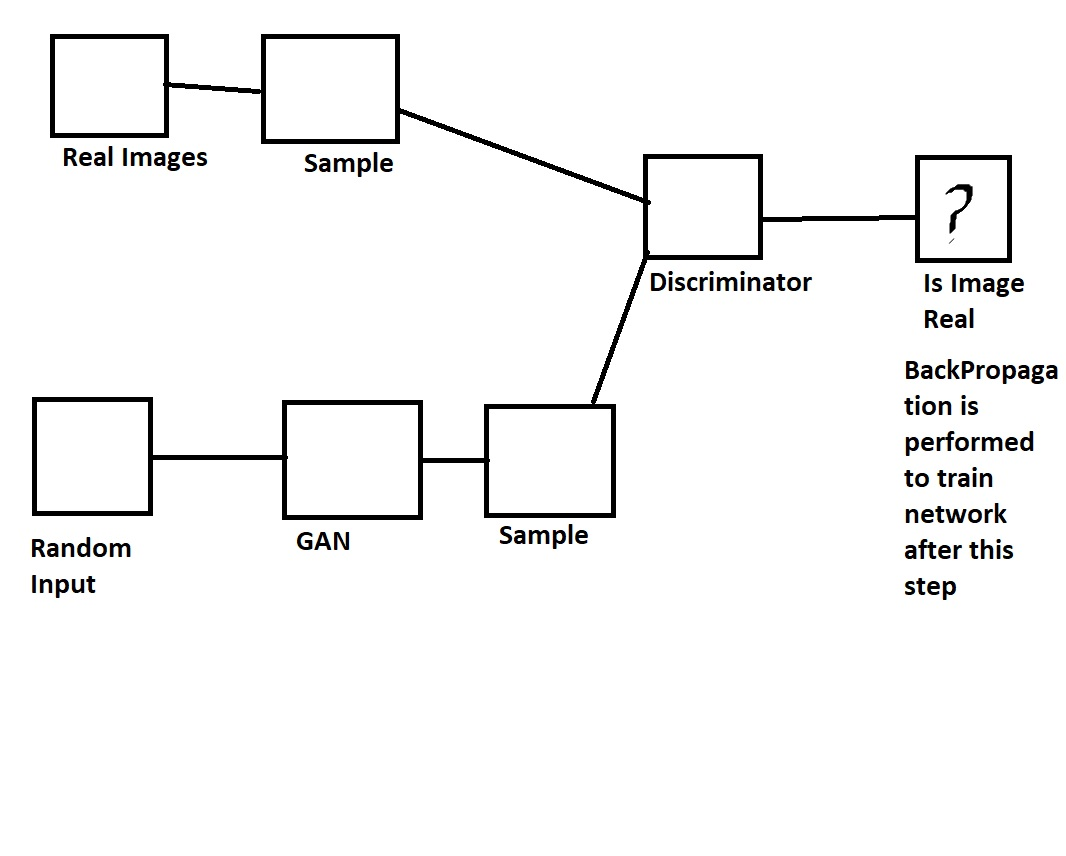
\includegraphics[width=1\textwidth,height=10cm]{Images/GAN Basic.jpg}\\
    \caption{Basic Example of Generative Adversarial Network}
    \label{fig:Example GAN Diagram}
\end{figure}
\vspace{0.5mm}
As we can see from the image above \ref{fig:Example GAN Diagram}, we start the process by taking a sample of real images from the training data, then passing it to the discriminator. We also take a sample from the GAN created images and pass that to the discriminator which will then determine if the images are real are fake.  After the discriminator guesses if the image generated is good enough to be considered real in terms of quality then backpropagation is performed to train the model so that it can differentiate better between samples that came from the training set and those which came from the generator $G$.
\section{Explanation of Artificial Neural Networks (ANNs)}
Artificial Neural Networks, or ANNs for short, comprise of a network of neurons or nodes(both terms can be used interchangeably) which are used for training a model to perform a certain task.  They are made up of an input layer, $N$ hidden layers, and finally an output layer.  Each layer has its own activation function and will adjust its weights and biases to determine the final output of the model.\cite{introToCnn} These networks are  heavily inspired by biological processes which occur in the brain.
\\
Artificial neural networks are a general-purpose model used to solve a number of common problems.
\vspace{0.5mm}
\begin{figure}[H]
    \centering
    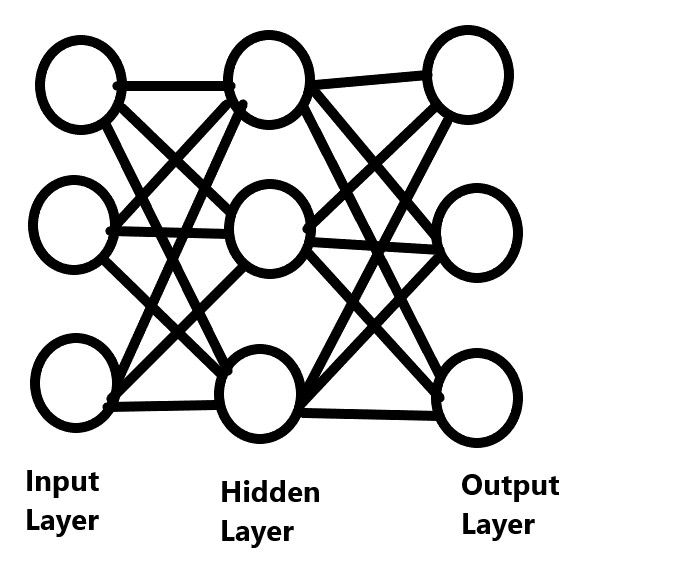
\includegraphics[width=0.5\textwidth]{Images/ANN Basic.jpg}\\
    \caption{Diagram of a Basic Artificial Neural Network with 1 input layer, 1 output layer, and 1 hidden layer}
    \label{fig:Example ANN Diagram}
\end{figure}
\vspace{0.5mm}

A basic example of an artificial neural network is shown in Figure \ref{fig:Example ANN Diagram}. As shown in the figure, the network has an input layer, a hidden layer, and an output layer.  Generally when creating these networks we determine the number of neurons in both the input and the output layers based on the number of classes we are trying to predict.  The above network could be used to predict if an image is of a cat, a dog, or a fish for example.  There can multiple hidden layers in an ANN and the number of neurons in each layer can be adjusted.  In reality, artificial neural networks will typically be far bigger than the example given above in terms of neurons and hidden layers but for illustrative purposes, the above diagram will suffice.  Each neuron will also have its own weight, bias, and an activation function which will determine whether a neuron fires or not. There are many common activation functions such as swish, ReLU (Rectified Linear Units), sigmoid, and tanh the use of which depends on a number of factors.
\section{What is A Convolutional Neural Network? (CNN)}
A convolutional neural network, or CNN for short, is a type of neural network which is primarily used for tasks involving image and pattern recognition\cite{introToCnn}. The structure is similar to an ANN in which we have an input layer, $N$ hidden layers, and finally an output layer.  As with the Artificial Neural Network each of these layers will have an activation function and its own weights and biases to determine the final output for a given input. The model will take an image as input, the image is made up of vectors (RGB) or a similar format and from that image the model will determine certain patterns. For example, the output might be a classification of whether or not COVID-19 is present. This application will be discussed in more detail later in the dissertation. 
\\
There are a few ways in which CNNs differ from ANNs, in that they are comprised of three types of layers which are the convolutional layers, pooling layers, and fully connected layers\cite{introToCnn}.  The convolutional layer is responsible for extracting features from an image and generating a $2D$ activation map, the pooling layer will reduce the parameters of a given input by means of downsampling, and finally the fully connected layers will then determine and classify the output for a given input.  The convolutional layer's parameters utilize learnable kernels (a kernel acts as a filter used to extract features from images), and this layer also produces a $2D$ activation map which will be used to determine if a neuron fires or not for a given input.  We can adjust hyper parameters in the convolutional layer to greatly reduce the complexity of the model through optimization, which can be achieved by adjusting the following hyper parameters: depth, stride and zero padding.
\\
Depth is related to the output volume produced by the convolutional layers in the model which can be manually set by adjusting the number of neurons in each layer.  Reducing the depth of the model can greatly decrease the training time but at the expense of performance.
\\
Stride is related to the spatial dimensionality of the input which will determine the receptive field (this is an area where each neuron in the network is connected to a small region of the input - this area of the network is called the receptive field\cite{introToCnn}), if the stride is set to a low integer we will produce extremely large activations, and if it is set too high the network won't produce enough activations.  The stride can also be interpreted as sliding a window across the image / video, where only a section of the image or video is input into the network at a time.
\\
Finally, zero-padding will pad the border of the images ingested by the model with 0s, reducing their dimensionality. Padding can prove to be useful in increasing the accuracy of the model as it can possibly eliminate areas of the image which are not useful for the model and can also improve training time times in some use cases\cite{zeroPaddingTrainingTime}.
\\
Through the adjustment of the hyperparameters mentioned above, and through the utilization of different activation functions, the accuracy of the convolutional neural network can be improved through a process of trial and error.
\section{Supervised Learning}
Supervised learning is a methodology of machine-learning involving the use of labeled data to train the model\cite{supervisedVsUnsupervised}. The data is typically labeled manually by a data scientist, which can be a long and laborious process depending on a number of factors (size of the data, number of classes, etc.), but offers many benefits when it comes to training models.  Supervised learning performs extremely well at tasks involving classification (classifying data into a given category), and regression (understanding the relationships between independent and dependent variables). 
\section{Unsupervised Learning}
Unsupervised learning is a methodology of machine-learning which involves using unlabelled data to train machine learning models\cite{supervisedVsUnsupervised}.  This type of machine learning requires no human intervention since the data is unlabelled and the model will detect relationships between data based on the raw data fed in to the model.  This type of machine learning is used for tasks such as: clustering (grouping data together based on shared characteristics or features), association (finding relationships between features), and dimensionality reduction (reducing the number of features in a given dataset without compromising the integrity of said data).  The key differences between supervised and unsupervised learning are: labeled versus unlabeled datasets, and finding relationships in data (unsupervised) or trying to predict and classify data (supervised).
\section{Tensorflow}
Tensorflow is an open-source library which allows developers to access a number of functions to make machine learning easier and allows developers to build models more quickly\cite{tensorflow}.  Tensorflow provides numerous modules and classes which form the foundation for building both the generative adversarial network and the convolutional neural network. There have been numerous case studies proving the efficacy of Tensorflow in solving many AI / ML problems and the library is used by research teams in organisations such as Google, Airbnb, ARM, Coca-Cola, Intel, and many more\cite{tensorflowCaseStudies}.  
\\
Given the reputation and widespread use of Tensorflow, and the vast amount of documentation around the framework, it seems  an ideal library for the implementation of GANs and CNNs for this study.
\section{Keras}
Keras is a deep-learning framework for Python developed by Francois Chollet which provides a number of helpful functions and methods for creating AI models\cite{keras}. Keras is built on top of Tensorflow and simplifies data loading, pre-processing and the overall building of the model.  Keras is commonly used by data-scientists and researchers due to the powerful methods it offers and the time it saves.  The additional classes and modules Keras provides on top of Tensorflow will help to reduce the time taken to build and develop of building both the convolutional neural network and the generative adversarial network.  
\\
Like Tensorflow, Keras has been used by a number of companies and is well recognised in the Artificial Intelligence community.  The framework has a range of uses and has proven beneficial when developing AI models in a number of areas and fields\cite{kerasExamples}.
\section{Background of Problem \& Aims of This Paper}
COVID-19 is a highly transmissible virus which has caused a worldwide pandemic and has claimed many lives. There have been 616,951,418 cases worldwide and 6,530,281 deaths as of the 4th of October 2022\cite{covid19StatsWorldwide}.  During the pandemic, Ireland alone was subject to a total of 1.6 million confirmed cases and nearly 8,000 deaths\cite{covid19StatsIreland}.  This has led many researchers to pursue the goal of automating the detection of COVID-19 to partially relieve the immense pressure put on medical staff throughout the pandemic. 
\vspace{0.5mm}
\begin{figure}[H]
    \centering
    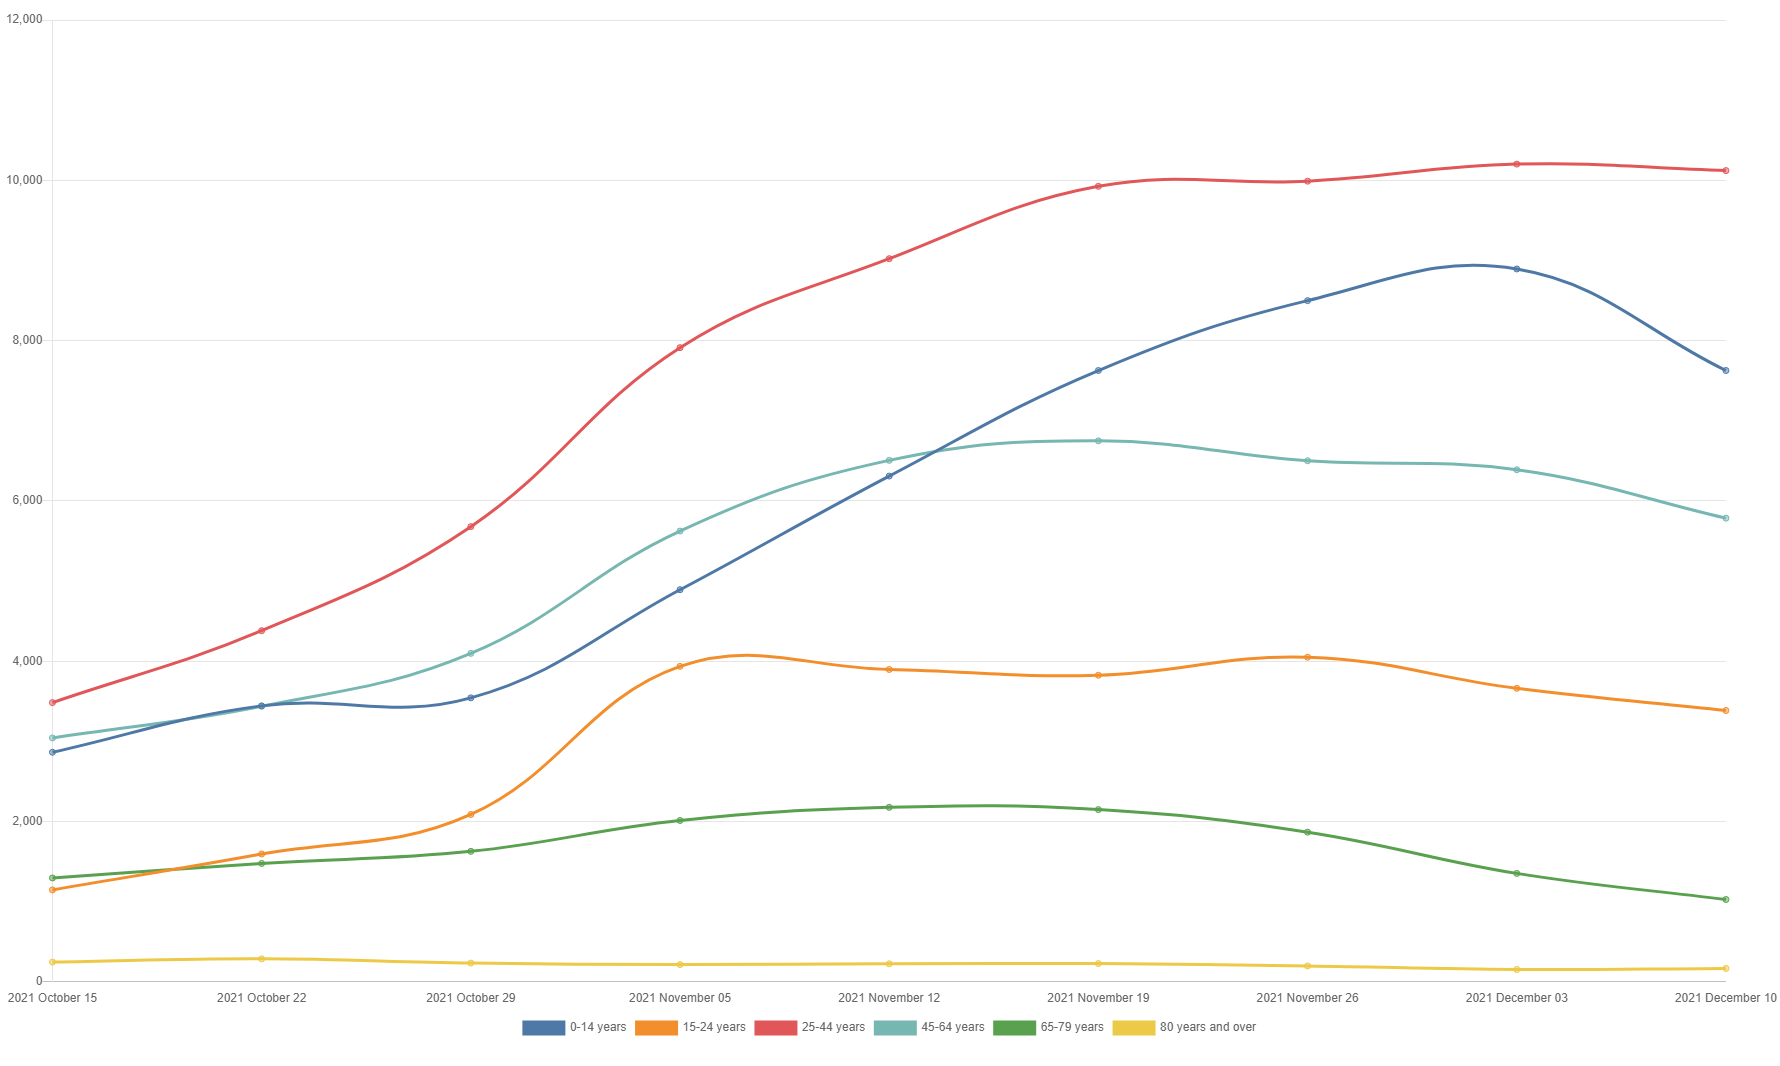
\includegraphics[width=1\textwidth,keepaspectratio]{Images/COVID19IrelandFigures.png}\\
    \caption{Graph of COVID-19 Statistics by age-range Ireland from October 2021 - December 2021 Courtesy of CSO\cite{csoCovid19Stats}}
    \label{fig:COVID-19 Ireland Statistics}
\end{figure}
\begin{figure}[H]
    \centering
    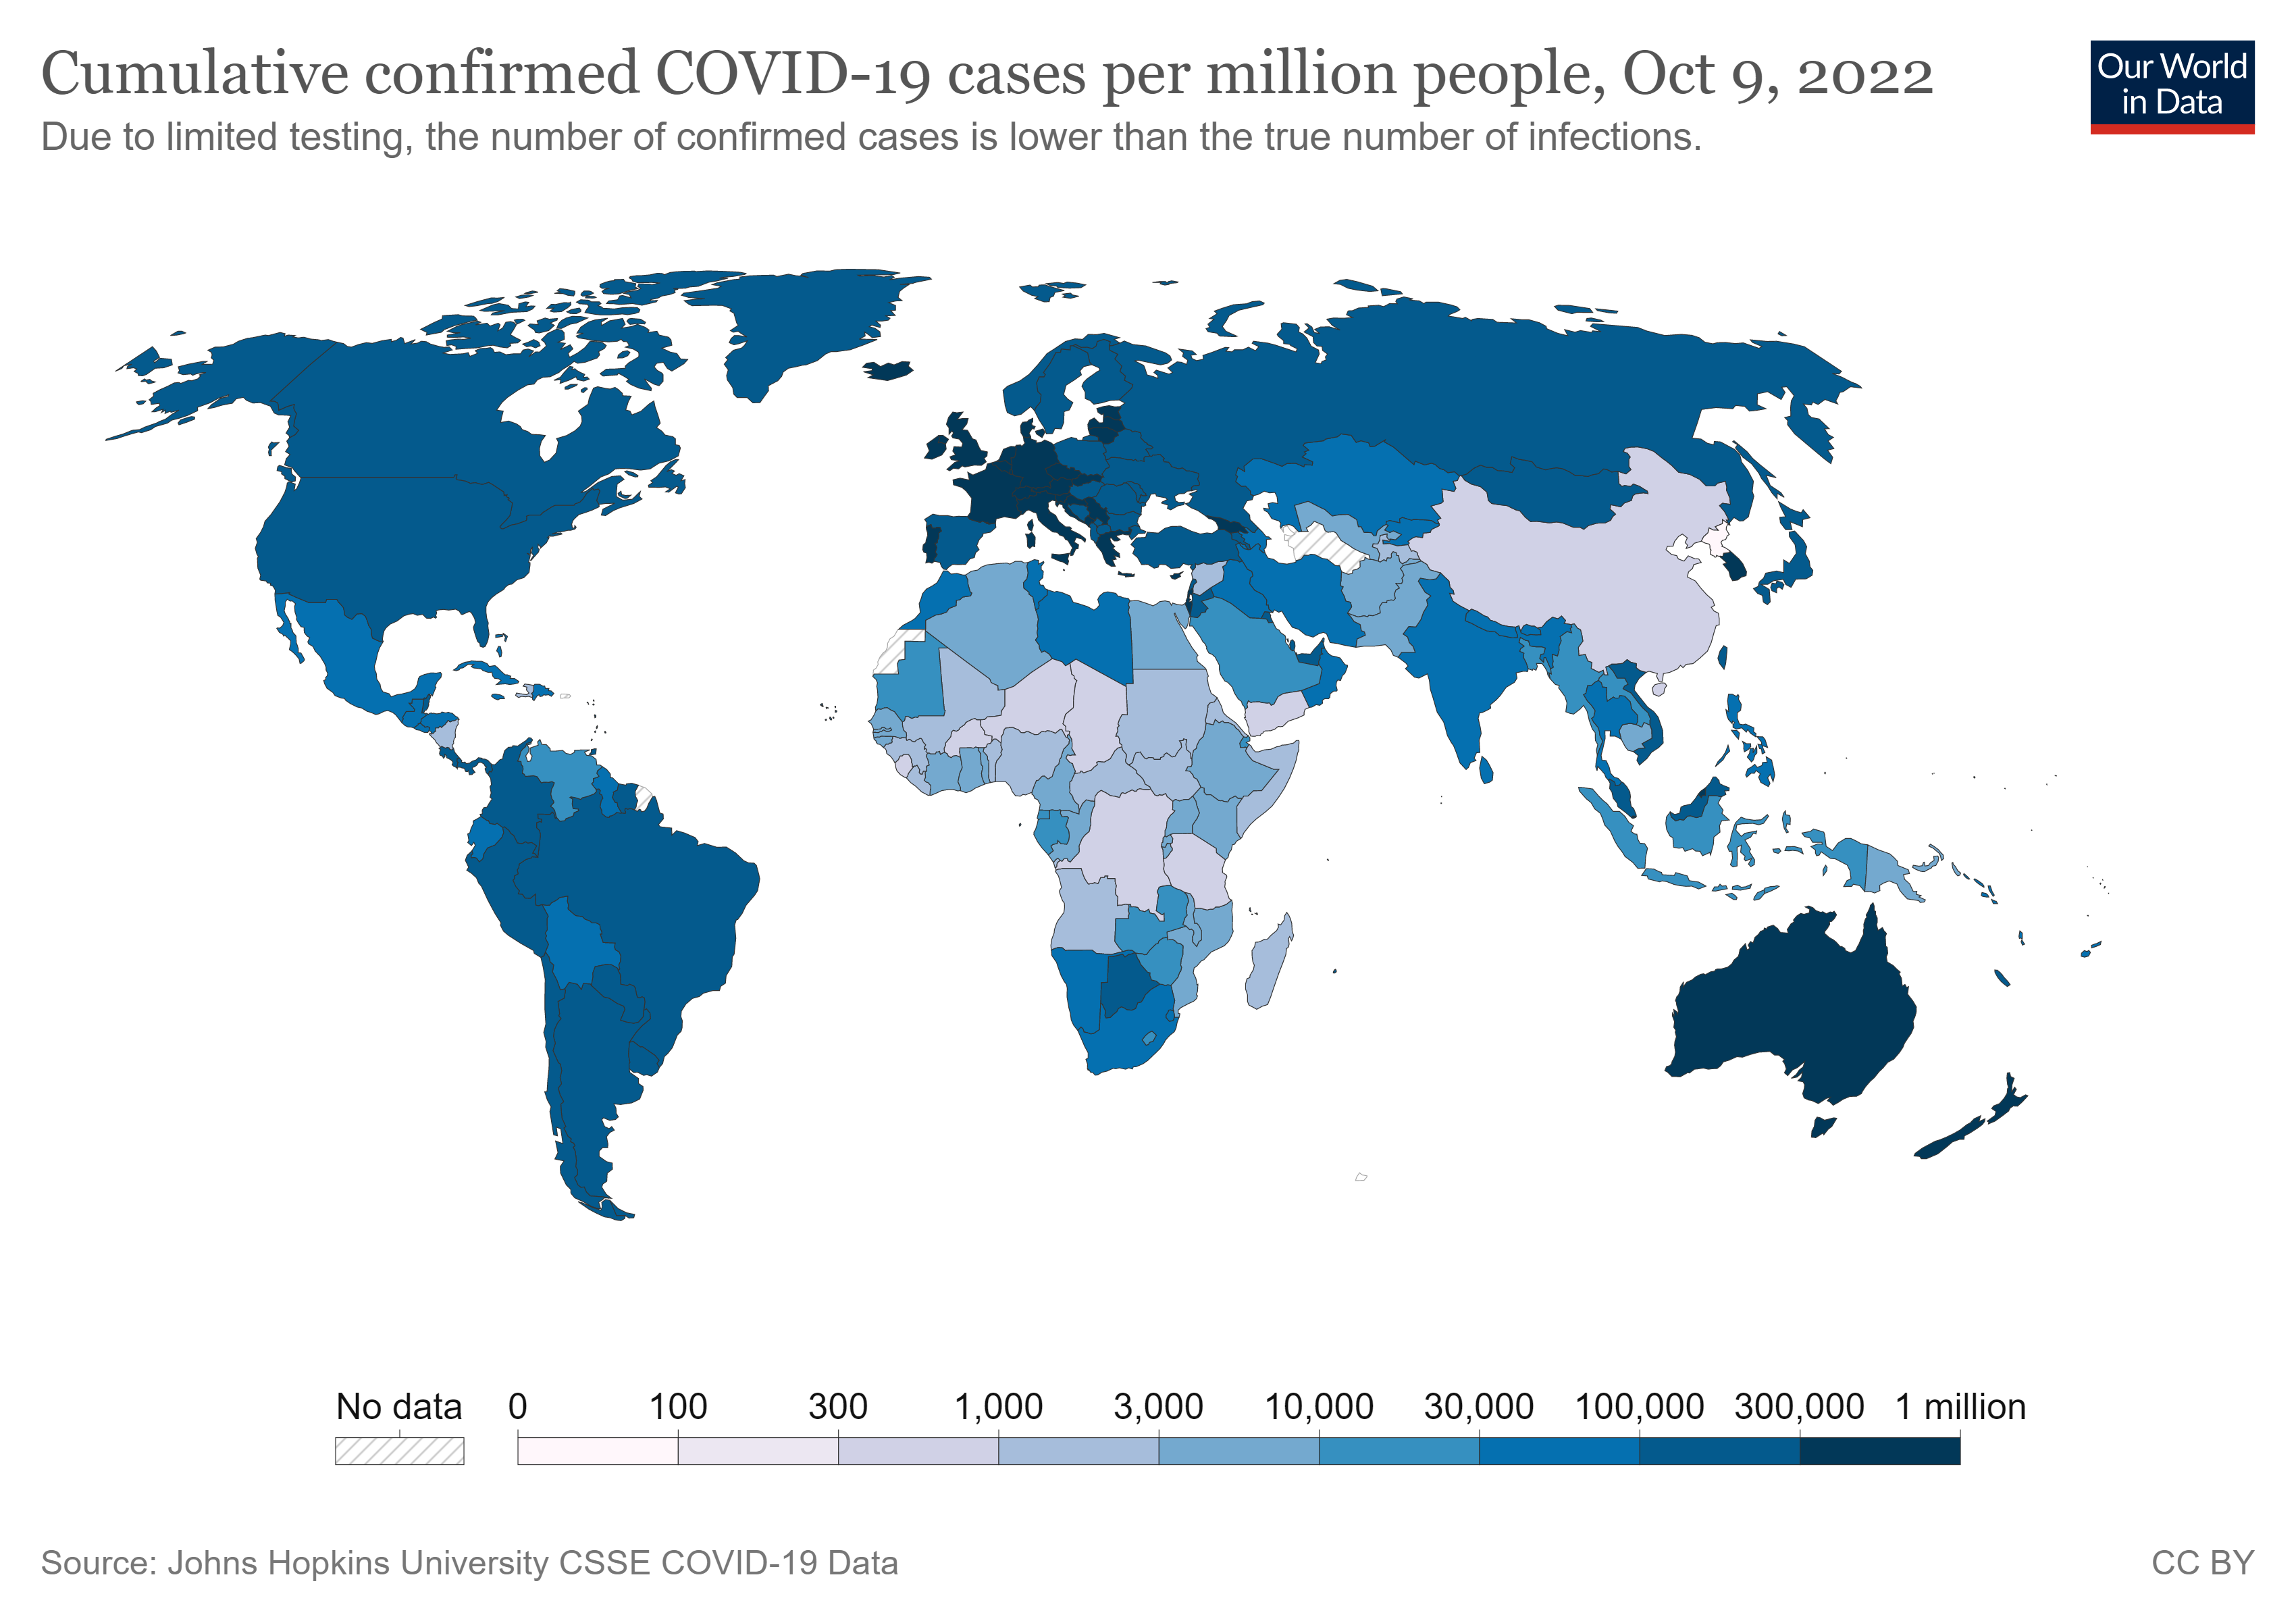
\includegraphics[width=1\textwidth,keepaspectratio]{Images/coronavirusWorldWide.png}\\
    \caption{Cumulative cases of the COVID-19 virus worldwide courtesy of Our World in Data\cite{cumulativeCovid19Cases}}
    \label{fig:COVID-19 Worldwide Statistics}
\end{figure}
\vspace{0.5mm}
The main objective of this research is to develop a robust model which can accurately analyze X-rays of patients and determine from said X-rays if the patient is afflicted with COVID-19.  This will be achieved by utilizing a number of different GAN architectures which will create realistic ''fake data'' which will then be used to train a number of models. From this training we plan to compare and contrast the results when generating data with different architectures to determine the best configuration for data generation to train the CNN model.  There has been some success in utilizing convolutional neural networks to automate the detection of the virus\cite{cnnCOVID19DetectionAhmed}\cite{cnnCOVID19DetectionLopez}.  Through the use of synthetic data generated by utilizing a variety of GAN architectures, it is our hope that such convolutional models will be improved upon and made more accurate.
\\
We plan on utilizing existing data sets which are listed in the next section when training the Generative Adversarial Models, through trial and error we plan on determining the best architecture of GANs to use for training the model for this use-case.
% Include stats and explain COVID 19 virus
\section{Datasets}
Before beginning the training of the model it is important to explore and understand each of the datasets.  There are a total of three datasets which will be used in the course of this research, we will explain more about these datasets below.
\subsection{COVID-19 Chest X-ray}
The COVID-19 Chest X-ray data set is a data set which is comprised of labeled X-ray Images taken from a number of patients. This dataset contains 357 X-ray images of COVID positive patients, and Chest X-rays of those afflicted with another disease (MERS, SARS, and ARDS).  This dataset also includes a metadata file listing the diagnosis of the patient along with a number of other features\cite{xrayDataset}. In total this dataset contains 11 classes, the images do not have a consistent resolution which may cause issues as resizing each image may lead to a loss in image quality.  The loss in quality will cause problems when evaluating the model's accuracy.
\\
\subsection{COVID-19 Radiography Database}
The COVID-19 Radiography Database is made up of 3,616 images of chest X-rays taken from COVID positive patients, 10,192 Images of lung X-rays taken from healthy patients, and 1,345 X-ray images of viral pneumonia positive patients. All images in this dataset are PNG (Portable Network Graphic) images and are at a resolution of height 299 pixels and width 299 pixels eliminating the need for preprocessing of the images, the dataset also includes metadata for each of the images in this dataset showing a number of features with the diagnosis of the patient as well. The data in this dataset was gathered by a team of researchers from Qatar University, Doha, Qatar, and the University of Dhaka, Bangladesh along with their collaborators from Pakistan and Malaysia\cite{radiography}.
\\
\subsection{COVID-19 Pneumonia Normal Chest X-ray PA Dataset}
The COVID-19 Pneumonia Normal Chest X-ray PA dataset is comprised of a train set containing 74 Normal X-ray Images taken from healthy Patients and  afflicted with Pneumonia and a test set containing a Normal set containing 20 chest X-rays taken from healthy patients and a Pneumonia set containing 20 images.  The images in this dataset are unlabelled and no metadata is offered, however, the images are segregated into separate files listing the diagnosis\cite{covidDataset}.
\\
\subsection{Extensive COVID-19 X-ray and CT Chest Images Dataset}
This dataset was added fairly late in the project due to data limitations in both the COVID-19 Chest X-ray and the COVID-19 Pneumonia Normal Chest X-ray PA Dataset.  This dataset is comprised of 17099 X-ray and CT images which were generated with various augmentation techniques.  Some of the images in this dataset come from the previously mentioned datasets namely the COVID-19 Pneumonia Normal Chest X-ray PA Dataset and the COVID-19 Chest X-ray.  Given the large number of images in this dataset it may prove useful when training GANs to reproduce images as some of the other datasets have proven to lack the data needed to reasonably train a GAN to reproduce the X-rays.
\\
The dataset is broken up into two folders containing X-rays and CT Scans respectively. Both folders contain images which are categorized into two further subfolders 
one containing COVID Positive X-ray and CT-Scans and the other containing COVID negative X-ray and CT scans\cite{extendedCOVIDds}.
\\
\subsection{Use of datasets in This Project}
we plan to use each of these datasets to train and test the model and use data augmentation to increase the train and test sets by utilizing Generalized Adversarial Networks.  When using these datasets in conjunction it is my hope that the GAN will have enough data to be effective when generating new sample images to train the final model.

\section{Structure of This Thesis}
This thesis is broken into 5 chapters in total, this section will include the headings of the chapters and a brief summary of each chapter below:

\subsection{Chapter 1 - Introduction} 
This chapter will offer the reader of this thesis a brief introduction to a number of core concepts which will be necessary to understand before diving deeper into this thesis.  It is important that the reader has a basic understanding of generative adversarial networks, convolutional neural networks, artificial neural networks, supervised \& unsupervised learning, and the overall question that this research proposes before discussing the implementation or discussing pertinent literature in this field. 
\\
In this section we will frame the research question, explain what a generative adversarial network is, its function, and how it works,  We will also explain artificial neural networks and convolutional neural networks, and we will discuss the basic methodologies relating to the implementation of this project.  We will also discuss the libraries used to implement the practical artifact, datasets used to train the model and give the reader of this thesis a clear understanding of the key aims of this research.
\subsection{Chapter 2 - Literature Review} 
In this section we will review pertinent literature related to the problem domain and discuss the ideas and concepts presented in these papers. We will also review the results from the research conducted in these papers and use them as a metric to gauge the performance of my own model.  The papers will also be compared and contrasted and we will discuss the findings and how useful these papers were when conducting my own research.  It is very important to understand the problem domain before beginning the implementation of this project to ensure that we are not "reinventing the wheel".  This section will also provide the reader of this thesis with the most up-to-date progress made within the problem domain.
\subsection{Chapter 3 - Implementation}
In this section we will discuss the architecture of the convolutional model, the various architectures of generative adversarial networks implemented, how the models were trained and the overall design of the code implemented, and the rationale behind certain design choices. we will also show the results from training the models and discuss how through trial and error we were able to improve the various models and will include code samples so that the models can be reviewed by the reader or re-implemented by them.
\subsection{Chapter 4 - Results}
In this section, we will review the results achieved from training the best models and suggest how they may possibly be improved.  we will be showing lots of graphs/tables in this section to gauge each model's test/dev set errors and we will also be comparing and contrasting the effects of the different GAN architectures implemented as well as discussing the results of the convolutional model.
\subsection{Chapter 5 - Further Research and Conclusions}
In this section, we will discuss further research that may need to be done by any researchers who would like to build upon this research.  we will also review where the models could be improved and what we'd do differently if we were to conduct this research again. we will also discuss common issues we faced during the implementation of this project and how we overcame them. This section will be a summary of all the research conducted, the code, and my experience overall throughout the writing of this thesis.  
\\
This will be the final section of the paper and will tie the entire thesis together.  

 

\include{Chapter 2 Literature Review}
\chapter{Design and Implementation}
\section{Introduction}
Initially, when starting the development of this model, we looked at various tools and options to implement the model in code.  We settled on using Jupyter Notebooks along with a number of libraries to help make the development of this model easier and faster.  The useful thing about Jupyter Notebooks is that Jupyter Notebooks can be opened in a browser and all the code can be run from a single page.  We will detail the development of our proposed model both in this thesis and include notes in the notebook itself to explain my rationale behind implementing the model in a certain way.  During the initial phase of implementation, I used both the Keras documentation \cite{keras} and Tensorflow documentation \cite{tensorflow} as references to ensure that the model's development was following standard practices and to ensure that the model was optimized to allow training in a timely manner. 
\\
Due to the limited support for AMD graphics cards (currently the GPU in our system has a 6700XT which does not have RoCM support\cite{amdLimitations}) in a variety of popular AI frameworks/libraries at the time of writing this thesis, we decided it was best to use Google Colab Pro when training both the CNNs and the GANs this may offer some limitations in terms of memory and computational power.  Google Colab Pro, however, does offer a lot of advantages when it comes to quickly setting up an environment in which to train these models, it is for this reason that we have chosen to use it for training the models.
\\
For the purpose of reproducible results, we included the following lines of code \texttt{np.random.seed(9)} and set the random seed of Keras to 10 so that other researchers can reproduce similar results (achieving the same results depends on a number of factors) and build upon this study.  All the datasets are loaded and split using a seed of 1337 also so that the train/test split is the exact same every time.  Each model also uses a train / validation / test split of 70\% for train, 10\% for validation and 20\% for test(bar the chest X-ray COVID 19 dataset).  The rationale for having double the amount of data for the test set when compared with the validation set was made so that the test set could have more variety and therefore a higher degree of accuracy when comparing / contrasting the models.
\section{CNN Model Design and Comparison}
In this section we will compare and contrast each CNN's architecture and design when evaluating on both the original datasets and augmented datasets.  The goal of this section is to determine which architecture works best when creating the automated diagnostic system and whether or not the augmented dataset is increasing the model's generalization ability and the model's accuracy. Initially when training the models we thought about using early-stopping to improve the accuracy and reduce the loss of these models, we decided against this due to the harm it may cause the model's generalization ability.  All the models listed below use the entire data available when they are being trained.
\subsection{Baseline Models}
When starting the implementation phase, we decided to use the following resource to develop baseline CNN models \cite{imageClassificationKeras}.  We plan on modifying this resource to achieve a relatively high training/validation accuracy when training on the original dataset.  We plan on using these models to get a metric with which we can compare models generated on the original dataset to the models which are generated on the synthetic dataset.  It is in this way we can accurately compare the effects of the synthetic dataset on the accuracy of the implemented models.
\\
After this initial comparison is done with the models trained on the original dataset versus the models trained on the synthetic dataset.  We then plan on focusing on which architectures would work best when developing the CNN and how the models trained on the synthetic dataset can be improved.
\\
To start we decided to use the following settings when developing a CNN to be used when training on the x-ray COVID-19 dataset.  This dataset is made up of images that are labeled either 1 or 0 with 1 being COVID-positive and 0 being COVID-negative.  We have included the architecture of the layers of the model in the table below \ref{tab: X-ray COVID-19 dataset CNN baseline model architecture}
\begin{table}[H]
    \centering
    \resizebox{\textwidth}{!}{
    \begin{tabular}{|c|c|c|c|c|c|c|}
    \hline
        Layer Number 
        & Layer Type
        & Layer Size 
        & Kernel Size
        & Strides
        & Padding
        & Activation\\
        \hline
        1 & Conv2D Layer & 16 & (3,3) & 2 & Same & Swish\\
        2 & SeparableConv2D Layer & 32 & (3,3) & None & Same & Swish \\
        3  & SeparableConv2D Layer & 64 & (3,3) & None & Same & Swish \\
        4  & MaxPooling2D & 2 & 2 & None & Same & None \\
        5 & Residual & 64 & (3,3) & 2 & Same & Swish \\
        6 & SeparableConv2D & 128 & (3,3) & None & Same & Swish \\
        7 & GlobalAveragePooling2D & 1 & None & None & None & Sigmoid \\
        \hline
    \end{tabular}
        }
    \caption{ X-ray COVID-19 dataset CNN baseline model architecture}
    \label{tab: X-ray COVID-19 dataset CNN baseline model architecture}
\end{table}
For the padding the keyword ''same'' means that the input is padded with 0s evenly, both up and down and left and right of the image. The input was also scaled to normalize the data using the following line of code ''1.0 / 255)(inputs)''  After each layer batch normalization was performed excluding the residual, max pooling, and global average pooling 2D layers.  The use of the activation function ``swish`` was chosen due to studies showing it's performance matched or outperformed ReLU for certain tasks\cite{swishAndRelu}. Swish differs slightly in comparison to ReLU in that there isn't a sharp rise as the weight approaches 0. 
 \begin{figure}[H]
    \centering
    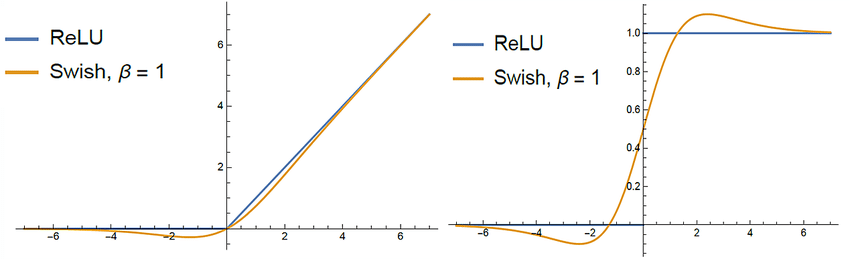
\includegraphics[width=1\textwidth,height=15cm,keepaspectratio]{Images/Swish ReLU activations.PNG}\\
    \caption{Figure of Swish and ReLU activation functions(Image courtesy of Madhura Ingalhalikar)\cite{swishReluDiagram}}
    \label{fig:Figure of Swish and ReLU activation functions}
\end{figure}
The model uses a dropout of 0, given the small size of the dataset we didn't want to drop neurons from the network. We also used the following settings when using model.compile() 
\begin{table}[H]
    \centering
    \resizebox{\textwidth}{!}{
    \begin{tabular}{|c|c|c|c|c|c|}
    \hline
         Optimizer
         & Loss Function 
         & Metric
         & Batch Size
         & Steps Per Epoch
         & Number of Epochs\\
         \hline
         Adam with a learning rate of $1\times10^{-3}$ & Binary CrossEntropy & Accuracy & 16 & 10 & 10\\
         \hline
    \end{tabular}
    }
    \caption{X-ray COVID-19 dataset CNN baseline model hyperparameters}
    \label{tab:X-ray COVID-19 dataset CNN baseline model hyperparameters}
\end{table}
The model was trained for a total of 37 epochs with 1 step per epoch (again due to the limitations in the size of the dataset) and achieved the following results.

\begin{table}[H]
    \centering
    \resizebox{\textwidth}{!}{
    \begin{tabular}{|c|c|c|c|c|c|}
    \hline
         Training Loss
         & Training Accuracy 
         & Validation Loss
         & Validation Accuracy
         & Test Set Loss
         & Test Set Accuracy\\
         \hline
         0.2651 & 0.9122 & 0.7918 & 0.5000 & 0.8173 & 0.4688\\
         \hline
    \end{tabular}
    }
    \caption{X-ray COVID-19 dataset CNN baseline model results}
    \label{tab:X-ray COVID-19 dataset CNN baseline model results}
\end{table}
 \begin{figure}[H]
    \centering
    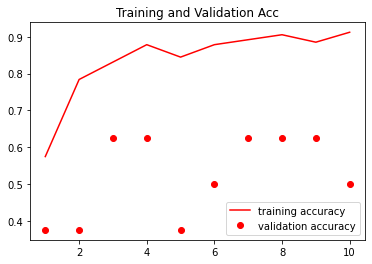
\includegraphics[width=1\textwidth,height=5cm,keepaspectratio]{Images/X-ray COVID-19 dataset CNN Train and Val Acc.png}\\
    \caption{Figure of Train and Validation Accuracy of X-ray COVID-19 dataset CNN Baseline Model  - The X-Axis shows the epoch number and the Y-axis shows the accuracy}
    \label{fig:X-ray COVID-19 dataset CNN Baseline Train and Validation Accuracy}
\end{figure}
 \begin{figure}[H]
    \centering
    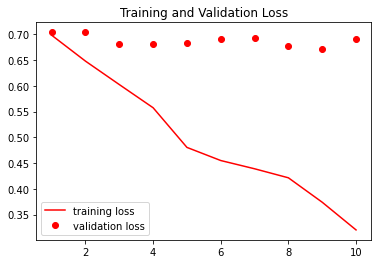
\includegraphics[width=1\textwidth,height=5cm,keepaspectratio]{Images/X-ray COVID-19 dataset CNN Train and Val Loss.png}\\
    \caption{Figure of Train and Validation Loss of X-ray COVID-19 dataset CNN Baseline Model  - The X-Axis shows the epoch number and the Y-axis shows the loss}
    \label{fig:X-ray COVID-19 dataset CNN Baseline Train and Validation Loss}
\end{figure}
As is shown from the results above \ref{tab:X-ray COVID-19 dataset CNN baseline model results} the model appears to be overfitting.  The model has a training accuracy which is 0.4122 higher than the validation accuracy.  The training loss is also much lower at 0.2651 when compared with the validation loss which is 0.7918.  The model overfitting the training set is expected given the small size of the dataset.  The model also performs very poorly on the test set and has a comparatively high loss and low accuracy when compared with the training set, which again is due to the limited data available.
\\
After finishing the CNN implementation for the X-ray COVID-19 dataset we then moved on to designing the model with the radiography dataset. This dataset is much larger than the original dataset, the radiography dataset contains a total of 30,306 image files broken into three classes.  In comparison, the X-ray COVID-19 dataset only contains 188 images belonging to two classes.  When designing this Convolutional network more thought had to be given to the split and which activation function to use for output, given that there are multiple classes.  When designing the CNN we decided to implement a much larger neural network given the amount of data available.  We tried using the initial network which was used for the X-ray COVID-19 dataset but the results were poor, increasing the size of the network led to better results.  Due to computational limitations we have decided to opt for ReLU instead of Swish as an activation function.
\begin{table}[H]
    \centering
    \resizebox{\textwidth}{!}{
    \begin{tabular}{|c|c|c|c|c|c|c|}
    \hline
        Layer Number 
        & Layer Type
        & Layer Size 
        & Kernel Size
        & Strides
        & Padding
        & Activation\\
        \hline
        1 & Conv2D Layer & 64 & (3,3) & 2 & Same & ReLU\\
        2 & SeparableConv2D Layer & 128 & (3,3) & 2 & Same & ReLU \\
        3  & SeparableConv2D Layer & 256 & (3,3) & 2 & Same & ReLU \\
        4 & SeparableConv2D Layer & 512 & (3,3) & 2 & Same & ReLU \\
        5  & MaxPooling2D & 3 & 2 & None & Same & None \\
        6 & Residual & 512 & (3,3) & 2 & Same & ReLU \\
        7 & SeparableConv2D & 1024 & (3,3) & None & Same & ReLU \\
        8 & GlobalAveragePooling2D & 3 & None & None & None & Softmax \\
        \hline
    \end{tabular}
    }
    \caption{Radiography CNN baseline model architecture}
    \label{tab:Radiography CNN baseline model architecture}
\end{table}


    \begin{table}[H]
    \centering
    \resizebox{\textwidth}{!}{
    \begin{tabular}{|c|c|c|c|c|c|}
    \hline
         Optimizer
         & Loss Function 
         & Metric
         & Batch Size
         & Steps Per Epoch
         & Number of Epochs\\
         \hline
         Adam with a learning rate of $1\times10^{-3}$ & sparse categorical crossentropy & Accuracy & 32 & 663 & 10\\
         \hline
    \end{tabular}
    }
    \caption{Radiography CNN baseline model hyperparameters}
    \label{tab:Radiography CNN baseline model hyperparameters}
\end{table}
In this model we achieved a higher accuracy when using ReLU as opposed to swift. The final results of the model are as follows:
\begin{table}[H]
    \centering
    \resizebox{\textwidth}{!}{
    \begin{tabular}{|c|c|c|c|c|c|}
    \hline
         Training Loss
         & Training Accuracy 
         & Validation Loss
         & Validation Accuracy
         & Test Set Loss
         & Test Set Accuracy\\
         \hline
         0.3446  & 0.8611 & 0.4120 & 0.8306 & 0.3800 & 0.8434\\
         \hline
    \end{tabular}
    }
    \caption{Radiography CNN baseline results}
    \label{tab:Radiography CNN baseline results}
\end{table}
 \begin{figure}[H]
    \centering
    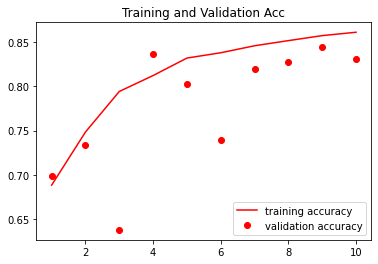
\includegraphics[width=1\textwidth,height=5cm,keepaspectratio]{Images/RadiographyCNNBaselineTrainAndValAcc.png}\\
    \caption{Train and Validation Accuracy of Radiography CNN Baseline Model - The X-Axis shows the epoch number and the Y-axis shows the accuracy}
    \label{fig:Radiography CNN Baseline Train and Validation Accuracy}
\end{figure}
 \begin{figure}[H]
    \centering
    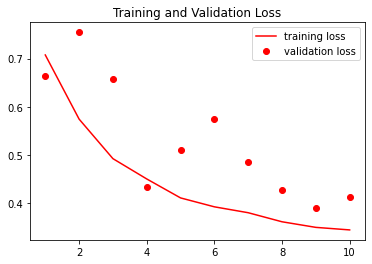
\includegraphics[width=1\textwidth,height=5cm,keepaspectratio]{Images/RadiographyCNNBaselineTrainAndValLoss.png}\\
    \caption{Figure of Train and Validation Loss of Radiography CNN Baseline Model - The X-Axis shows the epoch number and the Y-axis shows the loss}
    \label{fig:Second CNN Baseline Train and Validation Loss}
\end{figure}
As shown in the table \ref{tab:Radiography CNN baseline results} above we can see that the model has better results when compared with the first baseline model. One of the reasons for this is that we are dealing with a much larger dataset so the model has more images that it can learn features from, this yields a much higher accuracy when compared with the first baseline model which was trained on a much more limited dataset.
\\
The third baseline CNN model was trained using the COVID-19 chest X-ray dataset. This dataset didn't have a standardised resolution for images so the images had to be resized which could possibly lead to lack of data quality and consistency when resized.  For these models no test set was included as the some classes had very little data and it was impossible to include all classes when randomly sampling the data,  If data was manually included this would introduce bias so the test set was excluded from the model's evaluation.  When training the model there was a high degree of validation loss which is to be expected given the dataset size. The architecture of this model is as follows: 
\begin{table}[H]
    \centering
    \resizebox{\textwidth}{!}{
    \begin{tabular}{|c|c|c|c|c|c|c|}
    \hline
        Layer Number 
        & Layer Type
        & Layer Size 
        & Kernel Size
        & Strides
        & Padding
        & Activation\\
        \hline
        1 & Conv2D Layer & 32 & (3,3) & 2 & Same & Swish\\
        2 & SeparableConv2D Layer & 64 & (3,3) & 2 & Same & Swish \\
        3 & SeparableConv2D Layer & 128 & (3,3) & 2 & Same & Swish \\
        4 & SeparableConv2D Layer & 256 & (3,3) & 2 & Same & Swish \\
        5 & SeparableConv2D Layer & 512 & (3,3) & 2 & Same & Swish \\
        6  & MaxPooling2D & 3 & 2 & None & Same & None \\
        7 & Residual & 512 & (3,3) & 2 & Same & Swish \\
        8 & SeparableConv2D & 128 & (3,3) & None & Same & Swish \\
        9 & GlobalAveragePooling2D & 11 & None & None & None & Softmax \\
        \hline
    \end{tabular}
    }
    \caption{COVID-19 chest X-ray CNN baseline model architecture for COVID-19 Chest X-ray Dataset}
    \label{tab:COVID-19 chest X-ray CNN baseline model architecture}
\end{table}

    \begin{table}[H]
    \centering
    \resizebox{\textwidth}{!}{
    \begin{tabular}{|c|c|c|c|c|c|}
    \hline
         Optimizer
         & Loss Function 
         & Metric
         & Batch Size
         & Steps Per Epoch
         & Number of Epochs\\
         \hline
         Adam with a learning rate of $1\times10^{-3}$ & categorical crossentropy & Accuracy & 4 & 79 & 10\\
         \hline
    \end{tabular}
    }
    \caption{COVID-19 chest X-ray CNN baseline model hyperparameters for COVID-19 Chest X-ray Dataset}
    \label{tab:COVID-19 chest X-ray CNN baseline model hyperparameters}
\end{table}
Due to the small size of the dataset the batch size was set to a low number. The steps per epoch and number of epochs were also relatively low when compared with the other datasets due to the limited amount of data present.  The model's performance is shown in the table below:
\begin{table}[H]
    \centering
    \begin{tabular}{|c|c|c|c|}
    \hline
         Training Loss
         & Training Accuracy 
         & Validation Loss
         & Validation Accuracy\\
         \hline
         0.8372  & 0.7975 & 7.2848 & 0.6571\\
         \hline
    \end{tabular}
    \caption{COVID-19 chest X-ray CNN baseline model results for COVID-19 Chest X-ray Dataset}
    \label{tab:COVID-19 chest X-ray CNN baseline model results}
\end{table}
 \begin{figure}[H]
    \centering
    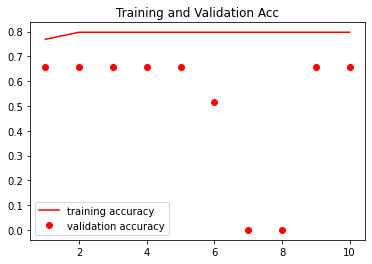
\includegraphics[width=1\textwidth,height=5cm,keepaspectratio]{Images/ChestXrayCNNBaselineTrainAndValAcc.png}\\
    \caption{Figure of Train and Validation Accuracy of COVID-19 chest X-ray CNN Baseline Model - The X-Axis shows the epoch number and the Y-axis shows the accuracy}
    \label{fig:COVID-19 chest X-ray CNN Baseline Train and Validation Accuracy}
\end{figure}
 \begin{figure}[H]
    \centering
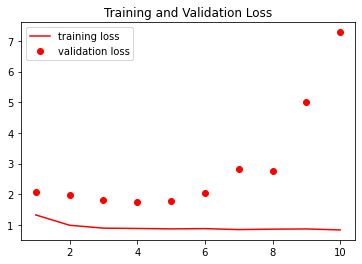
\includegraphics[width=1\textwidth,height=5cm,keepaspectratio]{Images/ChestXrayCNNBaselineTrainAndValLoss.png}\\
    \caption{Figure of Train and Validation Loss of COVID-19 chest X-ray CNN Baseline Model - The X-Axis shows the epoch number and the Y-axis shows the loss}
    \label{fig:COVID-19 chest X-ray CNN Baseline Train and Validation Loss}
\end{figure}
As shown in table \ref{tab:COVID-19 chest X-ray CNN baseline model results} the model has a high degree of loss and the accuracy isn't very good on either the training or the validation set.  This is to be expected as the dataset is quite small and contains a large number of classes.  The model suffers from insufficient data and has performed poorly due to data imbalance as well as lack of standardised image resolutions.
\\
The fourth and fifth baseline models were trained using the Extensive COVID Dataset.  This dataset is comprised of two different categories of images, one category of images being X-ray images and the other being CT scans.  Two different CNNs were trained, one was trained using the X-ray images and the other using the CT images.  The first baseline model for the Extensive COVID Dataset was trained on the CT images and the second baseline model was trained using the X-ray images.
\\
When creating the baseline model we trialled a number of different architectures the best performing of these architectures is shown in table \ref{tab:Extensive COVID-19 CT Dataset CNN Baseline Model Architecture}
\begin{table}[H]
    \centering
    \resizebox{\textwidth}{!}{
    \begin{tabular}{|c|c|c|c|c|c|c|}
    \hline
        Layer Number 
        & Layer Type
        & Layer Size 
        & Kernel Size
        & Strides
        & Padding
        & Activation\\
        \hline
        1 & Conv2D Layer & 32 & (3,3) & 2 & Same & ReLU\\
        2 & SeparableConv2D Layer & 64 & (3,3) & 2 & Same & ReLU \\
        3  & SeparableConv2D & 128 & None & None & Same & ReLU \\
        4 & SeparableConv2D & 256 & (3,3) & None & Same & ReLU \\
        5 & SeparableConv2D & 512 & (3,3) & None & Same & ReLU \\
        6 & residual & 512 & (3,3) & 2 & Same & ReLU \\
        7 & SeparableConv2D & 1024 & (3,3) & None & None & ReLU \\
        8 & activation layer & 1 & None & None & None & Sigmoid \\

        \hline
    \end{tabular}
    }
    \caption{Extensive COVID-19 CT Dataset CNN baseline model architecture}
    \label{tab:Extensive COVID-19 CT Dataset CNN Baseline Model Architecture}
\end{table}
\begin{table}[H]
    \centering
    \resizebox{\textwidth}{!}{
    \begin{tabular}{|c|c|c|c|c|c|}
    \hline
         Optimizer
         & Loss Function 
         & Metric
         & Batch Size
         & Steps Per Epoch
         & Number of Epochs\\
         \hline
         RMSprop with a learning rate of $1\times10^{-3}$ and a momentum of $1\times10^{-3}$ & binary crossentropy & Accuracy & 32 & 177 & 10\\
         \hline
    \end{tabular}
    }
    \caption{Extensive CT CNN baseline model hyperparameters}
    \label{tab:Extensive CT CNN baseline model hyperparameters}
\end{table}
\begin{table}[H]
    \centering
    \resizebox{\textwidth}{!}{
    \begin{tabular}{|c|c|c|c|c|c|}
    \hline
         Training Loss
         & Training Accuracy 
         & Validation Loss
         & Validation Accuracy
         & Test Set Loss
         & Test Set Accuracy\\
         \hline
         0.2286 & 0.9023 & 0.3837 & 0.8150 & 0.3574 & 0.8319\\
         \hline
    \end{tabular}
    }
    \caption{Extensive CT CNN baseline model results}
    \label{tab:Extensive CT CNN baseline model results}
\end{table}
The training / validation accuracy and loss for this model are visible in the images included below
 \begin{figure}[H]
    \centering
    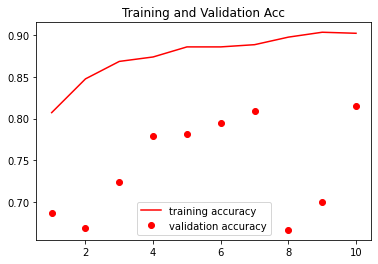
\includegraphics[width=1\textwidth,height=5cm,keepaspectratio]{Images/ExtensiveCNNBaselineModelExtensiveCovidAccCT.png}\\
    \caption{Figure of Train and Validation accuracy of Extensive COVID CNN Baseline Model CT  - The X-Axis shows the epoch number and the Y-axis shows the accuracy}
    \label{fig:Extensive COVID CT CNN Baseline Model CNN Baseline Train and Validation Accuracy}
\end{figure}
 \begin{figure}[H]
    \centering
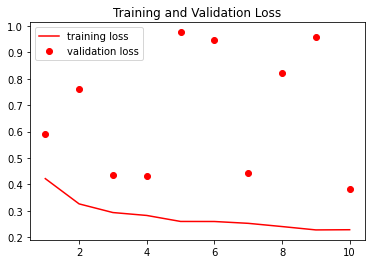
\includegraphics[width=1\textwidth,height=5cm,keepaspectratio]{Images/ExtensiveCNNBaselineModelExtensiveCovidLossCT.png}\\
    \caption{Figure of Train and Validation Loss of Extensive COVID CNN Baseline Model CT  - The X-Axis shows the epoch number and the Y-axis shows the loss}
    \label{fig:Extensive COVID CT CNN Baseline Model CNN Baseline Train and Validation Loss}
\end{figure}
When creating the baseline model we trialled a number of different architectures but found the following architecture detailed in table \ref{tab:Extensive COVID-19 X-Ray CNN Baseline Model Architecture}
\begin{table}[H]
    \centering
    \resizebox{\textwidth}{!}{
    \begin{tabular}{|c|c|c|c|c|c|c|}
    \hline
        Layer Number 
        & Layer Type
        & Layer Size 
        & Kernel Size
        & Strides
        & Padding
        & Activation\\
        \hline
        1 & Conv2D Layer & 32 & (3,3) & 2 & Same & ReLU\\
        2 & SeparableConv2D Layer & 64 & (3,3) & 2 & Same & ReLU \\
        3  & SeparableConv2D & 128 & None & None & Same & ReLU \\
        4 & SeparableConv2D & 256 & (3,3) & None & Same & ReLU \\
        5 & SeparableConv2D & 512 & (3,3) & None & Same & ReLU \\
        6 & residual & 512 & (3,3) & 2 & Same & ReLU \\
        7 & SeparableConv2D & 1024 & (3,3) & None & None & ReLU \\
        8 & activation layer & 1 & None & None & None & Sigmoid \\

        \hline
    \end{tabular}
    }
    \caption{Extensive COVID-19 X-Ray CNN Baseline Model Architecture}
    \label{tab:Extensive COVID-19 X-Ray CNN Baseline Model Architecture}
\end{table}
\begin{table}[H]
    \centering
    \resizebox{\textwidth}{!}{
    \begin{tabular}{|c|c|c|c|c|c|}
    \hline
         Optimizer
         & Loss Function 
         & Metric
         & Batch Size
         & Steps Per Epoch
         & Number of Epochs\\
         \hline
         RMSprop with a learning rate of $10^{-3}$ and a momentum of $10^{-3}$ & binary crossentropy & Accuracy & 32 & 209 & 10\\
         \hline
    \end{tabular}
    }
    \caption{Extensive COVID-19 X-Ray CNN baseline model hyperparameters}
    \label{tab:Extensive COVID-19 X-Ray CNN baseline model hyperparameters}
\end{table}
\begin{table}[H]
    \centering
    \resizebox{\textwidth}{!}{
    \begin{tabular}{|c|c|c|c|c|c|}
    \hline
         Training Loss
         & Training Accuracy 
         & Validation Loss
         & Validation Accuracy
         & Test Set Loss
         & Test Set Accuracy\\
         \hline
         0.1948 & 0.9278 & 0.3482 & 0.8587 & 0.3203 & 0.8698\\
         \hline
    \end{tabular}
    }
    \caption{Extensive COVID-19 X-Ray CNN baseline model results}
    \label{tab:Extensive COVID-19 X-Ray CNN baseline model results}
\end{table}
The training / validation accuracy and loss for this model are visible in the images included below
 \begin{figure}[H]
    \centering
    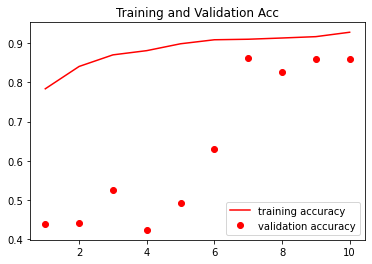
\includegraphics[width=1\textwidth,height=5cm,keepaspectratio]{Images/ExtensiveCOVID19XRayCNNBaselineModelAcc.png}\\
    \caption{Figure of Extensive COVID-19 X-ray CNN Baseline Model Train and Validation Accuracy - The X-Axis shows the epoch number and the Y-axis shows the accuracy}
    \label{fig:Extensive COVID-19 X-ray CNN Baseline ModelTrain and Validation Accuracy}
\end{figure}
 \begin{figure}[H]
    \centering
    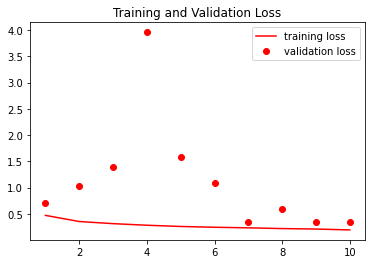
\includegraphics[width=1\textwidth,height=5cm,keepaspectratio]{Images/ExtensiveCOVID19XRayCNNBaselineModelLoss.png}\\
    \caption{Figure of Extensive COVID-19 X-ray CNN Baseline Model Train and Validation Loss  - The X-Axis shows the epoch number and the Y-axis shows the loss}
    \label{fig:Extensive COVID-19 X-ray CNN Baseline ModelTrain and Validation Loss}
\end{figure}
\section{Transfer Learning CNN Baseline Models}
Next we will compare the transfer learning baseline models. Keras offers a large number of pretrained models\cite{pretrainedModelsKeras}.  For the sake of time we have chosen the following three pretrained models to compare and contrast their effectiveness when automating COVID-19 diagnosis, Xception, ResNet50V2, and EfficientNetV2S were chosen as the architectures.  When choosing the pretrained models we had to carefully consider both their performance and size for use in this project.  Some models had parameters in excess of 100 million parameters which would not be usable in Colab Pro due to computational resource limitations.  Thus the models chosen had a reasonable number of parameters to avoid crashes when training the CNNs, the model with the highest number of parameters was ResNet50V2 which has 25.6M trainable parameters and the other two models have approximately 20 - 25 million parameters.  
\\
The weights used with all the transfer models come from models trained using the ImageNet dataset\cite{imageNet}.  The ImageNet dataset is comprised of 14,197,122 images and contains 1,000 classes.
\subsection{Radiography Dataset}
\subsubsection{Xception}
This model contains 21,386,795 parameters including a layer of 256 ReLU units and an additional layer of 3 softmax units which were appended to the model. The model ran for a total of 10 epochs with 663 steps per epoch.  The model also used sparse categorical cross entropy for the loss function and for the optimizer used Adam with a learning rate of $1\times10^{-3}$. The model achieved a final result of 0.9543 training accuracy with  0.1162  loss and had a validation accuracy of 0.8964 with a validation loss of 0.3867.  The model also has a test set accuracy of 0.9001 alongside a test set loss of 0.3833.  This is a relatively small but significant improvement in comparison to the original baseline models.  Figure \ref{fig:Transfer Learning Xception CNN Baseline Train and Validation Accuracy Radiography} shows the training and validation accuracy and figure \ref{fig:Transfer Learning Xception CNN Baseline Train and Validation Loss Radiography} shows the training and validation loss. 
 \begin{figure}[H]
    \centering
    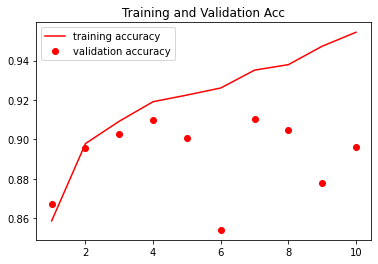
\includegraphics[width=1\textwidth,height=5cm,keepaspectratio]{Images/XceptionBaselineTrainingValidationAccRadiography.png}\\
    \caption{Transfer Learning Xception CNN Baseline Train and Validation Accuracy  - The X-Axis shows the epoch number and the Y-axis shows the accuracy}
    \label{fig:Transfer Learning Xception CNN Baseline Train and Validation Accuracy Radiography}
\end{figure}
 \begin{figure}[H]
    \centering    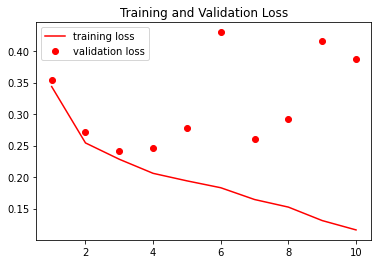
\includegraphics[width=1\textwidth,height=5cm,keepaspectratio]{Images/XceptionBaselineTrainingValidationLossRadiography.png}\\
    \caption{Transfer Learning Xception CNN Baseline Train and Validation Loss  - The X-Axis shows the epoch number and the Y-axis shows the loss}
    \label{fig:Transfer Learning Xception CNN Baseline Train and Validation Loss Radiography}
\end{figure}
\subsubsection{ResNet50V2}
This model had a total of 24,090,115 parameters including a layer of 256 ReLU units and an additional layer of 3 softmax units which were appended to the model.  This model had the same number of epochs and steps per epoch as exception(10 epochs with 663 steps) and also used the same optimizer with the same learning rate(Adam with $1\times10^{-3}$ as the learning rate).  The model performed slightly worse than Xception and finished with a training accuracy of 0.9172 and a training loss of 0.2024 and had a validation accuracy of 0.8695 with a validation loss of 0.3944.  The model also has a test set accuracy of 0.8809 and a test set loss of 0.3942.  Figure \ref{fig:Transfer Learning ResNet50V2 CNN Baseline Train and Validation Accuracy Radiography} shows the training and validation accuracy and figure \ref{fig:Transfer Learning ResNet50V2 CNN Baseline Train and Validation Loss Radiography} shows the training and validation loss. 
 \begin{figure}[H]
    \centering
    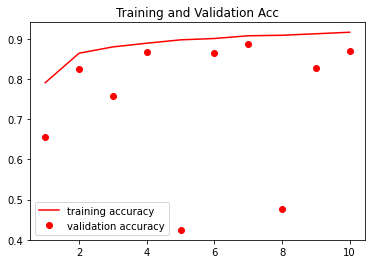
\includegraphics[width=1\textwidth,height=5cm,keepaspectratio]{Images/ResNet50V2BaselineTrainingValidationAccRadiography.png}\\
    \caption{Transfer Learning ResNet50V2 CNN Baseline Train and Validation Accuracy - The X-Axis shows the epoch number and the Y-axis shows the accuracy}
    \label{fig:Transfer Learning ResNet50V2 CNN Baseline Train and Validation Accuracy Radiography}
\end{figure}
 \begin{figure}[H]
    \centering
    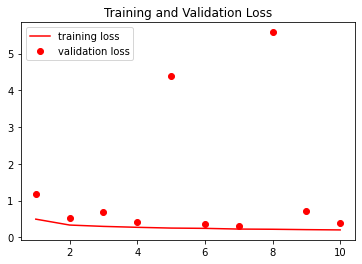
\includegraphics[width=1\textwidth,height=5cm,keepaspectratio]{Images/ResNet50V2BaselineTrainingValidationLossRadiography.png}\\
    \caption{Transfer Learning ResNet50V2 CNN Baseline Train and Validation Loss  - The X-Axis shows the epoch number and the Y-axis shows the loss}
    \label{fig:Transfer Learning ResNet50V2 CNN Baseline Train and Validation Loss Radiography}
\end{figure}
As shown in the figures above Xception outperforms this model when it comes to both the training accuracy and validation accuracy as well as the loss.
\subsubsection{EfficientNetV2S}
EfficientNetVS2 is a model with a total of 20,660,067 parameters including a layer of 256 ReLU units and an additional layer of 3 softmax units which were appended to the model.  Like the previous models this model was trained for a total of 10 epochs with 663 steps within each epoch.  It uses Adam as an optimizer with a learning rate of $1\times10^{-3}$.  The model performed worse than Xception but better than ResNet50V2 on the training,test, and validation sets. The model had a similar performance as Xception but managed to have a slightly lower train, test and validation accuracy and slightly lower losses for both the test and validation sets but a higher loss for the training set.  The model has a training accuracy of 0.9383 and a training loss of 0.1519 and a validation accuracy of 0.8844 and a validation loss of 0.3362.  The model also has a test loss of 0.3217 and a test accuracy of 0.8811. Figure \ref{fig:Transfer Learning EfficientNetV2S CNN Baseline Train and Validation Accuracy Radiography} shows the training and validation accuracy and figure \ref{fig:Transfer Learning EfficientNetV2S CNN Baseline Train and Validation Loss Radiography} shows the training and validation loss. 
 \begin{figure}[H]
    \centering
    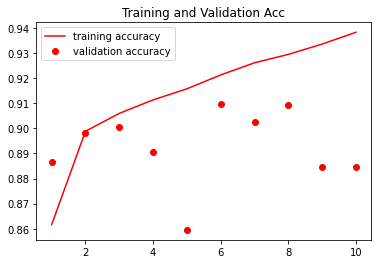
\includegraphics[width=1\textwidth,height=5cm,keepaspectratio]{Images/EfficientNetV2SBaselineTrainingValidationAccRadiography.png}\\
    \caption{Transfer Learning EfficientNetV2S CNN Baseline Train and Validation Accuracy  - The X-Axis shows the epoch number and the Y-axis shows the accuracy}
    \label{fig:Transfer Learning EfficientNetV2S CNN Baseline Train and Validation Accuracy Radiography}
\end{figure}
 \begin{figure}[H]
    \centering
    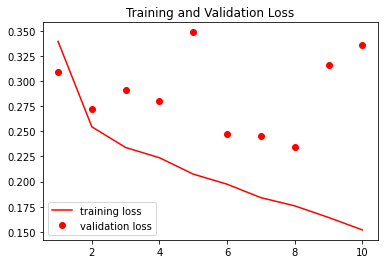
\includegraphics[width=1\textwidth,height=5cm,keepaspectratio]{Images/EfficientNetV2SBaselineTrainingValidationLossRadiography.png}\\
    \caption{Transfer Learning EfficientNetV2S CNN Baseline Train and Validation Loss  - The X-Axis shows the epoch number and the Y-axis shows the loss}
    \label{fig:Transfer Learning EfficientNetV2S CNN Baseline Train and Validation Loss Radiography}
\end{figure}
\subsection{X-Ray COVID-19 Dataset}
\subsubsection{Xception}
This model has a total of 22,960,681 parameters including a layer of 1024 ReLU units and a layer of 1 Sigmoid unit which were appended to the model. The model uses binary crossentropy as a loss function and uses Adam as an optimizer with a learning rate of $1\times10^{-3}$. 
The model ran for a total of 10 epochs with 10 steps per epoch.  The model achieved a training accuracy of 0.9662 with a training loss of 0.0951 and a validation accuracy of 0.5000 with a validation loss of 5.4697.  The model also had a test set loss of 7.5530 and a test set accuracy of 0.3750.  As with the baseline model this model is overfitting the training set which is to be expected given the small size of the dataset.  Figure \ref{fig:Xception CNN Baseline Train and Validation Accuracy X-Ray COVID19} shows the training and validation accuracy and figure \ref{fig:Xception CNN Baseline Train and Validation Loss X-Ray COVID19} shows the training and validation loss. 
 \begin{figure}[H]
    \centering
    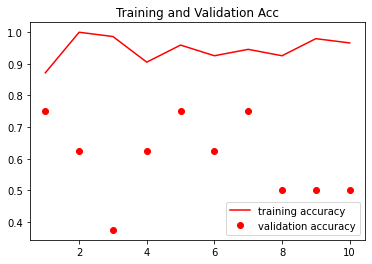
\includegraphics[width=1\textwidth,height=5cm,keepaspectratio]{Images/XceptionBaselineTrainingValidationAccuracyXRayCOVID19.png}\\
    \caption{Transfer Learning Xception CNN Baseline Train and Validation Accuracy X-Ray COVID19 - The X-Axis shows the epoch number and the Y-axis shows the accuracy}
    \label{fig:Xception CNN Baseline Train and Validation Accuracy X-Ray COVID19}
\end{figure}
 \begin{figure}[H]
    \centering
    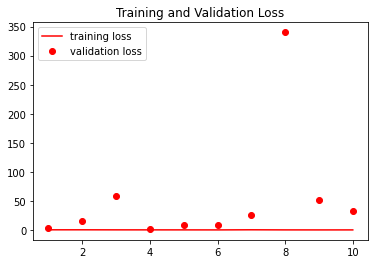
\includegraphics[width=1\textwidth,height=5cm,keepaspectratio]{Images/XceptionBaselineTrainingValidationLossXRayCOVID19.png}\\
    \caption{Transfer Learning Xception CNN Baseline Train and Validation Loss X-Ray COVID19 - The X-Axis shows the epoch number and the Y-axis shows the loss}
    \label{fig:Xception CNN Baseline Train and Validation Loss X-Ray COVID19}
\end{figure}
\subsubsection{ResNet50V2}
This model has a total of 25,664,001 parameters with an additional layer of 1024 ReLU units and another layer of 1 sigmoid unit which was appended to the model.  The model uses binary crossentropy as a loss function and Adam with a learning rate of $1\times10^{-3}$ as an optimizer.  The model ran for a total of 10 epochs with 10 steps per epoch and achieved a training accuracy of 0.9257 and a training loss of 0.2622 along with a validation accuracy of 0.3750 and a validation loss of 29.2193.  The model also has a high test loss of 23.9440 and an accuracy of 0.4688.  As with both the baseline and Xception models this model has overfit the training set. Figure \ref{fig:ResNet50V2 CNN Baseline Train and Validation Accuracy X-Ray COVID19} shows the training and validation accuracy and figure \ref{fig:ResNet50V2 CNN Baseline Train and Validation Loss X-Ray COVID19} shows the training and validation loss.
 \begin{figure}[H]
    \centering
    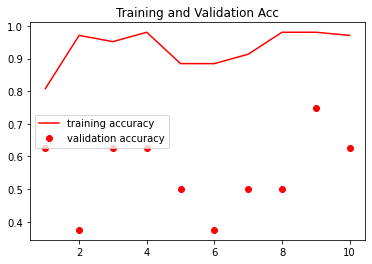
\includegraphics[width=1\textwidth,height=5cm,keepaspectratio]{Images/ResNet50V2BaselineTrainingValidationAccuracyXRayCOVID19.png}\\
    \caption{Transfer Learning ResNet50V2 CNN Baseline Train and Validation Accuracy X-Ray COVID19 - The X-Axis shows the epoch number and the Y-axis shows the accuracy}
    \label{fig:ResNet50V2 CNN Baseline Train and Validation Accuracy X-Ray COVID19}
\end{figure}
 \begin{figure}[H]
    \centering
    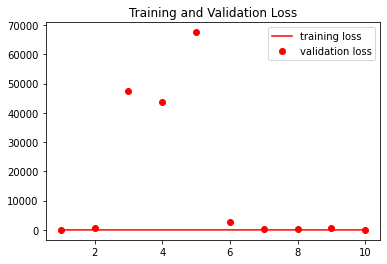
\includegraphics[width=1\textwidth,height=5cm,keepaspectratio]{Images/ResNet50V2BaselineTrainingValidationLossXRayCOVID19.png}\\
    \caption{Transfer Learning ResNet50V2 CNN Baseline Train and Validation Loss X-Ray COVID19 - The X-Axis shows the epoch number and the Y-axis shows the loss}
    \label{fig:ResNet50V2 CNN Baseline Train and Validation Loss X-Ray COVID19}
\end{figure}
\subsubsection{EfficientNetV2S}
This model has a total of 21,644,129 parameters with an additional layer of 1024 ReLU units and another layer of 1 sigmoid unit.  The model uses binary crossentropy as a loss funciton and Adam as an optimizer with a learning rate of $1\times10^{-3}$.  The model runs for a total of 10 epochs with 7 step per epoch. The model achieved a training accuracy of 1.000 with a training loss of 0.0063 and a validation accuracy of 1.0000 and a validation loss of 0.0011.  The model also achieved a test set loss of 0.2317 and a test set accuracy of 0.9375. Figure \ref{fig:EfficientNetV2S CNN Baseline Train and Validation Accuracy X-Ray COVID19} shows the training and validation accuracy and figure \ref{fig:EfficientNetV2S CNN Baseline Train and Validation Loss X-Ray COVID19} shows the training and validation loss. This model outperformed the baseline, Xception and ResNet50V2 models in terms of both loss and accuracy.
 \begin{figure}[H]
    \centering
    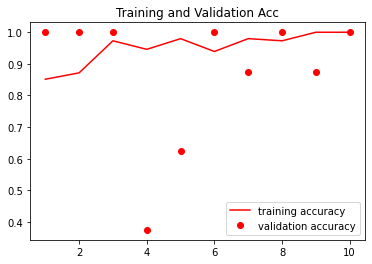
\includegraphics[width=1\textwidth,height=5cm,keepaspectratio]{Images/EfficientNetV2SBaselineTrainingValidationAccuracyXRayCOVID19.png}\\
    \caption{Transfer Learning EfficientNetV2S CNN Baseline Train and Validation Accuracy X-Ray COVID19 - The X-Axis shows the epoch number and the Y-axis shows the accuracy}
    \label{fig:EfficientNetV2S CNN Baseline Train and Validation Accuracy X-Ray COVID19}
\end{figure}
 \begin{figure}[H]
    \centering
    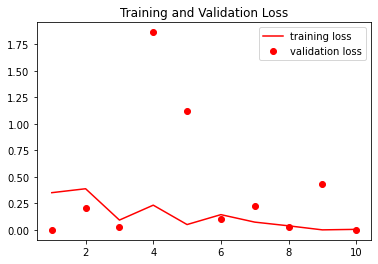
\includegraphics[width=1\textwidth,height=5cm,keepaspectratio]{Images/EfficientNetV2SBaselineTrainingValidationLossXRayCOVID19.png}\\
    \caption{Transfer Learning EfficientNetV2S CNN Baseline Train and Validation Loss X-Ray COVID19 - The X-Axis shows the epoch number and the Y-axis shows the loss}
    \label{fig:EfficientNetV2S CNN Baseline Train and Validation Loss X-Ray COVID19}
\end{figure}
\subsection{Evaluation of TL models for The x-ray covid 19 dataset}
The X-ray covid 19 dataset has a lack of data as it only comprises of 188 images.  It is not surprising to see that the models are greatly overfitting the training set.  Due to it's limited size this dataset may not be suitable for training GANs or the output of said GANs may lack diversity.
\subsection{COVID-19 Chest X-Ray Dataset}
\subsubsection{Xception}
This model has a total of 22,970,931 parameters including an additional layer of 1024 ReLU units and another layer of 11 softmax units which were appended to the model.  The model uses categorical crossentropy as a loss function along with Adam with a learning rate of $1 \times 10^{-3}$ as an optimizer.  The model runs for a total of 10 epochs with 79 step per epoch and achieved a training accuracy of 0.7975 and a training loss of 0.6109 along with a validation accuracy of 0.6571 and a validation loss of 1.6387. Figure \ref{fig:Xception CNN Baseline Train and Validation Accuracy Chest X-Ray} shows the training and validation accuracy and figure \ref{fig:Xception CNN Baseline Train and Validation Loss Chest X-Ray} shows the training and validation loss.
 \begin{figure}[H]
    \centering
    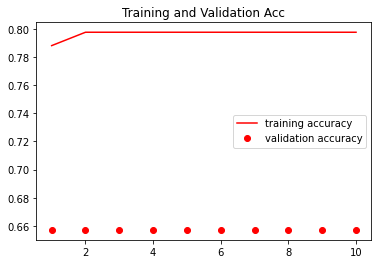
\includegraphics[width=1\textwidth,height=5cm,keepaspectratio]{Images/XceptionBaselineTrainingValidationAccuracyChestX-Ray.png}\\
    \caption{Transfer Learning Xception CNN Baseline Train and Validation Accuracy Chest X-Ray - The X-Axis shows the epoch number and the Y-axis shows the accuracy}
    \label{fig:Xception CNN Baseline Train and Validation Accuracy Chest X-Ray}
\end{figure}
 \begin{figure}[H]
    \centering
    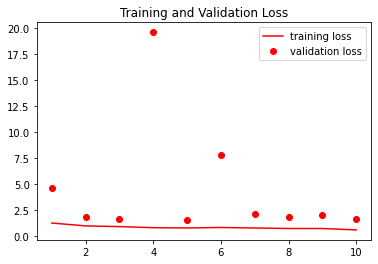
\includegraphics[width=1\textwidth,height=5cm,keepaspectratio]{Images/XceptionBaselineTrainingValidationLossChestX-Ray.png}\\
    \caption{Transfer Learning Xception CNN Baseline Train and Validation Loss X-Ray Chest X-Ray - The X-Axis shows the epoch number and the Y-axis shows the loss}
    \label{fig:Xception CNN Baseline Train and Validation Loss Chest X-Ray}
\end{figure}
\subsubsection{ResNet50V2}
This model has a total of 25,674,251 parameters including an additional layer of 1024 ReLU units and another layer of 11 softmax units which were appended to the model.  The model uses categorical crossentropy as a loss function along with Adam with a learning rate of $1 \times 10^{-3}$ as an optimizer.  The model runs for a total of 10 epochs with 79 step per epoch and achieved a training accuracy of 0.7975 and a training loss of 0.9676 along with a validation accuracy of 0.6571 and a validation loss of 1.5587. Figure \ref{fig:ResNet50V2 CNN Baseline Train and Validation Accuracy Chest X-Ray} shows the training and validation accuracy and figure \ref{fig:ResNet50V2 CNN Baseline Train and Validation Loss Chest X-Ray} shows the training and validation loss.
 \begin{figure}[H]
    \centering
    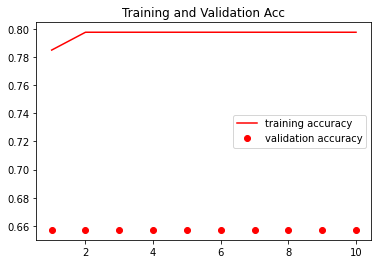
\includegraphics[width=1\textwidth,height=5cm,keepaspectratio]{Images/ResNet50V2BaselineTrainingValidationAccuracyChestX-Ray.png}\\
    \caption{Transfer Learning ResNet50V2 CNN Baseline Train and Validation Accuracy Chest X-Ray - The X-Axis shows the epoch number and the Y-axis shows the accuracy}
    \label{fig:ResNet50V2 CNN Baseline Train and Validation Accuracy Chest X-Ray}
\end{figure}
 \begin{figure}[H]
    \centering
    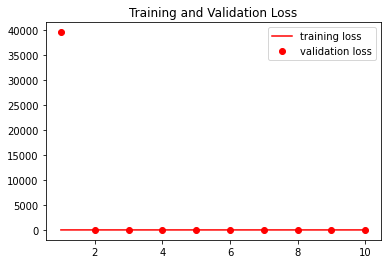
\includegraphics[width=1\textwidth,height=5cm,keepaspectratio]{Images/ResNet50V2BaselineTrainingValidationLossChestX-Ray.png}\\
    \caption{Transfer Learning ResNet50V2 CNN Baseline Train and Validation Loss X-Ray Chest X-Ray - The X-Axis shows the epoch number and the Y-axis shows the loss}
    \label{fig:ResNet50V2 CNN Baseline Train and Validation Loss Chest X-Ray}
\end{figure}
\subsubsection{EfficientNetV2S}
This model has a total of 21,654,379 parameters including an additional layer of 1024 ReLU units and another layer of 11 softmax units which were appended to the model.  The model uses categorical crossentropy as a loss function along with Adam with a learning rate of $1\times 10^{-2}$ as an optimizer.  The model runs for a total of 10 epochs with 79 step per epoch and achieved a training accuracy of 0.7975 and a training loss of 1.0280 along with a validation accuracy of 0.6571 and a validation loss of 1.7049. Figure \ref{fig:EfficientNetV2S CNN Baseline Train and Validation Accuracy Chest X-Ray} shows the training and validation accuracy and figure \ref{fig:EfficientNetV2S CNN Baseline Train and Validation Loss Chest X-Ray} shows the training and validation loss.
 \begin{figure}[H]
    \centering
    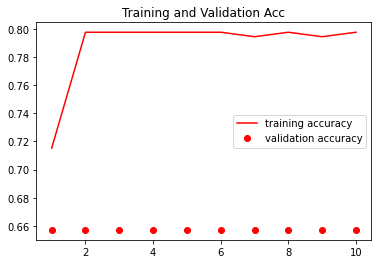
\includegraphics[width=1\textwidth,height=5cm,keepaspectratio]{Images/EfficientNetV2SBaselineTrainingValidationAccuracyChestX-Ray.png}\\
    \caption{Transfer Learning EfficientNetV2S CNN Baseline Train and Validation Accuracy Chest X-Ray - The X-Axis shows the epoch number and the Y-axis shows the accuracy}
    \label{fig:EfficientNetV2S CNN Baseline Train and Validation Accuracy Chest X-Ray}
\end{figure}
 \begin{figure}[H]
    \centering
    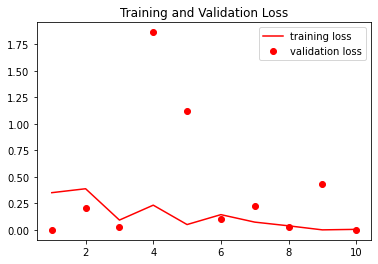
\includegraphics[width=1\textwidth,height=5cm,keepaspectratio]{Images/EfficientNetV2SBaselineTrainingValidationLossXRayCOVID19.png}\\
    \caption{Transfer Learning EfficientNetV2S CNN Baseline Train and Validation Loss Chest X-Ray - The X-Axis shows the epoch number and the Y-axis shows the loss}
    \label{fig:EfficientNetV2S CNN Baseline Train and Validation Loss Chest X-Ray}
\end{figure}
\subsection{Extensive COVID-19 Dataset CT}
\subsubsection{Xception}
This model is comprised of 21,386,281 parameters in total including an additional layer of 256 neurons using ReLU activation and an output layer of 1 neuron using a sigmoid activation function.  The model was trained for a total of 10 epochs with a total of 177 steps per epoch and uses RMSprop as an optimizer with a learning rate of $1\times10^{-3}$ and a momentum of $1\times10^{-3}$.  The model achieved a training accuracy of 0.9904 and a training loss of 0.0238 along with a validation accuracy of 0.9534 and a validation loss of 0.2250.  The model also had a test set loss of 0.1771 and a test accuracy of 0.9537. Figure \ref{fig:Xception CNN Baseline Train and Validation Accuracy Extensive COVID 19 Dataset CT} and figure \ref{fig:Xception CNN Baseline Train and Validation Loss Extensive COVID 19 Dataset CT} shows the training and validation loss.
 \begin{figure}[H]
    \centering
    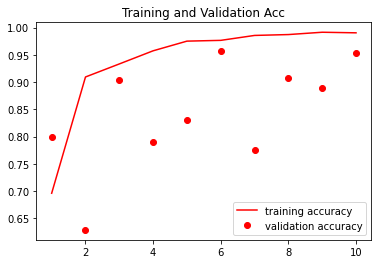
\includegraphics[width=1\textwidth,height=5cm,keepaspectratio]{Images/XceptionBaselineTrainingValidationAccuracyExtensiveCT.png}\\
    \caption{Transfer Learning Xception CNN Baseline Train and Validation Accuracy Extensive COVID 19 Dataset CT - The X-Axis shows the epoch number and the Y-axis shows the accuracy}
    \label{fig:Xception CNN Baseline Train and Validation Accuracy Extensive COVID 19 Dataset CT}
\end{figure}
 \begin{figure}[H]
    \centering
    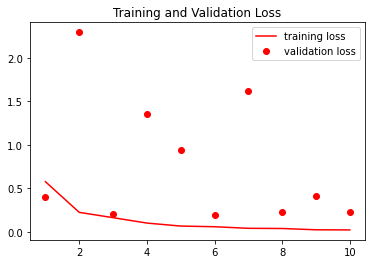
\includegraphics[width=1\textwidth,height=5cm,keepaspectratio]{Images/XceptionBaselineTrainingValidationLossExtensiveCT.png}\\
    \caption{Transfer Learning Xception CNN Baseline Train and Validation Loss Extensive COVID 19 Dataset CT - The X-Axis shows the epoch number and the Y-axis shows the loss}
    \label{fig:Xception CNN Baseline Train and Validation Loss Extensive COVID 19 Dataset CT}
\end{figure}
\subsubsection{ResNet50V2}
This model is comprised of 24,089,601 parameters in total including an additional layer of 256 neurons using ReLU activation and an output layer of 1 neuron using a sigmoid activation function.  The model was trained for a total of 10 epochs with 177 steps per epoch and uses RMSprop as an optimizer with a learning rate of $1\times10^{-3}$ and a momentum of $1\times10^{-3}$.  The model achieved a training accuracy of 0.9604 and a training loss of 0.1140 along with a validation accuracy of 0.9350 and a validation loss of 0.2078.  The model also has a test set accuracy of 0.9262 and a test set loss of 0.1993. Figure \ref{fig:ResNet50V2 CNN Baseline Train and Validation Accuracy Extensive COVID 19 Dataset CT} shows the training and validation accuracy and figure \ref{fig:ResNet50V2 CNN Baseline Train and Validation Accuracy Extensive COVID 19 Dataset CT} shows the training and validation loss.
 \begin{figure}[H]
    \centering
    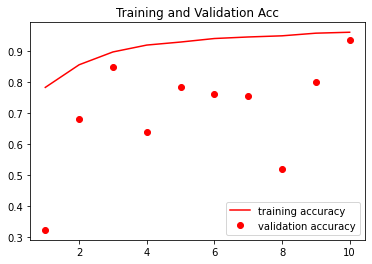
\includegraphics[width=1\textwidth,height=5cm,keepaspectratio]{Images/ResNet50V2BaselineTrainingValidationAccuracyExtensiveCT.png}\\
    \caption{Transfer Learning ResNet50V2 CNN Baseline Train and Validation Accuracy Extensive COVID 19 Dataset CT - The X-Axis shows the epoch number and the Y-axis shows the accuracy}
    \label{fig:ResNet50V2 CNN Baseline Train and Validation Accuracy Extensive COVID 19 Dataset CT}
\end{figure}
 \begin{figure}[H]
    \centering   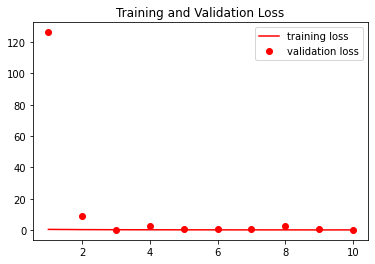
\includegraphics[width=1\textwidth,height=5cm,keepaspectratio]{Images/ResNet50V2BaselineTrainingValidationLossExtensiveCT.png}\\
    \caption{Transfer Learning ResNet50V2 CNN Baseline Train and Validation Loss Extensive COVID 19 Dataset CT - The X-Axis shows the epoch number and the Y-axis shows the loss}
    \label{fig:ResNet50V2 CNN Baseline Train and Validation Loss Extensive COVID 19 Dataset CT}
\end{figure}
\subsubsection{EfficientNetV2S}
This model is comprised of 20,659,553 parameters in total including an additional layer of 256 neurons using ReLU activation and an output layer of 1 neuron using a sigmoid activation function.  The model was trained for a total of 10 epochs with 177 steps per epoch and uses RMSprop as an optimizer with a learning rate of $1\times10^{-3}$ and a momentum of $1\times10^{-5}$.  The model achieved a training accuracy of 0.9901 and a training loss of 0.0291 along with a validation accuracy of 0.9375 and a validation loss of 0.2638.  The model also has a test set accuracy of 0.9438 and a test set loss of 0.2352. Figure \ref{fig:EfficientNetV2S CNN Baseline Train and Validation Accuracy Extensive COVID 19 Dataset CT} shows the training and validation accuracy and figure \ref{fig:EfficientNetV2S CNN Baseline Train and Validation Accuracy Extensive COVID 19 Dataset CT} shows the training and validation loss.
 \begin{figure}[H]
    \centering    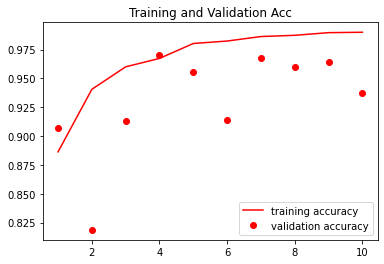
\includegraphics[width=1\textwidth,height=5cm,keepaspectratio]{Images/EfficientNetV2SBaselineTrainingValidationAccuracyExtensiveCT.png}\\
    \caption{Transfer Learning EfficientNetV2S CNN Baseline Train and Validation Accuracy Extensive COVID 19 Dataset CT - The X-Axis shows the epoch number and the Y-axis shows the accuracy}
    \label{fig:EfficientNetV2S CNN Baseline Train and Validation Accuracy Extensive COVID 19 Dataset CT}
\end{figure}
 \begin{figure}[H]
    \centering
    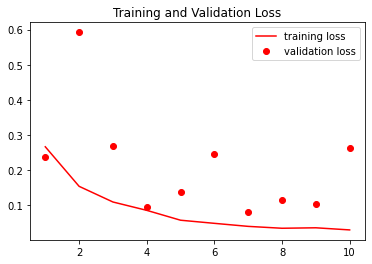
\includegraphics[width=1\textwidth,height=5cm,keepaspectratio]{Images/EfficientNetV2SBaselineTrainingValidationLossExtensiveCT.png}\\
    \caption{Transfer Learning EfficientNetV2S CNN Baseline Train and Validation Loss Extensive COVID 19 Dataset CT - The X-Axis shows the epoch number and the Y-axis shows the loss}
    \label{fig:EfficientNetV2S CNN Baseline Train and Validation Loss Extensive COVID 19 Dataset CT}
\end{figure}

\subsection{Extensive COVID-19 Dataset X-ray}
\subsubsection{Xception}
This model is comprised of 21,386,281 parameters in total including an additional layer of 256 neurons using ReLU activation and an output layer of 1 neuron using a sigmoid activation function.  The model was trained for a total of 10 epochs with a total of 177 steps per epoch and uses RMSprop as an optimizer with a learning rate of $1\times10^{-3}$ and a momentum of $1\times10^{-3}$.  The model achieved a training accuracy of 0.9876 and a training loss of 0.0277 along with a validation accuracy of 0.9416 and a validation loss of 0.2814.  The model also had a test set loss of 0.1947 and a test set accuracy of 0.9578. Figure \ref{fig:Xception CNN Baseline Train and Validation Accuracy Extensive COVID 19 Dataset X-ray} shows the training and validation accuracy and figure \ref{fig:Xception CNN Baseline Train and Validation Accuracy Extensive COVID 19 Dataset X-ray} shows the training and validation loss.
 \begin{figure}[H]
    \centering
    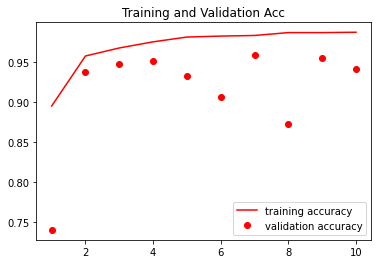
\includegraphics[width=1\textwidth,height=5cm,keepaspectratio]{Images/XceptionBaselineTrainingValidationAccuracyExtensiveXray.png}\\
    \caption{Transfer Learning Xception CNN Baseline Train and Validation Accuracy Extensive COVID 19 Dataset X-ray - The X-Axis shows the epoch number and the Y-axis shows the accuracy}
    \label{fig:Xception CNN Baseline Train and Validation Accuracy Extensive COVID 19 Dataset X-ray}
\end{figure}
 \begin{figure}[H]
    \centering
    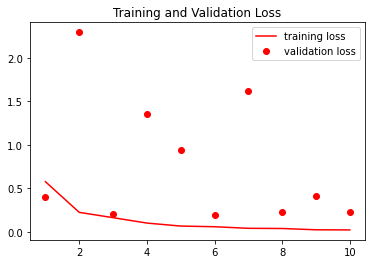
\includegraphics[width=1\textwidth,height=5cm,keepaspectratio]{Images/XceptionBaselineTrainingValidationLossExtensiveCT.png}\\
    \caption{Transfer Learning Xception CNN Baseline Train and Validation Loss Extensive COVID 19 Dataset X-ray - The X-Axis shows the epoch number and the Y-axis shows the loss}
    \label{fig:Xception CNN Baseline Train and Validation Loss Extensive COVID 19 Dataset X-ray}
\end{figure}
\subsubsection{ResNet50V2}
This model is comprised of 24,089,601 parameters in total including an additional layer of 256 neurons using ReLU activation and an output layer of 1 neuron using a sigmoid activation function.  The model was trained for a total of 10 epochs with 209 steps per epoch and uses RMSprop as an optimizer with a learning rate of $1\times10^{-3}$ and a momentum of $1\times10^{-3}$.  The model achieved a training accuracy of 0.9649 and a training loss of 0.0907 along with a validation accuracy of 0.9139 and a validation loss of 0.2842.  The model also has a test set accuracy of 0.9224 and a test set loss of 0.2379. Figure \ref{fig:ResNet50V2 CNN Baseline Train and Validation Accuracy Extensive COVID 19 Dataset X-ray} shows the training and validation accuracy and figure \ref{fig:ResNet50V2 CNN Baseline Train and Validation Loss Extensive COVID 19 Dataset X-ray} shows the training and validation loss.
 \begin{figure}[H]
    \centering
    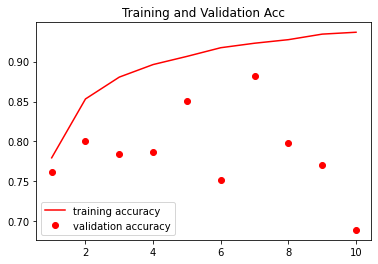
\includegraphics[width=1\textwidth,height=5cm,keepaspectratio]{Images/ResNet50V2BaselineTrainingValidationAccuracyExtensiveXray.png}\\
    \caption{Transfer Learning ResNet50V2 CNN Baseline Train and Validation Accuracy Extensive COVID 19 Dataset X-ray - The X-Axis shows the epoch number and the Y-axis shows the accuracy}
    \label{fig:ResNet50V2 CNN Baseline Train and Validation Accuracy Extensive COVID 19 Dataset X-ray}
\end{figure}
 \begin{figure}[H]
    \centering   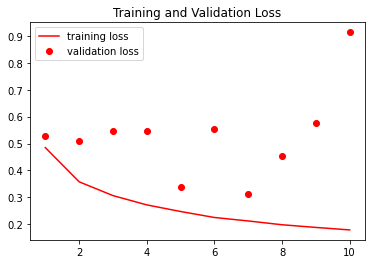
\includegraphics[width=1\textwidth,height=5cm,keepaspectratio]{Images/ResNet50V2BaselineTrainingValidationLossExtensiveXray.png}\\
    \caption{Transfer Learning ResNet50V2 CNN Baseline Train and Validation Loss Extensive COVID 19 Dataset X-ray - The X-Axis shows the epoch number and the Y-axis shows the loss}
    \label{fig:ResNet50V2 CNN Baseline Train and Validation Loss Extensive COVID 19 Dataset X-ray}
\end{figure}
\subsubsection{EfficientNetV2S}
This model is comprised of 20,659,553 parameters in total including an additional layer of 256 neurons using ReLU activation and an output layer of 1 neuron using a sigmoid activation function.  The model was trained for a total of 10 epochs with 209 steps per epoch and uses RMSprop as an optimizer with a learning rate of $1\times10^{-3}$ and a momentum of $1\times10^{-3}$.  The model achieved a training accuracy of 0.9840 and a training loss of 0.0396 along with a validation accuracy of 0.9702 and a validation loss of 0.2095.  The model also has a test set accuracy of 0.9766 and a test set loss of 0.1513.  Figure \ref{fig:EfficientNetV2S CNN Baseline Train and Validation Accuracy Extensive COVID 19 Dataset Xray} shows the training and validation accuracy and figure \ref{fig:EfficientNetV2S CNN Baseline Train and Validation Loss Extensive COVID 19 Dataset X-ray} shows the training and validation loss.
 \begin{figure}[H]
    \centering    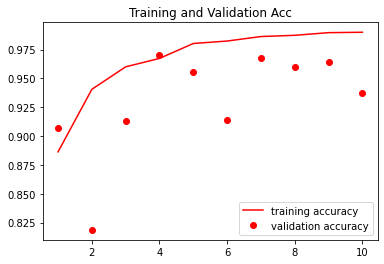
\includegraphics[width=1\textwidth,height=5cm,keepaspectratio]{Images/EfficientNetV2SBaselineTrainingValidationAccuracyExtensiveCT.png}\\
    \caption{Transfer Learning EfficientNetV2S CNN Baseline Train and Validation Accuracy Extensive COVID 19 Dataset X-ray - The X-Axis shows the epoch number and the Y-axis shows the accuracy}
    \label{fig:EfficientNetV2S CNN Baseline Train and Validation Accuracy Extensive COVID 19 Dataset Xray}
\end{figure}
 \begin{figure}[H]
    \centering
    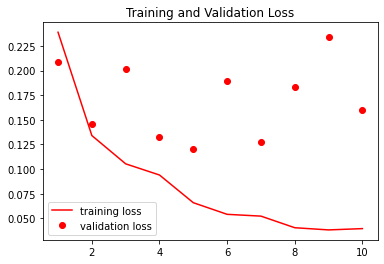
\includegraphics[width=1\textwidth,height=5cm,keepaspectratio]{Images/EfficientNetV2SBaselineTrainingValidationLossExtensiveXray.png}\\
    \caption{Transfer Learning EfficientNetV2S CNN Baseline Train and Validation Loss Extensive COVID 19 Dataset X-ray - The X-Axis shows the epoch number and the Y-axis shows the loss}
    \label{fig:EfficientNetV2S CNN Baseline Train and Validation Loss Extensive COVID 19 Dataset X-ray}
\end{figure}

\section{GAN Baseline Design and Comparison}
In this section we will detail the designs of the GANs and their architectures when augmenting classes in each database.  We will also compare the different results and effects each GAN architecture had when producing synthetic data.
\section{GANs for Radiography Dataset}
Due to a large imbalance between classes in the dataset we decided to explore the use of GANs to create synthetic data for both the COVID positive images which comprise 7,232 images in this dataset and the Pneumonia positive images which comprise 2,690 images.  The normal class (healthy patients) is very over-represented in the data as it is comprised of 20,384 images, due to this imbalance the CNNs trained from this dataset will be heavily biased towards identifying the normal patients.  For this reason we have chosen to use a number of Generative Adversarial Architectures to synthetically augment the classes lacking in data to balance the dataset and increase the generalization and robustness of the CNN models.
\subsection{VAE(Variational Auto Encoder)}
A few issues were encountered when running the variational auto encoder models for the radiography dataset.  When training on the masks we frequently ran into the issue of mode collapse, this is when the model only produces a single type of image.  Mode collapse occurred with both the COVID and Pneumonia datasets and can be seen below
 \begin{figure}[H]
    \centering
    
\includegraphics[width=1\textwidth,height=5cm,keepaspectratio]{Images/LatentSpace2VAECOVIDMask30Epochs.png}\\
    \caption{Example of Mode Collapse COVID Masks Radiography Dataset}
    \label{fig:Example of Mode Collapse COVID Masks Radiography Dataset}
\end{figure}
There were also issues faced when using a VAE on the X-ray data of both COVID and pneumonia images, the VAE tended to not produce any results when trained upon these X-rays and instead only showed a blank grid as output.  After a number of attempts to train both models it was found that the mask model suffered greatly from mode collapse and the X-ray model failed to produce any results for either class.
\subsection{DCGAN(Deep Convolutional GAN Network)}
\subsubsection{COVID-19 Mask Class Augmentation}
When designing the DCGAN we experimented with a number of architectures, some of these architectures led to the GAN only producing black squares which was a sign of mode collapse.  Mode collapse occurs when the discriminator gets stuck at a local minimum and the generator learns to only produce the same type of image over and over again to fool the discriminator. We found switching from an ADAM optimizer to RMSPROP and experimenting with the learning rate and momentum led to far better results.  The model produced some promising results, the following architecture was used to create the generator and discriminator:
\begin{minted}[linenos,tabsize=2,breaklines]{JavaScript}
# based off example: https://keras.io/examples/generative/dcgan_overriding_train_step/
discriminator = keras.Sequential(
    [
        keras.Input(shape=(128, 128, 3)),
        layers.Conv2D(64, kernel_size=4, strides=2, padding="same"),
        layers.LeakyReLU(alpha=0.5),
        layers.Conv2D(128, kernel_size=4, strides=2, padding="same"),
        layers.LeakyReLU(alpha=0.5),
        layers.Conv2D(128, kernel_size=4, strides=2, padding="same"),
        layers.LeakyReLU(alpha=0.5),
        layers.Flatten(),
        layers.Dropout(0.2),
        layers.Dense(1, activation="sigmoid"),
    ],
    name="discriminator",
)
discriminator.summary()

# Create the generator.
generator = keras.Sequential(
    [
        keras.Input(shape=(latent_dim,)),
        layers.Dense(8 * 8 * 128),
        layers.Reshape((8, 8, 128)),
        layers.Conv2DTranspose(256, kernel_size=4, strides=2, padding="same"),
        layers.LeakyReLU(alpha=0.2),
        layers.Conv2DTranspose(512, kernel_size=4, strides=2, padding="same"),
        layers.LeakyReLU(alpha=0.2),
        layers.Conv2DTranspose(1024, kernel_size=4, strides=2, padding="same"),
        layers.LeakyReLU(alpha=0.2),
        layers.Conv2DTranspose(64, kernel_size=4, strides=2, padding="same"),
        layers.LeakyReLU(alpha=0.2),
        layers.Conv2D(3, kernel_size=5, padding="same", activation="sigmoid"),
    ],
    name="generator",
)
generator.summary()
\end{minted}
The design of this GAN was based off of a Keras tutorial and the code was refactored for the purposes of this project\cite{DCGANKerasTutorial}.  The following hyper parameters were used when training the DCGAN model to generate synthetic COVID-19 mask images: 
\begin{table}[H]
    \centering
    \begin{tabular}{|c|c|}
    \hline
        Parameter
        & Value\\
         \hline
          Latent Dimension & 100\\
          Generator Optimizer & RMSProp \\
          Discriminator Optimizer & RMSProp\\
          Generator Learning Rate & $1\times10^{-5}$\\
          Discriminator Learning Rate & $1\times10^{-5}$\\
          Generator Momentum & 0\\
          Discriminator Momentum & 0\\
          Steps per Epoch & 452\\
          Batch Size & 8\\
          Number of Epochs & 100\\
         \hline
    \end{tabular}
    \caption{DCGAN for Producing Synthetic COVID-19 Mask Data From Radiography Dataset }
    \label{tab:DCGAN for Producing Synthetic COVID-19 Mask Data From Radiography Dataset}
\end{table}
With this model architecture we was able to achieve a final loss of 0.5476 for the discriminator and 1.0187 for the generator.
\subsubsection{COVID-19 X-Ray Class Augmentation}
Given the success achieved with the mask DCGAN we decided to reuse the architecture.  The results at first were blurry and had little resemblance to the actual data.  we decided to experiment with a number of different hyper parameters and found the parameters in the table below worked best:
\begin{table}[H]
    \centering
    \begin{tabular}{|c|c|}
    \hline
        Parameter
        & Value\\
         \hline
          Latent Dimension & 256\\
          Generator Optimizer & RMSProp \\
          Discriminator Optimizer & RMSProp\\
          Generator Learning Rate & $1\times10^{-5}$\\
          Discriminator Learning Rate & $1\times10^{-5}$\\
          Generator Momentum & 0\\
          Discriminator Momentum & 0\\
          Steps per Epoch & 452\\
          Batch Size & 8\\
          Number of Epochs & 100\\
         \hline
    \end{tabular}
    \caption{DCGAN for Producing Synthetic COVID-19 X-Ray Data From Radiography Dataset }
    \label{tab:DCGAN for Producing Synthetic COVID-19 X-Ray Data From Radiography Dataset}
\end{table}
With this model architecture we was able to achieve a final loss of 0.6859\% for the discriminator and 0.8015\% for the generator.
\subsubsection{Pneumonia Mask Class Augmentation}
The design of this DCGAN was based off the above COVID-19 DCGAN for generating masks and shares the same architecture the only difference being this model ran with 169 steps per epoch. The design yielded relatively similar results, although the losses for the pneumonia mask DCGAN was lower.  The model finished training with a loss of 0.9474 and a loss of 0.5936 for the discriminator.
\subsubsection{Pneumonia X-ray Class Augmentation}
The X-ray DCGAN for the pneumonia class is a copy of the above COVID-19 DCGAN the only difference being the Pneumonia X-Ray DCGAN uses a latent space of 256 and ran with 169 steps per epoch.  The model achieved a final loss of 0.6901 for the discriminator and a loss of 0.7534 for the generator.
\section{GANs for COVID 19 X-ray dataset}
\subsection{VAEs}
The decision was made not to train variational auto-encoders on this dataset given the poor performance of VAEs on the radiography dataset which is a lot larger than the X-ray COVID-19 dataset.  It appears that VAEs need much more data to train to recreate a similar image to the input data than the DCGAN models need.
\subsection{DCGANs}
There were some setbacks when training GANs on this dataset in particular due to the very limited amount of data it contained.  To remind the reader this dataset only contains 94 images of COVID-19 Positive X-Rays and 94 images of Pneumonia X-Rays.  When beginning the training of the GANs we merged both the train / test data for each class into two folders one marked Normal and the other marked Pneumonia each containing the 94 images of their respective class.  We merged both the test and the training data into the two files previously mentioned in order to utilize all the data available for augmenting the respective class. Most researchers suggest a minimum of 50k to 100k images to train a high quality GAN as mentioned on NVIDIAs website\cite{nvidiaResearch}. We attained some success with this DCGAN model surprisingly and augmented both the normal and pneumonia classes with 1,000 new images.
\\
The design of the DCGAN is as follows:
\begin{minted}[linenos,tabsize=2,breaklines]{JavaScript}
# based off example: https://keras.io/examples/generative/dcgan_overriding_train_step/
discriminator = keras.Sequential(
    [
        keras.Input(shape=(128, 128, 3)),
        layers.Conv2D(64, kernel_size=4, strides=2, padding="same"),
        layers.LeakyReLU(alpha=0.5),
        layers.Conv2D(128, kernel_size=4, strides=2, padding="same"),
        layers.LeakyReLU(alpha=0.5),
        layers.Conv2D(128, kernel_size=4, strides=2, padding="same"),
        layers.LeakyReLU(alpha=0.5),
        layers.Flatten(),
        layers.Dropout(0.4),
        layers.Dense(1, activation="sigmoid"),
    ],
    name="discriminator",
)
discriminator.summary()

# Create the generator.
generator = keras.Sequential(
    [
        keras.Input(shape=(latent_dim,)),
        layers.Dense(8 * 8 * 128),
        layers.Reshape((8, 8, 128)),
        layers.Conv2DTranspose(256, kernel_size=4, strides=2, padding="same"),
        layers.LeakyReLU(alpha=0.2),
        layers.Conv2DTranspose(512, kernel_size=4, strides=2, padding="same"),
        layers.LeakyReLU(alpha=0.2),
        layers.Conv2DTranspose(1024, kernel_size=4, strides=2, padding="same"),
        layers.LeakyReLU(alpha=0.2),
        layers.Conv2DTranspose(2048, kernel_size=4, strides=2, padding="same"),
        layers.LeakyReLU(alpha=0.2),
        layers.Conv2D(3, kernel_size=4, padding="same", activation="tanh"),
    ],
    name="generator",
)
generator.summary()

\end{minted}
The following hyper parameters were used to train the DCGAN to produce images from the normal class of the dataset
\begin{table}[H]
    \centering
    \begin{tabular}{|c|c|}
    \hline
        Parameter
        & Value\\
         \hline
          Latent Dimension & 256\\
          Generator Optimizer & RMSProp \\
          Discriminator Optimizer & RMSProp\\
          Generator Learning Rate & $1\times10^{-4}$\\
          Discriminator Learning Rate & $1\times10^{-4}$\\
          Generator Momentum & 0\\
          Discriminator Momentum & 0\\
          Steps per Epoch & 47\\
          Batch Size & 2\\
          Number of Epochs & 100\\
         \hline
    \end{tabular}
    \caption{DCGAN for Producing Synthetic Normal Class Data for X-ray COVID19 dataset}
    \label{tab:DCGAN for Producing Synthetic Normal Class Data for X-ray COVID19 dataset}
\end{table}
The final model achieved a loss of 0.6890 for the discriminator and a loss of 0.7623 for the generator.
\\
The augmentation of the pneumonia class had similar results as the normal class.  Given the success of the DCGAN architecture for the normal class it made sense to reuse this architecture when designing the DCGAN for the pneumonia class, the model also shares the same hyper-parameters.  The final model had a discriminator loss of 0.6895 and a generator loss of 0.7757 which is roughly around the same as the DCGAN for the normal class.
\section{GANs for Chest X-ray COVID-19}
Due to this model having 11 classes and limited data for each class a decision was made to exclude this dataset from the research.  This decision was made to conserve computational units and due to the limited data for each class.  There are also a number of classes in this dataset which contain very little data and are grossly underrepresented, the data for these classes is extremely limited and it would not be worthwhile training a GAN using this data.
\section{Extensive COVID-19 X-Ray / CT}
\subsection{VAEs}
The Extensive VAEs were trained on using both the X-ray COVID positive class and the Non-COVID CT class.  The output seemed to be fairly similar and it appears that the models suffered from mode collapse, but these images may have shown some benefit to the models.  The decision to conserve computational limits was made and the models were not augmented with data from the VAE models.  We have included images of the VAE models latent space below, as shown from the grids the resemblance between the images is striking although there may have been subtle differences non-descernible to the untrained eye.
 \begin{figure}[H]
    \centering
    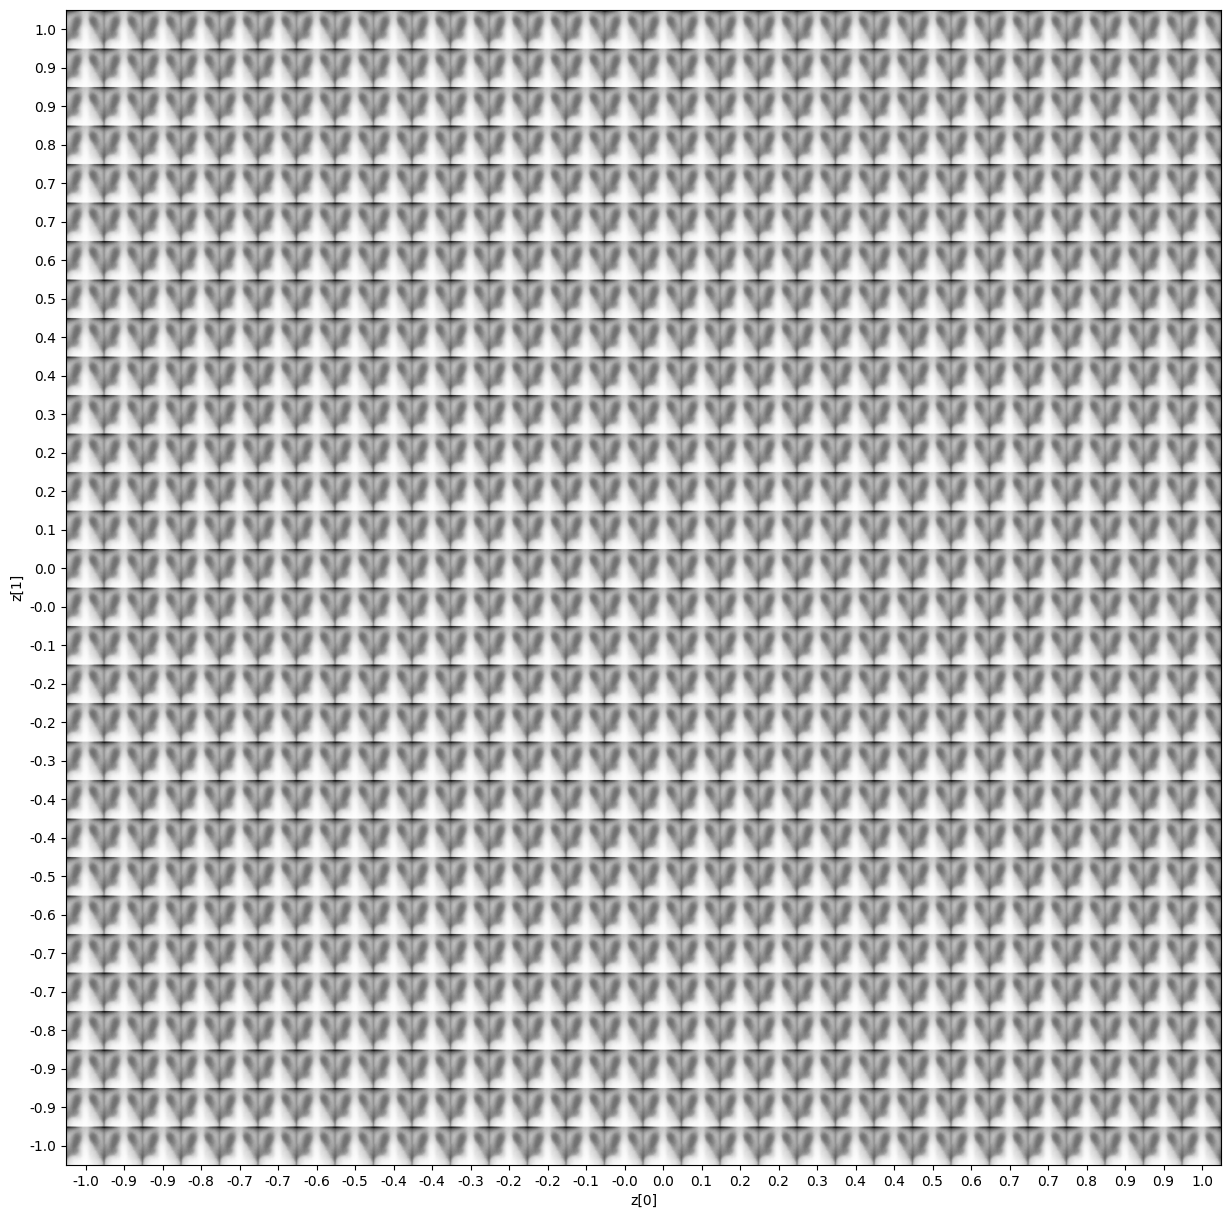
\includegraphics[width=1\textwidth,height=5cm,keepaspectratio]{Images/LatentSpaceExtensiveCOVIDXRay.png}\\
    \caption{Possible Mode Collapse COVID X-ray Extensive Dataset}
    \label{fig:Possible Mode Collapse COVID X-ray Extensive Dataset}
\end{figure}
 \begin{figure}[H]
    \centering
    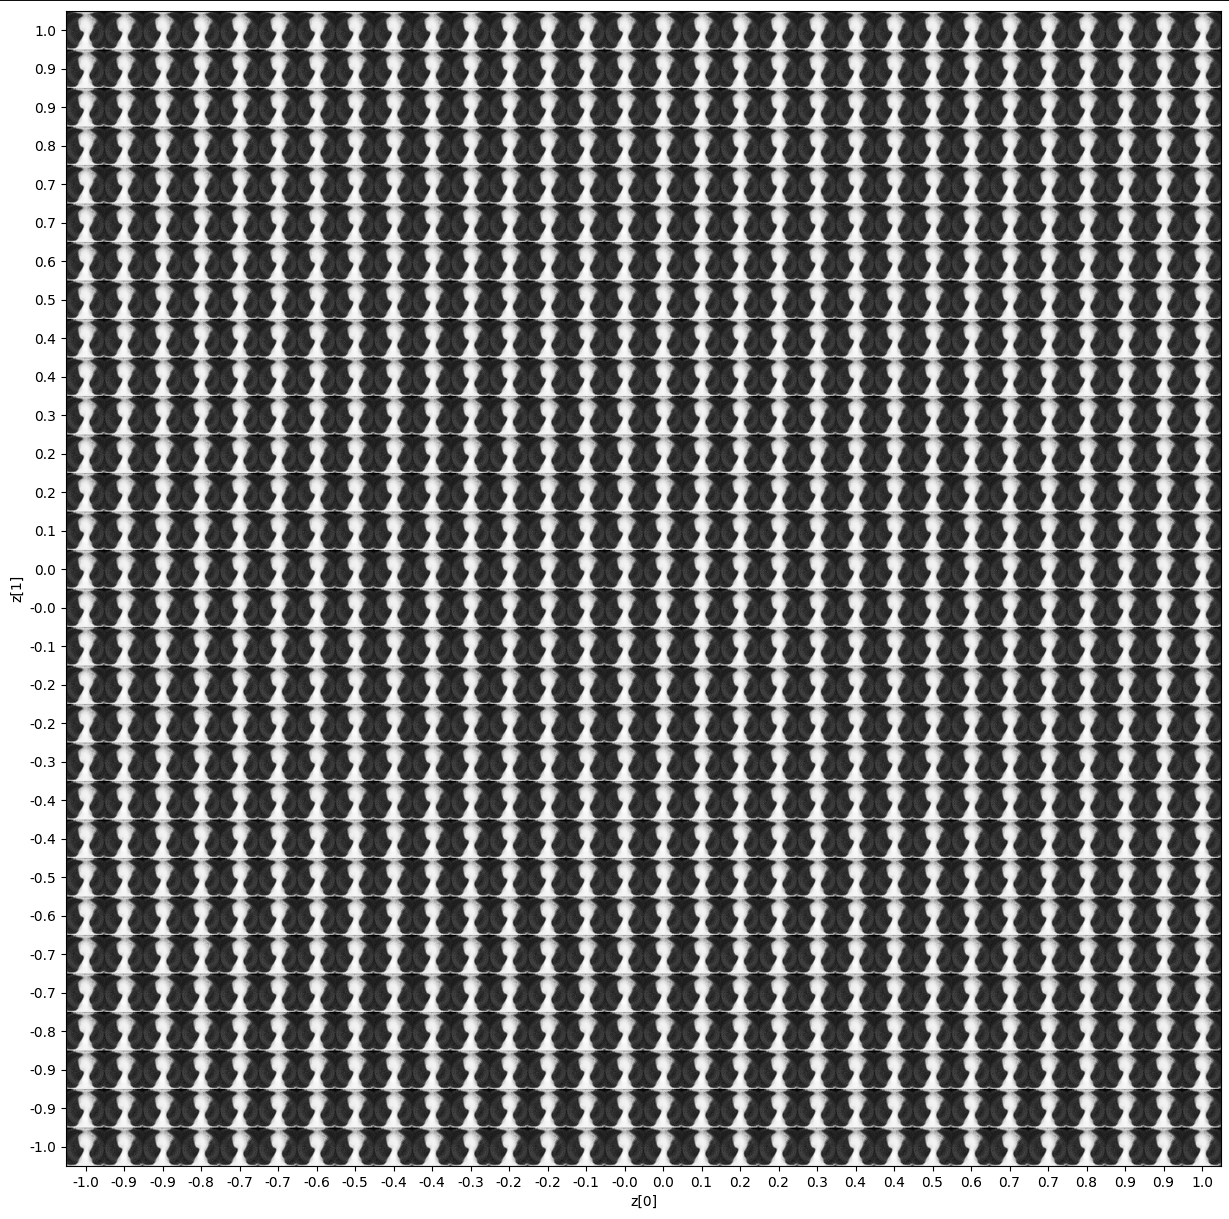
\includegraphics[width=1\textwidth,height=5cm,keepaspectratio]{Images/LatentSpaceExtensiveNonCovidCT.png}\\
    \caption{Possible Mode Collapse Non-Covid CT Extensive Dataset}
    \label{fig:Possible Mode Collapse Non-Covid CT Extensive Dataset}
\end{figure}
\subsection{DCGANs}
\subsubsection{X-ray DCGANs}
The extensive COVID-19 X-ray models were broken up into two classes COVID and Non-COVID.  The first model trained was trained to produce synthetic COVID images and ran for a total of 200 epochs and used the following architecture
\begin{minted}[linenos,tabsize=2,breaklines]{JavaScript}
# based off example: https://keras.io/examples/generative/dcgan_overriding_train_step/
discriminator = keras.Sequential(
    [
        keras.Input(shape=(128, 128, 3)),
        layers.Conv2D(64, kernel_size=4, strides=2, padding="same"),
        layers.LeakyReLU(alpha=0.5),
        layers.Conv2D(128, kernel_size=4, strides=2, padding="same"),
        layers.LeakyReLU(alpha=0.5),
        layers.Conv2D(128, kernel_size=4, strides=2, padding="same"),
        layers.LeakyReLU(alpha=0.5),
        layers.Flatten(),
        layers.Dropout(0.4),
        layers.Dense(1, activation="sigmoid"),
    ],
    name="discriminator",
)
discriminator.summary()

# Create the generator.
generator = keras.Sequential(A
    [
        keras.Input(shape=(latent_dim,)),
        layers.Dense(8 * 8 * 128),
        layers.Reshape((8, 8, 128)),
        layers.Conv2DTranspose(128, kernel_size=4, strides=2, padding="same"),
        layers.LeakyReLU(alpha=0.3),
        layers.Conv2DTranspose(256, kernel_size=4, strides=2, padding="same"),
        layers.LeakyReLU(alpha=0.3),
        layers.Conv2DTranspose(512, kernel_size=4, strides=2, padding="same"),
        layers.LeakyReLU(alpha=0.3),
        layers.Conv2DTranspose(1024, kernel_size=4, strides=2, padding="same"),
        layers.LeakyReLU(alpha=0.3),
        layers.Conv2D(3, kernel_size=4, padding="same", activation="tanh"),
    ],
    name="generator",
)
generator.summary()
\end{minted}
along with the following hyper parameters
\begin{table}[H]
    \centering
    \begin{tabular}{|c|c|}
    \hline
        Parameter
        & Value\\
         \hline
          Latent Dimension & 256\\
          Generator Optimizer & RMSProp \\
          Discriminator Optimizer & RMSProp\\
          Generator Learning Rate & $1\times10^{-4}$\\
          Discriminator Learning Rate & $1\times10^{-4}$\\
          Generator Momentum & 0\\
          Discriminator Momentum & 0\\
          Steps per Epoch & 253\\
          Batch Size &  16\\
          Number of Epochs & 200 \\
         \hline
    \end{tabular}
    \caption{DCGAN for Producing Synthetic X-ray COVID Class Data for Extensive COVID 19 Dataset}
    \label{tab:DCGAN for Producing Synthetic X-ray COVID Class Data for Extensive COVID 19 Dataset}
\end{table}
Once training finished the model attained a discriminator loss of 0.6901 and a generator loss of 0.7557.
\\ 
The next DCGAN architecture produced the Non-COVID class, this is the majority class but we wanted to compare and contrast the results from both DCGANs.  The model uses the following architecture 
\begin{minted}[linenos,tabsize=2,breaklines]{JavaScript}
# based off example: https://keras.io/examples/generative/dcgan_overriding_train_step/
discriminator = keras.Sequential(
    [
        keras.Input(shape=(128, 128, 3)),
        layers.Conv2D(64, kernel_size=4, strides=2, padding="same"),
        layers.LeakyReLU(alpha=0.5),
        layers.Conv2D(128, kernel_size=4, strides=2, padding="same"),
        layers.LeakyReLU(alpha=0.5),
        layers.Conv2D(128, kernel_size=4, strides=2, padding="same"),
        layers.LeakyReLU(alpha=0.5),
        layers.Flatten(),
        layers.Dropout(0.4),
        layers.Dense(1, activation="sigmoid"),
    ],
    name="discriminator",
)
# Create the generator.
generator = keras.Sequential(
    [
        keras.Input(shape=(latent_dim,)),
        layers.Dense(16 * 16 * 128),
        layers.Reshape((16, 16, 128)),
        layers.Conv2DTranspose(256, kernel_size=4, strides=2, padding="same"),
        layers.LeakyReLU(alpha=0.2),
        layers.Conv2DTranspose(512, kernel_size=4, strides=2, padding="same"),
        layers.LeakyReLU(alpha=0.2),
        layers.Conv2DTranspose(1024, kernel_size=4, strides=2, padding="same"),
        layers.LeakyReLU(alpha=0.2),
        layers.Conv2D(3, kernel_size=4, padding="same", activation="tanh"),
    ],
    name="generator",
)
\end{minted}
The model runs for 100 epochs and uses a learning rate of $10^{-5}$ for the generator and discriminator instead of $10^{-4}$.  The batch size was also increased to 64 to help the model train faster.  The model achieved a final loss of 0.6912 for the discriminator and 0.7575 for the generator.
\subsubsection{CT DCGANs}
For the DCGAN for CT Covid the batch size was chosen as 64 to increase the training speed.  The following architecture was used for this DCGAN
\begin{minted}[linenos,tabsize=2,breaklines]{JavaScript}
# based off example: https://keras.io/examples/generative/dcgan_overriding_train_step/
discriminator = keras.Sequential(
    [
        keras.Input(shape=(128, 128, 3)),
        layers.Conv2D(64, kernel_size=4, strides=2, padding="same"),
        layers.LeakyReLU(alpha=0.5),
        layers.Conv2D(128, kernel_size=4, strides=2, padding="same"),
        layers.LeakyReLU(alpha=0.5),
        layers.Conv2D(128, kernel_size=4, strides=2, padding="same"),
        layers.LeakyReLU(alpha=0.5),
        layers.Flatten(),
        layers.Dropout(0.4),
        layers.Dense(1, activation="sigmoid"),
    ],
    name="discriminator",
)
discriminator.summary()

# Create the generator.
generator = keras.Sequential(
    [
        keras.Input(shape=(latent_dim,)),
        layers.Dense(8 * 8 * 128),
        layers.Reshape((8, 8, 128)),
        layers.Conv2DTranspose(128, kernel_size=4, strides=2, padding="same"),
        layers.LeakyReLU(alpha=0.2),
        layers.Conv2DTranspose(256, kernel_size=4, strides=2, padding="same"),
        layers.LeakyReLU(alpha=0.2),
        layers.Conv2DTranspose(512, kernel_size=4, strides=2, padding="same"),
        layers.LeakyReLU(alpha=0.2),
        layers.Conv2DTranspose(1024, kernel_size=4, strides=2, padding="same"),
        layers.LeakyReLU(alpha=0.2),
        layers.Conv2D(3, kernel_size=4, padding="same", activation="tanh"),
    ],
    name="generator",
)
generator.summary()
\end{minted}
and used the following hyper parameters
\begin{table}[H]
    \centering
    \begin{tabular}{|c|c|}
    \hline
        Parameter
        & Value\\
         \hline
          Latent Dimension & 256\\
          Generator Optimizer & RMSProp \\
          Discriminator Optimizer & RMSProp\\
          Generator Learning Rate & $1\times10^{-4}$\\
          Discriminator Learning Rate & $1\times10^{-4}$\\
          Generator Momentum & 0\\
          Discriminator Momentum & 0\\
          Steps per Epoch & 85\\
          Batch Size &  64\\
          Number of Epochs & 100 \\
         \hline
    \end{tabular}
    \caption{DCGAN for Producing Synthetic CT COVID Class Data for Extensive COVID 19 Dataset}
    \label{tab:DCGAN for Producing Synthetic CT COVID Class Data for Extensive COVID 19 Dataset}
\end{table}
The model achieved a final loss score of 0.6443 for the discriminator and 0.9409 for the generator.
\\
The next model for the non-covid class uses the following architecture

\begin{minted}[linenos,tabsize=2,breaklines]{JavaScript}
# based off example: https://keras.io/examples/generative/dcgan_overriding_train_step/
discriminator = keras.Sequential(
    [
        keras.Input(shape=(128, 128, 3)),
        layers.Conv2D(64, kernel_size=4, strides=2, padding="same"),
        layers.LeakyReLU(alpha=0.5),
        layers.Conv2D(128, kernel_size=4, strides=2, padding="same"),
        layers.LeakyReLU(alpha=0.5),
        layers.Conv2D(128, kernel_size=4, strides=2, padding="same"),
        layers.LeakyReLU(alpha=0.5),
        layers.Flatten(),
        layers.Dropout(0.2),
        layers.Dense(1, activation="sigmoid"),
    ],
    name="discriminator",
)
discriminator.summary()

# Create the generator.
generator = keras.Sequential(
    [
        keras.Input(shape=(latent_dim,)),
        layers.Dense(4 * 4 * 128),
        layers.Reshape((4, 4, 128)),
        layers.Conv2DTranspose(64, kernel_size=4, strides=2, padding="same"),
        layers.LeakyReLU(alpha=0.2),
        layers.Conv2DTranspose(128, kernel_size=4, strides=2, padding="same"),
        layers.LeakyReLU(alpha=0.2),
        layers.Conv2DTranspose(256, kernel_size=4, strides=2, padding="same"),
        layers.LeakyReLU(alpha=0.2),
        layers.Conv2DTranspose(512, kernel_size=4, strides=2, padding="same"),
        layers.LeakyReLU(alpha=0.2),
        layers.Conv2DTranspose(1024, kernel_size=4, strides=2, padding="same"),
        layers.LeakyReLU(alpha=0.2),
        layers.Conv2D(3, kernel_size=4, padding="same", activation="tanh"),
    ],
    name="generator",
)
generator.summary()
\end{minted}
and the following hyper parameters 
\begin{table}[H]
    \centering
    \begin{tabular}{|c|c|}
    \hline
        Parameter
        & Value\\
         \hline
          Latent Dimension & 256\\
          Generator Optimizer & RMSProp \\
          Discriminator Optimizer & RMSProp\\
          Generator Learning Rate & $1\times10^{-4}$\\
          Discriminator Learning Rate & $1\times10^{-4}$\\
          Generator Momentum & 0\\
          Discriminator Momentum & 0\\
          Steps per Epoch & 42\\
          Batch Size &  64\\
          Number of Epochs & 100 \\
         \hline
    \end{tabular}
    \caption{DCGAN for Producing Synthetic CT Non COVID Class Data for Extensive COVID 19 Dataset}
    \label{tab:DCGAN for Producing Synthetic CT Non COVID Class Data for Extensive COVID 19 Dataset}
\end{table}
The model achieved a final loss score of 0.6522 for the discriminator and 1.0048 for the generator.
\section{Conclusion}
In conclusion most of the CNN models showed decent results when trained on the original datasets, although there are a few exceptions where the dataset used to train the models was small in size or imbalanced.  The GANs had achieved satisfactory results and produced images which were similar to those in the dataset which can be seen in the next chapter of this thesis.  Many of the models developed took a lot of tweaking, in order to get satisfactory results.  A lot of hyperparameter tuning was involved and the training was a time-consuming and laborious process as each model needed to be rerun when the hyperparameters were updated.
\\
With that said a number of models may benefit from more tweaking but for the purpose of this study the results achieved were satisfactory, given the purpose of this study is to gauge if synthetic data could improve an existing model's accuracy.  It is also worth remembering the models trained in this section are trained on limited data and/or imbalanced datasets which could skew the results. 


\chapter{Results}
\section{Evaluation of Performance of The Augmented CNN Models}
In this section we will evaluate the augmented CNN models and compare and contrast with the original models.  The section is broken into subsections for each datasets CNN models.
\subsection{Radiography CNN Models}
  The non-augmented radiography dataset was imbalanced so a total of 6,570 images were generated for the COVID X-rays and masks and a total of 8,840 pneumonia X-ray and mask images were generated to bring both classes in relative balance with the Normal class.  The augmented dataset will be off by a around 5-10 images for augmented classes due to computational issues when trying to generate all files at once but the results still show a big improvement in some models.  The augmented dataset contains 60,933, while the original dataset contained only 30,306. 
\subsubsection{Radiography Baseline Model}
The radiography baseline model ran for 10 epochs with 1333 steps per epoch and attained a final training set accuracy of 0.9314 and a final training set loss of 0.1663 along with a final validation set accuracy of 0.9200 and a validation set loss of 0.2200.  The  model achieved a test set accuracy of 0.9222 and a test set loss of 0.2068 when the dataset was augmented.  In comparison to the original model which has a training set accuracy of 0.8611 and a training loss of 0.3446 and a validation set accuracy of  0.8306 and a validation set loss of 0.4120 and a test set accuracy of 0.8434 and a test set loss of 0.3801  when trained for the same amount of epochs on the non-augmented set. The model trained on the augmented set shows a clear improvement in terms of accuracy and of loss.  The training accuracy increased by 0.0703 and the training loss decreased by 0.1683 along with the validation accuracy increasing by 0.0894 and the loss decreased by 0.192. The test set accuracy also increased by 0.0788 and the test set loss was lowered by 0.1732 when training on the augmented dataset.  In this case the augmented model shows a clear improvement over the original baseline model. The training and validation accuracy along with the training and validation loss of this model are shown below.
 \begin{figure}[H]
    \centering    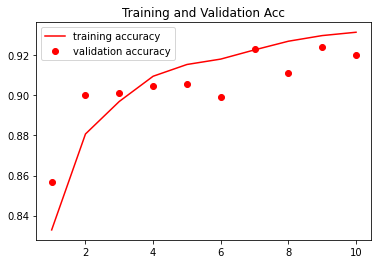
\includegraphics[width=1\textwidth,height=5cm,keepaspectratio]{Images/RadiographyCNNBaselineTrainAndValAccAugmentedDCGAN.png}\\
    \caption{Radiography Augmented Baseline Model DCGAN Accuracy - The X-Axis shows the epoch number and the Y-axis shows the accuracy}
    \label{fig:Radiography Augmented Baseline Model DCGAN Accuracy}
\end{figure}
 \begin{figure}[H]
    \centering
    \includegraphics[width=1\textwidth,height=5cm,keepaspectratio]{Images/RadiographyCNNBaselineTrainAndValLossAugmentedDCGAN.png}\\
    \caption{Radiography Augmented Baseline Model DCGAN Loss - The X-Axis shows the epoch number and the Y-axis shows the loss}
    \label{fig:Radiography Augmented Baseline Model DCGAN Loss}
\end{figure}
\subsubsection{Radiography Xception Model}
The augmented Radiography Xception model attained a final training set accuracy of 0.9699 and a final training set loss of 0.0776 alongside a final validation accuracy of 0.9435 and a final validation loss of 0.1365 after 10 epochs.  The model also achieved a final test set accuracy of 0.9464 and a test set loss of 0.1369.  In comparison the original model attained a training set accuracy of 0.9543 and a training set loss of 0.1162  alongside a validation set accuracy of 0.8964 and a validation set loss of 0.3867.  The original model also had a test set accuracy of 0.9002 and a test set loss of 0.3833.  The augmented model shows an increase of 0.0156 for the training accuracy and a decrease of 0.0386 for the training loss.  The validation set accuracy had an increase of 0.0471 and the validation set loss had an decrease of 0.2502. The model also performed better on the test set with accuracy increasing by 0.0462 and loss decreasing by 0.2464.  Again this model outperformed the original non-augmented model. Figure \ref{fig:Radiography Augmented Xception Model DCGAN Accuracy} shows the training and validation accuracy and figure \ref{fig:Radiography Augmented Xception Model DCGAN Loss} shows the training and validation loss.
 \begin{figure}[H]
    \centering    \includegraphics[width=1\textwidth,height=5cm,keepaspectratio]{Images/RadiographyCNNXceptionTrainAndValAccAugmentedDCGAN.png}\\
    \caption{Radiography Augmented Xception Model DCGAN Accuracy - The X-Axis shows the epoch number and the Y-axis shows the accuracy}
    \label{fig:Radiography Augmented Xception Model DCGAN Accuracy}
\end{figure}
 \begin{figure}[H]
    \centering
    \includegraphics[width=1\textwidth,height=5cm,keepaspectratio]{Images/RadiographyCNNXceptionTrainAndValLossAugmentedDCGAN.png}\\
    \caption{Radiography Augmented Xception Model DCGAN Loss - The X-Axis shows the epoch number and the Y-axis shows the loss}
    \label{fig:Radiography Augmented Xception Model DCGAN Loss}
\end{figure}
\subsubsection{Radiography ResNet50V2 Model}
The augmented radiography ResNet50V2 Model attained a final training set accuracy of 0.9593 and a training set loss of 0.1034 alongside a validation set accuracy of 0.8638 and a validation set loss of 0.3838.  The augmented model also has a test set accuracy of 0.8623 and a test set loss of 0.3814.  To contrast this with the original model, the original model attained a final training set accuracy of 0.9172 and a training set loss of 0.2024 along with a validation set accuracy of 0.8695 and a validation set loss of 0.3944.  The original model also had a test set accuracy of 0.8809 and a test set loss of 0.3942.  The augmented model performs better on the training set with an accuracy increase of 0.0421 and a loss decrease of 0.099 but performed worse on the validation set in terms of accuracy with an accuracy decrease of 0.0057 and a loss decrease of 0.0106.   The model also performed slightly worse on the test set in terms of accuracy with a decrease of 0.0186 although it did have a decrease in loss which decreased by 0.0129. Figure \ref{fig:Radiography Augmented ResNet50V2 Model DCGAN Accuracy} shows the training and validation accuracy and figure \ref{fig:Radiography Augmented ResNet50V2 Model DCGAN Loss} shows the training and validation loss.
 \begin{figure}[H]
    \centering    
    \includegraphics[width=1\textwidth,height=5cm,keepaspectratio]{Images/RadiographyCNNResNet50V2TrainAndValAccAugmentedDCGAN.png}\\
    \caption{Radiography Augmented ResNet50V2 Model DCGAN Accuracy - The X-Axis shows the epoch number and the Y-axis shows the accuracy}
    \label{fig:Radiography Augmented ResNet50V2 Model DCGAN Accuracy}
\end{figure}
 \begin{figure}[H]
    \centering
    \includegraphics[width=1\textwidth,height=5cm,keepaspectratio]{Images/RadiographyCNNResNet50V2TrainAndValLossAugmentedDCGAN.png}\\
    \caption{Radiography Augmented ResNet50V2 Model DCGAN Loss - The X-Axis shows the epoch number and the Y-axis shows the loss}
    \label{fig:Radiography Augmented ResNet50V2 Model DCGAN Loss}
\end{figure}
\subsubsection{Radiography EfficentNetV2S Model}
The augmented EfficentNetV2S Model completed training with a final training set accuracy of 0.9640, with a training set loss of 0.0910 alongside a validation set accuracy of 0.9553 and a validation loss of 0.1167.  The model also had a test set accuracy of 0.9604 and a test set loss of 0.1056.  In contrast the original model attained a final training set accuracy 0.9383  of and a training set loss of 0.1519 alongside a validation accuracy of 0.8844 and a validation loss of 0.3362.  The original model also achieved a test set accuracy of 0.8811 and a test set loss of 0.3217.  This shows that the augmented model's training set accuracy increased by 0.0257 and its training set loss decreased by 0.0609 and the validation set accuracy increased by 0.0709 and its validation loss decreased by 0.2195.  The test set also improved in terms of loss and accuracy with an accuracy increase of 0.0794 and a loss decrease of 0.2161.   The augmented model has shown clear improvements when compared with the base model however, as shown from the images below early stopping could have helped improve the accuracy for the validation set. Figure \ref{fig:Radiography Augmented EfficientNetV2S Model DCGAN Accuracy} shows the training and validation accuracy and figure \ref{fig:Radiography Augmented EfficientNetV2S Model DCGAN Loss} shows the training and validation loss.
 \begin{figure}[H]
    \centering    \includegraphics[width=1\textwidth,height=5cm,keepaspectratio]{Images/EfficientNetV2SBaselineTrainingValidationAccRadiographyAugmentedDCGAN.png}\\
    \caption{Radiography Augmented EfficientNetV2S Model DCGAN Accuracy The X-Axis shows the epoch number and the Y-axis shows the accuracy} 
    \label{fig:Radiography Augmented EfficientNetV2S Model DCGAN Accuracy}
\end{figure}
 \begin{figure}[H]
    \centering
    \includegraphics[width=1\textwidth,height=5cm,keepaspectratio]{Images/EfficientNetV2SBaselineTrainingValidationLossRadiographyAugmentedDCGAN.png}\\
    \caption{Radiography Augmented EfficientNetV2S Model DCGAN Loss - The X-Axis shows the epoch number and the Y-axis shows the loss}
    \label{fig:Radiography Augmented EfficientNetV2S Model DCGAN Loss}
\end{figure}
\subsubsection{Evaluation of Radiography Models}
Most of the radiography models showed a clear improvement across all sets when training on the augmented datasets.  The models which performed worse only suffered from a slight decrease in performance in terms of accuracy but had a decrease in loss which means the model may not have predicted all the cases correctly but was more confident in doing so.  The increase in confidence of all the radiography models could avoid situations where patients are unnecessarily quarantined.  The results from this dataset are significant in that they show a clear improvement across all models.
\subsection{Extensive CNN Models}
The Extensive CT dataset was augmented by 2,700 images and the augmented dataset has a total of 10,754 images, the original Extensive CT dataset had 8,054 images.  The original Extensive X-ray dataset had a total of 9,537 images which was increased to 10,537 when augmented, in total an additional 1,180 images were added to the augmented dataset.
\subsubsection{Extensive CNN CT Baseline Model}
The Extensive CNN CT baseline model attained a final training set accuracy of 0.9199 and a final training set loss of 0.1839 along with a final validation set accuracy of 0.5333 and a validation set loss of 3.4314  when the dataset was augmented.  The model  also had a test set loss of 3.2788  and a test set accuracy of  0.5373. In comparison to the original model which had a training set accuracy of 0.9023 and a training set loss of 0.2286 and a validation set accuracy of 0.8150 and a validation set loss of 0.3837  when trained for the same amount of epochs on a non-augmented set.  The original model also had a test set accuracy of 0.8319 and a test set loss of 0.3574.  Overall the augmented model performed better on the training set but worse on both the validation and test sets.  The training set accuracy increased by 0.0176 and the training set loss decreased by 0.0447 along with the validation set accuracy decreasing by 0.2817 and the loss increasing by 3.0477. The test set accuracy also declined by 0.2946 and the loss increased by 2.9206.  The training and validation set accuracy along with the training and validation set loss of this model are shown below.  The model appears to have a significant decrease in accuracy on the 10th epoch early stopping may have improved the overall accuracy.  Figure \ref{fig:Extensive CT Augmented Baseline Model DCGAN Accuracy} shows the training and validation accuracy and figure \ref{fig:Extensive CT Augmented Baseline Model DCGAN Loss} shows the training and validation loss.
 \begin{figure}[H]
    \centering    \includegraphics[width=1\textwidth,height=5cm,keepaspectratio]{Images/ExtensiveCNNBaselineModelExtensiveCovidAccCTAugmentedDCGAN.png}\\
    \caption{Extensive CT Augmented Baseline Model DCGAN Accuracy - The X-Axis shows the epoch number and the Y-axis shows the accuracy}
    \label{fig:Extensive CT Augmented Baseline Model DCGAN Accuracy}
\end{figure}
 \begin{figure}[H]
    \centering
    \includegraphics[width=1\textwidth,height=5cm,keepaspectratio]{Images/ExtensiveCNNBaselineModelExtensiveCovidLossCTAugmentedDCGAN.png}\\
    \caption{Extensive CT Augmented Baseline Model DCGAN - The X-Axis shows the epoch number and the Y-axis shows the loss}
    \label{fig:Extensive CT Augmented Baseline Model DCGAN Loss}
\end{figure}
\subsubsection{Extensive CNN CT Xception Model}
The Extensive CNN CT Xception model attained a final training set accuracy of 0.9920 and a final training set loss of 0.0278 along with a final validation set accuracy of 0.9704 and a validation set loss of 0.0777 when the dataset was augmented.  The model also has a test set accuracy of 0.9688 and a test set loss of 0.1054.  In comparison to the original model which had a training set accuracy of 0.9904  and a training set loss of 0.0238 and a validation set accuracy of 0.9534 and a validation set loss of 0.2250 when trained for the same amount of epochs on a non-augmented set.  The original model also had a test set accuracy of 0.9538 and a test set loss of 0.1772.  The augmented model performed better on all sets.  The training set accuracy increased by 0.0016 and the training set loss decreased by 0.1494. The validation set accuracy increased by 0.017 and the loss decreased by 0.1472. The test set accuracy also increased by 0.015 and the test set loss decreased by 0.0717.  Early stopping would have improved accuracy on the validation set as shown in the figures below which may in turn have improved the test set accuracy.  Figure \ref{fig:Extensive CT Augmented Xception Model DCGAN Accuracy} shows the training and validation accuracy and figure \ref{fig:Extensive CT Augmented Xception Model DCGAN Loss} shows the training and validation loss.
 \begin{figure}[H]
    \centering    \includegraphics[width=1\textwidth,height=5cm,keepaspectratio]{Images/XceptionBaselineTrainingValidationAccuracyExtensiveCTAugmentedDCGAN.png}\\
    \caption{Extensive CT Augmented Xception Model DCGAN Accuracy - The X-Axis shows the epoch number and the Y-axis shows the accuracy}
    \label{fig:Extensive CT Augmented Xception Model DCGAN Accuracy}
\end{figure}
 \begin{figure}[H]
    \centering
    \includegraphics[width=1\textwidth,height=5cm,keepaspectratio]{Images/XceptionBaselineTrainingValidationLossExtensiveCTAugmentedDCGAN.png}\\
    \caption{Extensive CT Augmented Xception Model DCGAN Loss - The X-Axis shows the epoch number and the Y-axis shows the loss}
    \label{fig:Extensive CT Augmented Xception Model DCGAN Loss}
\end{figure}
\subsubsection{Extensive CNN CT ResNet50V2 Model}
The Extensive CNN CT ResNet50V2 model attained a final training set accuracy of 0.9485 and a final training set loss of 0.1255 along with a final validation set accuracy of 0.6091 and a validation set loss of 1.1563 when the dataset was augmented.  The model also has a test set accuracy of 0.6040 and a test set loss of 1.1806.  In comparison to the original model which had a training set accuracy of 0.9604 and a training set loss of 0.1140 and a validation set accuracy of 0.9350 and a validation set loss of 0.2078  when trained for the same amount of epochs on a non-augmented set.  The original model also had a test set accuracy of 0.9262 and a test set loss of 0.1993.  The augmented model performed worse on all sets.  The training set accuracy decreased by 0.0119 and the training set loss increased by 0.0115. The validation set accuracy decreased by 0.3259 and the validation set loss increased by 0.9485. The test accuracy also decreased by 0.3222 and the test loss increased by 0.9807.  Early stopping may have improved accuracy on the training and validation sets as shown in the figures below which may in turn have improved the test set accuracy.  Figure \ref{fig:Extensive CT Augmented ResNet50V2 Model DCGAN Accuracy} shows the training and validation accuracy and figure \ref{fig:Extensive CT Augmented ResNet50V2 Model DCGAN Loss} shows the training and validation loss.
 \begin{figure}[H]
    \centering    \includegraphics[width=1\textwidth,height=5cm,keepaspectratio]{Images/ResNet50V2BaselineTrainingValidationAccuracyExtensiveCTAugmentedDCGAN.png}\\
    \caption{Extensive CT Augmented ResNet50V2 Model DCGAN Accuracy - The X-Axis shows the epoch number and the Y-axis shows the accuracy}
    \label{fig:Extensive CT Augmented ResNet50V2 Model DCGAN Accuracy}
\end{figure}
 \begin{figure}[H]
    \centering
    \includegraphics[width=1\textwidth,height=5cm,keepaspectratio]{Images/ResNet50V2BaselineTrainingValidationLossExtensiveCTAugmentedDCGAN.png}\\
    \caption{Extensive CT Augmented ResNet50V2 Model DCGAN Loss - The X-Axis shows the epoch number and the Y-axis shows the loss}
    \label{fig:Extensive CT Augmented ResNet50V2 Model DCGAN Loss}
\end{figure}
\subsubsection{Extensive CNN CT EfficientNetV2S Model}
The Extensive CNN CT EfficientNetV2S model attained a final training set accuracy of 0.9957 and a final training set loss of 0.0150 along with a final validation accuracy of 0.9815 and a validation set loss of 0.0634  when the dataset was augmented.  The augmented model also has a test accuracy of 0.9790 and a test loss of 0.0874.  In comparison to the original model which had a training set accuracy of 0.9901 and a training set loss of 0.0291 and a validation set accuracy of 0.9375 and a validation set loss of 0.2638 when trained for the same amount of epochs on a non-augmented set.  The original model also has a test set accuracy of 0.9437 and a test set loss of 0.2353.  The model performed better on all sets when training on the augmented set.  The training accuracy increased by 0.0056 and the training loss decreased by 0.0141. The validation accuracy increased by 0.044 and the loss decreased by 0.2004.  The test set accuracy increased by 0.0352 and the test set loss decreased by 0.1479.  This is an improvement over the original model on all sets which is a significant result.  Figure \ref{fig:Extensive CT Augmented EfficientNetV2S Model DCGAN Accuracy} shows the training and validation accuracy and figure \ref{fig:Extensive CT Augmented EfficientNetV2S Model DCGAN Loss} shows the training and validation loss.

 \begin{figure}[H]
    \centering    \includegraphics[width=1\textwidth,height=5cm,keepaspectratio]{Images/EfficientNetV2STrainingValidationAccuracyExtensiveCTAugmentedDCGAN.png}\\
    \caption{Extensive CT Augmented EfficientNetV2S Model DCGAN Accuracy - The X-Axis shows the epoch number and the Y-axis shows the accuracy}
    \label{fig:Extensive CT Augmented EfficientNetV2S Model DCGAN Accuracy}
\end{figure}
 \begin{figure}[H]
    \centering
    \includegraphics[width=1\textwidth,height=5cm,keepaspectratio]{Images/EfficientNetV2SBaselineTrainingValidationLossExtensiveCT.png}\\
    \caption{Extensive CT Augmented EfficientNetV2S Model DCGAN - The X-Axis shows the epoch number and the Y-axis shows the loss}
    \label{fig:Extensive CT Augmented EfficientNetV2S Model DCGAN Loss}
\end{figure}
\subsubsection{Evaluation of Extensive CNN CT Models}
The extensive CT models had mixed results when training on the augmented set.  The baseline model performed worse as did the ResNet50V2 model although the Xception and EfficientNetV2S models showed improvements across all sets.  Early stopping may have improved the accuracy for the Baseline and ResNet50V2 models as shown in the figures showing the validation and training accuracy and losses, it appears that the models may have been overtrained when training for the same number of epochs as the original given there is more data in the augmented sets.  The baseline model shows clear signs of overtraining as there is a large loss in accuracy and a large increase in loss on the 10th epoch and the ResNet50V2 model shows a large drop in accuracy on the 10th epoch as well.
\subsubsection{Extensive CNN X-ray Baseline Model}
The Extensive CNN X-ray baseline model attained a final training set accuracy of 0.9257 and a final training set loss of 0.1911 along with a final validation set accuracy of 0.7741 and a validation set loss of 1.1363 when the dataset was augmented. The augmented model also had a test set accuracy of 0.7784 and a test set loss of 1.0640.  In comparison to the original model which had a training set accuracy of 0.9278 and a training set loss of 0.1948 in addition to a validation set accuracy of 0.8587 and a validation set loss of 0.3482  when trained for the same amount of epochs on a non-augmented set.  The original model also had a test set accuracy of 0.8698 and a test set loss of 0.3203.  The model performed worse on all sets when trained on the augmented set.  The training set accuracy decreased by 0.0021 and the training set loss decreased by 0.0037. The validation set accuracy decrease by 0.0846 and the validation set loss increased by 0.7881.  The test set accuracy decreased by 0.0914 and the test set loss increased by 0.7437.
 \begin{figure}[H]
    \centering    \includegraphics[width=1\textwidth,height=5cm,keepaspectratio]{Images/BaselineTrainingValidationAccuracyExtensiveXRayAugmentedDCGAN.png}\\
    \caption{Extensive X-ray Augmented Baseline Model DCGAN Accuracy - The X-Axis shows the epoch number and the Y-axis shows the accuracy}
    \label{fig:Extensive X-ray Augmented Baseline Model DCGAN Accuracy}
\end{figure}
 \begin{figure}[H]
    \centering
    \includegraphics[width=1\textwidth,height=5cm,keepaspectratio]{Images/BaselineTrainingValidationLossExtensiveXRayAugmentedDCGAN.png}\\
    \caption{Extensive X-ray Augmented Baseline Model DCGAN Loss - The X-Axis shows the epoch number and the Y-axis shows the loss}
    \label{fig:Extensive X-ray Baseline Model DCGAN Loss}
\end{figure}
\subsubsection{Extensive CNN X-ray Xception Model}
The Extensive CNN X-ray Xception model attained a final training set accuracy of 0.9864 and a final training set loss of 0.0304 along with a final validation set accuracy of 0.9581 and a validation set loss of 0.2502 when the dataset was augmented.  The augmented model also has a test set accuracy of 0.9659 and a test set loss of 0.2254.  In comparison to the original model which had a training set accuracy of 0.9876 and a training set loss of 0.0277 in addition to a validation set accuracy of 0.9416 and a validation set loss of 0.2814 when trained for the same amount of epochs on a non-augmented set.  The original model also has a test set accuracy of 0.9578 and a test set loss of 0.1948.  The model performed slightly worse on the training set but better on both the validation set and on the test set when training on the augmented set.  The training set accuracy decreased by 0.0012 and the training set loss increased by 0.0027. The validation set accuracy increased by 0.0165 and the validation set loss decreased by 0.0312.  The test set accuracy increased by 0.0081 and the test set loss increased by 0.0306. The augmented and original model are fairly close in terms of accuracy and loss with the augmented model performing worse on the training set by a small margin but the model performed better on the validation and test sets in terms of accuracy by a small margin although the loss for the test set is slightly higher in the augmented model. Figure \ref{fig:Extensive X-ray Augmented Xception Model DCGAN Accuracy} shows the training and validation accuracy and figure \ref{fig:Extensive X-ray Augmented Xception Model DCGAN Loss} shows the training and validation loss.
 \begin{figure}[H]
    \centering    \includegraphics[width=1\textwidth,height=5cm,keepaspectratio]{Images/XceptionBaselineTrainingValidationAccuracyExtensiveXray.png}\\
    \caption{Extensive X-ray Augmented Xception Model DCGAN Accuracy - The X-Axis shows the epoch number and the Y-axis shows the accuracy}
    \label{fig:Extensive X-ray Augmented Xception Model DCGAN Accuracy}
\end{figure}
 \begin{figure}[H]
    \centering
    \includegraphics[width=1\textwidth,height=5cm,keepaspectratio]{Images/XceptionBaselineTrainingValidationLossExtensiveXray.png}\\
    \caption{Extensive X-ray Augmented Xception Model DCGAN Loss - The X-Axis shows the epoch number and the Y-axis shows the loss}
    \label{fig:Extensive X-ray Augmented Xception Model DCGAN Loss}
\end{figure}
\subsubsection{Extensive CNN X-ray ResNet50V2 Model}
The Extensive CNN X-ray ResNet50V2 model attained a final training set accuracy of 0.9687 and a final training set loss of 0.0852 along with a final validation set accuracy of 0.8275 and a validation set loss of 0.4574 when the dataset was augmented.  The augmented model also achieved an accuracy of 0.8210 for the test set along with a test set loss of 0.4680.  In comparison to the original model which has a training set accuracy of 0.9649 and a training set loss of 0.0907 in addition to a validation set accuracy of 0.9139 and a validation set loss of 0.9139 when trained for the same amount of epochs on a non-augmented set.  The original model also had a test set accuracy of 0.9224 and a test set loss of 0.2379.  The model performed worse on all sets when training on the augmented set.  The training set accuracy decreased by 0.0038 and the training set loss decreased by 0.0055. The validation set accuracy decreased by 0.0864 and the validation set loss increased by 0.1732.  Test set accuracy decreased by 0.1014 and the test set loss increased by 0.2301.
 \begin{figure}[H]
    \centering    \includegraphics[width=1\textwidth,height=5cm,keepaspectratio]{Images/ResNet50V2BaselineTrainingValidationAccuracyExtensiveXray.png}\\
    \caption{Extensive X-ray Augmented ResNet50V2 Model DCGAN Accuracy - The X-Axis shows the epoch number and the Y-axis shows the accuracy}
    \label{fig:Extensive X-ray Augmented ResNet50V2 Model DCGAN Accuracy}
\end{figure}
 \begin{figure}[H]
    \centering
    \includegraphics[width=1\textwidth,height=5cm,keepaspectratio]{Images/ResNet50V2BaselineTrainingValidationLossExtensiveXrayAugmentedDCGAN.png}\\
    \caption{Extensive X-ray Augmented ResNet50V2 Model DCGAN Loss - The X-Axis shows the epoch number and the Y-axis shows the loss}
    \label{fig:Extensive X-ray Augmented ResNet50V2 Model DCGAN Loss}
\end{figure}
\subsubsection{Extensive CNN X-ray EfficientNetV2S Model}
The Extensive CNN X-ray EfficientNetV2S model attained a final training set accuracy of 0.9864 and a final training set loss of 0.0366 along with a final validation set accuracy of 0.9695 and a validation set loss of 0.1686 when the dataset was augmented.  The model also has a test set accuracy of 0.9697 and a test set loss of 0.1579.  In comparison to the original model which had a training set accuracy of 0.9840 and a training set loss of 0.0396 in addition to a validation set accuracy of 0.9702 and a validation set loss of 0.1603 when trained for the same amount of epochs on a non-augmented set.  The original model also has a test set accuracy of 0.9766 and a test set loss of 0.1513.  The model performed slightly worse on all sets except the training set when training on the augmented set.  The training set accuracy increased by 0.0024 and the training set loss decreased by 0.003. The validation set accuracy decreased by 0.0007 and the validation set loss increased by 0.0083.  The test set accuracy decreased by 0.0069 and the test set loss increased by 0.0066.  It appears from analyzing these models that the quality of the X-ray images don't match the quality of the CT images as all the X-ray models performed worse than the originals. Figure \ref{fig:Extensive X-ray Augmented EfficientNetV2S Model DCGAN Accuracy} shows the training and validation accuracy and figure \ref{fig:Extensive X-ray Augmented EfficientNetV2S Model DCGAN Loss} shows the training and validation loss.
 \begin{figure}[H]
    \centering    \includegraphics[width=1\textwidth,height=5cm,keepaspectratio]{Images/EfficientNetV2SBaselineTrainingValidationAccuracyExtensiveXRayAugmentedDCGAN.png}\\
    \caption{Extensive X-ray Augmented EfficientNetV2S Model DCGAN Accuracy - The X-Axis shows the epoch number and the Y-axis shows the accuracy}
    \label{fig:Extensive X-ray Augmented EfficientNetV2S Model DCGAN Accuracy}
\end{figure}
 \begin{figure}[H]
    \centering
    \includegraphics[width=1\textwidth,height=5cm,keepaspectratio]{Images/EfficientNetV2SBaselineTrainingValidationLossExtensiveXRayAugmentedDCGAN.png}\\
    \caption{Extensive X-ray Augmented EfficientNetV2S Model DCGAN Loss - The X-Axis shows the epoch number and the Y-axis shows the loss}
    \label{fig:Extensive X-ray Augmented EfficientNetV2S Model DCGAN Loss}
\end{figure}
\subsubsection{Evaluation of Extensive CNN X-ray Models}
Most of the Extensive X-ray CNN models performed worse in terms of accuracy and loss bar the Xception model which had slight improvements to both accuracy and loss.  The reason for the poor performance may be due to the variety in the X-ray images for this dataset as some X-rays are taken from the side and others are taken when the patient is facing forward. The poor performance could also have been caused by the quality of the augmented data.  When analyzing the output of the GAN for the X-ray model it appears that a lot of the images are grainy and lacking in quality.  The CT models on the other hand showed a clear improvement as the data generated from that set may suffer from grain and artifacts but the synthetic images share a lot of features with the original images.
\subsection{X-ray COVID-19 dataset CNN Models}
This dataset was augmented with 2000 artificially generated images, 1000 belonging to the pneumonia class and the other 1000 belonging to the normal class.  The augmented images were used only in training the models. Given the limited size of the dataset if we were to include augmented images in the validation set it would greatly skew the results as we would be gauging the model's ability to predict synthetic images as opposed to real images.  The limited size of the validation set for these models means that their performance is open to scrutiny.  The transfer learning models for this model include an additional layer of 1024 units with a ReLU activation function and another layer of 1 unit with a Sigmoid activation function.  The total size of the augmented set amounts to 2,148 images, the original dataset contained only 188 images. 
\subsubsection{X-ray COVID-19 Baseline Model}
The X-ray COVID-19 Baseline model attained a final training set accuracy of 0.9926 and a final training set loss of 0.0207 along with a final validation set accuracy of 0.5000 and a validation set loss of 5.2546 when the dataset was augmented.  The model also has a test set accuracy of 0.4375 and a test set loss of 6.2093.  In comparison to the original model which had a training set accuracy of 0.9122 and a training set loss of 0.2651 in addition to a validation set accuracy of 0.5000 and a validation set loss of 0.7918 when trained for the same amount of epochs on a non-augmented set.  The model performed worse on the validation and test sets in terms of accuracy when training on the augmented set but the augmented model had a higher accuracy and lower loss for the training set.  The training set accuracy increased by 0.0804 and the training set loss decreased by 0.2444. The validation set accuracy stayed the same at 0.5000 and the validation set loss increased by 4.4628.  The test set accuracy decreased by 0.0313 and the test set loss increased by 5.392.  Early stopping may have helped this model as the loss is a lot lower at epoch 8 and 9 for the validation set and has a higher validation accuracy with similar training accuracy.  Figure \ref{fig:X-ray COVID-19 Augmented Baseline Model DCGAN Accuracy} shows the training and validation accuracy and figure \ref{fig:X-ray COVID-19 Augmented Baseline Model DCGAN Loss} shows the training and validation loss.
 \begin{figure}[H]
    \centering    \includegraphics[width=1\textwidth,height=5cm,keepaspectratio]{Images/X-ray COVID-19 dataset CNN Train and Val Acc Augmented DCGAN.png}\\
    \caption{X-ray COVID-19 Augmented Baseline Model DCGAN Accuracy - The X-Axis shows the epoch number and the Y-axis shows the accuracy}
    \label{fig:X-ray COVID-19 Augmented Baseline Model DCGAN Accuracy}
\end{figure}
 \begin{figure}[H]
    \centering
    \includegraphics[width=1\textwidth,height=5cm,keepaspectratio]{Images/X-ray COVID-19 dataset CNN Train and Val Loss Augmented DCGAN.png}\\
    \caption{X-ray COVID-19 Augmented Baseline Model DCGAN Loss - The X-Axis shows the epoch number and the Y-axis shows the loss}
    \label{fig:X-ray COVID-19 Augmented Baseline Model DCGAN Loss}
\end{figure}
%Need to update stats in these models
\subsubsection{X-ray COVID-19 Xception Model}
The X-ray COVID-19 Xception model attained a final training set accuracy of 1.0000 and a final training set loss of 0.000047 along with a final validation set accuracy of 0.8750 and a validation set loss of 0.1786 when the dataset was augmented.  The model also achieved a test set accuracy of 0.8438 and a test set loss of 0.5912.  In comparison to the original model which had a training set accuracy of 0.9662 and a training set loss of 0.0951 in addition to a validation set accuracy of 0.5000 and a validation set loss of 5.4697 when trained for the same amount of epochs on a non-augmented set.  The original model also has a test set accuracy of 0.3750 and a test set loss of 7.5530 .  The model performed better on all sets in terms of accuracy when training on the augmented set.  The training set accuracy increased by 0.0338 and the training set loss decreased by 0.095053. The validation accuracy increased by 0.375 and the loss decreased by 5.2911.  The test set accuracy increased by 0.4688 and test set loss decreased by 6.9618.  Early stopping may help this model increase it's test set accuracy as the training loss is much lower at epochs 6 and 7 as is shown in the figures below.  Figure \ref{fig:X-ray COVID-19 Augmented Xception Model DCGAN Accuracy} shows the training and validation accuracy and figure \ref{fig:X-ray COVID-19 Augmented Xception Model DCGAN Loss} shows the training and validation loss.
 \begin{figure}[H]
    \centering    \includegraphics[width=1\textwidth,height=5cm,keepaspectratio]{Images/XceptionBaselineTrainingValidationAccuracyXRayCOVID19AugmentedDCGAN.png}\\
    \caption{X-ray COVID-19 Augmented Xception Model DCGAN Accuracy - The X-Axis shows the epoch number and the Y-axis shows the accuracy}
    \label{fig:X-ray COVID-19 Augmented Xception Model DCGAN Accuracy}
\end{figure}
 \begin{figure}[H]
    \centering
    \includegraphics[width=1\textwidth,height=5cm,keepaspectratio]{Images/XceptionBaselineTrainingValidationLossXRayCOVID19AugmentedDCGAN.png}\\
    \caption{X-ray COVID-19 Augmented Baseline Model DCGAN Loss - The X-Axis shows the epoch number and the Y-axis shows the loss}
    \label{fig:X-ray COVID-19 Augmented Xception Model DCGAN Loss}
\end{figure}
\subsubsection{X-ray COVID-19 ResNet50V2 Model}
The X-ray COVID-19 ResNet50V2 model attained a final training set accuracy of 0.9846 and a final training set loss of 0.0565 along with a final validation set accuracy of 0.6250 and a validation loss of 1.4650 when the dataset was augmented.  The model also attained a test set accuracy of 0.6250 along with a test set loss of 2.0608.  In comparison to the original model which had a training set accuracy of 0.9257 and a training loss of 0.2622 in addition to a validation set accuracy of 0.3750 and a validation set loss of 29.2193 when trained for the same amount of epochs on a non-augmented set.  The original model also had a test set accuracy of 0.4688 and test set loss of 23.9440.  The model performed better on all sets in terms of both accuracy and loss.  The training set accuracy increased by 0.0589 and the training set loss decreased by 0.2057. The validation set accuracy increased by 0.25 and the validation set loss decreased by 27.7543.  The test set accuracy decreased by 0.15625 and the test set loss decreased by 21.88.  The model shows a significant improvement when compared to the non augmented model. As seen with previous models early stopping would have benefited this model as the training and validation accuracy is higher in earlier epochs.  Figure \ref{fig:X-ray COVID-19 Augmented ResNet50V2 Model DCGAN Accuracy} shows the training and validation accuracy and figure \ref{fig:X-ray COVID-19 Augmented ResNet50V2 Model DCGAN Loss} shows the training and validation loss.
 \begin{figure}[H]
    \centering    \includegraphics[width=1\textwidth,height=5cm,keepaspectratio]{Images/ResNet50V2BaselineTrainingValidationAccXRayCOVID19AugmentedDCGAN.png}\\
    \caption{X-ray COVID-19 Augmented ResNet50V2 Model DCGAN Accuracy - The X-Axis shows the epoch number and the Y-axis shows the accuracy}
    \label{fig:X-ray COVID-19 Augmented ResNet50V2 Model DCGAN Accuracy}
\end{figure}
 \begin{figure}[H]
    \centering
    \includegraphics[width=1\textwidth,height=5cm,keepaspectratio]{Images/ResNet50V2BaselineTrainingValidationLossXRayCOVID19AugmentedDCGAN.png}\\
    \caption{X-ray COVID-19 Augmented ResNet50V2 Model DCGAN Loss - The X-Axis shows the epoch number and the Y-axis shows the loss}
    \label{fig:X-ray COVID-19 Augmented ResNet50V2 Model DCGAN Loss}
\end{figure}
\subsubsection{X-ray COVID-19 EfficientNetV2S Model}
The X-ray COVID-19 EfficientNetV2S model attained a final training set accuracy of 0.9981  and a final training set loss of 0.0091 along with a final validation set accuracy of 1.0000 and a validation set loss of 0.0106 when the dataset was augmented.  The model attained a test set accuracy of 0.9375 along with a test set loss of 0.1713.  In comparison to the original model which had a training set accuracy of 1.0000 and a training set loss of 0.0063 in addition to a validation set accuracy of 1.0000 and a validation set loss of 0.0011  when trained for the same amount of epochs on a non-augmented set.  The non augmented model also had a test set accuracy of 0.9375 and a test set loss of 0.2317.  The model performed better on the test set but slightly worse on the training set and validation set.  The training set accuracy decreased by 0.0019 and the training set loss increased by 0.0028. The validation set accuracy stayed the same and the validation set loss increased by 0.0095.  The test set accuracy stayed the same and the test set loss decreased by 0.0604.  Early stopping would have helped increase the training and validation scores as shown in the figures below.  Figure \ref{fig:X-ray COVID-19 Augmented EfficientNetV2S Model DCGAN Accuracy} shows the training and validation accuracy and figure \ref{fig:X-ray COVID-19 Augmented EfficientNetV2S Model DCGAN Loss} shows the training and validation loss.
 \begin{figure}[H]
    \centering    
    \includegraphics[width=1\textwidth,height=5cm,keepaspectratio]{Images/EfficientNetV2SBaselineTrainingValidationAccXRayCOVID19AugmentedDCGAN.png}\\
    \caption{X-ray COVID-19 Augmented EfficientNetV2S Model DCGAN Accuracy - The X-Axis shows the epoch number and the Y-axis shows the accuracy}
    \label{fig:X-ray COVID-19 Augmented EfficientNetV2S Model DCGAN Accuracy}
\end{figure}
 \begin{figure}[H]
    \centering
    \includegraphics[width=1\textwidth,height=5cm,keepaspectratio]{Images/EfficientNetV2SBaselineTrainingValidationLossXRayCOVID19AugmentedDCGAN.png}\\
    \caption{X-ray COVID-19 Augmented EfficientNetV2S Model DCGAN Loss - The X-Axis shows the epoch number and the Y-axis shows the loss}
    \label{fig:X-ray COVID-19 Augmented EfficientNetV2S Model DCGAN Loss}
\end{figure}
\subsubsection{Evaluation of CNN models for X-ray COVID-19 Dataset}
Although some of the models do show improvement, the ability to evaluate the models is limited.  The original dataset is broken into images for train and test and the test set only contains 40 images.  It would be unwise to augment the test set as then we would have been comparing synthetic images with synthetic images, and given that the amount of images synthetically generated is far larger than the real data in the dataset, it would have greatly skewed the results.  Some of the models do show an improvement when compared with the original and those that perform worse than the original do so by a small margin.  The more data in the dataset the more features there are to detect so a small increase in loss and accuracy for these models is to be expected, especially given the small size of the dataset.  It was surprising to see that a few models here did outperform the original as the dataset used to train the GANs was limited to 188 images, although this could be due to the test data in the dataset also being used to train the GANs.  The model's performance may possibly have been improved by tweaking some of the hyper-parameters or adjusting the size of the added layer of 1024 units as the number of units added may have been too large.
\section{Evaluation of GAN Models}
In this section we will analyze the output for each GAN on the augmented classes of each dataset.  Some of the classes mentioned were not used to generate synthetic images for the models, as they were the majority class, but we thought they were worth discussing regardless.
\subsection{Radiography GAN Models}
\subsubsection{Radiography DCGAN for COVID-19 Class Augmentation}
The radiography DCGAN for synthetically generated COVID-19 samples had mixed results.  Some of the images generated by the DCGAN came out looking very similar to the masks of patients lungs which were in the database.  We have included a side by side comparison in figure \ref{fig:Real COVID-19 Radiography Mask Example} and \ref{fig:Synthetically Generated COVID-19 Radiography Mask(DCGAN)} below
 \begin{figure}[H]
    \centering
    \begin{subfigure}{.4\textwidth}
    \centering
      \includegraphics[width=.4\linewidth,keepaspectratio]{Images/Radiography_Real_Mask_COVID19_Example.png}
      \caption{Real COVID-19 Radiography Mask Example}
      \label{fig:Real COVID-19 Radiography Mask Example}
    \end{subfigure}\hfill%
    \begin{subfigure}{.4\textwidth}
    \centering
      \includegraphics[width=.4\linewidth,keepaspectratio]{Images/Radiography_GAN_Mask_COVID19_Example.png}
      \caption{Generated COVID-19 Radiography Mask Example DCGAN}
      \label{fig:Synthetically Generated COVID-19 Radiography Mask(DCGAN)}
    \end{subfigure}\hfill%
\end{figure}
As shown in the above figures \ref{fig:Real COVID-19 Radiography Mask Example} and \ref{fig:Synthetically Generated COVID-19 Radiography Mask(DCGAN)}, the synthetically generated COVID-19 mask looks very similar to the example taken from the dataset.  However not every single generated image came out as well as those that we have shown for demonstration purposes.  From reviewing the generated images it appears that a number of images have some issues.  A common issue faced was images which were generated with artefacts and some images which were not up to standard with the images in the dataset.   
 \begin{figure}[H]
    \centering
    \begin{subfigure}{.4\textwidth}
    \centering
      \includegraphics[width=.4\linewidth,keepaspectratio]{Images/ArtefactImageCOVID19MaskRadiographyDCGAN.png}
      \caption{Synthetically generated COVID 19 mask with Artefacts(DCGAN)}
      \label{fig:Image with Artefacts(Radiography DCGAN)}
    \end{subfigure}\hfill%
    \begin{subfigure}{.4\textwidth}
    \centering
      \includegraphics[width=.4\linewidth,keepaspectratio]{Images/MalformedImageCOVID19MaskRadiographyDCGAN.png}
      \caption{Malformed Image of synthetically generated COVID 19 Mask(DCGAN)}
      \label{fig:Malformed Image of COVID 19 Mask(Radiography DCGAN)}
    \end{subfigure}\hfill%
\end{figure}
From training a number of models there appears to be a need for pruning out bad images generated by the GAN and determining which images resemble X-Rays and Masks and which are "garbage" images which don't resemble data in our dataset.  This will require a lot of manual effort in determining which generated images are worth including in the augmented dataset and which are worth throwing away.
\\
Similarly the augmentation of the X-ray images produced good results although, much like the synthetically generated masks, there were a number with artefacts and some images that were malformed.  We have included two images below to compare the synthetically generated example \ref{fig:Synthetically Generated COVID-19 Radiography X-ray(DCGAN)}  with a real example \ref{fig:Real COVID-19 Radiography X-ray Example} below
 \begin{figure}[H]
    \centering
    \begin{subfigure}{.35\textwidth}
    \centering
      \includegraphics[width=.4\linewidth,keepaspectratio]{Images/ExampleofXrayRadiographyCOVID19.png}
      \caption{Real COVID-19 Radiography X-ray Example}
      \label{fig:Real COVID-19 Radiography X-ray Example}
    \end{subfigure}\hfill%
    \begin{subfigure}{.35\textwidth}
    \centering
      \includegraphics[width=.4\linewidth,keepaspectratio]{Images/SyntheticRadiographyXrayCOVID19Example.png}
      \caption{Generated COVID-19 Radiography X-ray Example DCGAN}
      \label{fig:Synthetically Generated COVID-19 Radiography X-ray(DCGAN)}
    \end{subfigure}\hfill%
\end{figure}
As shown in the above figures \ref{fig:Real COVID-19 Radiography X-ray Example} and \ref{fig:Synthetically Generated COVID-19 Radiography X-ray(DCGAN)} the two images look very similar to each other and there are clear similarities contained in the images.  Malformed images are also present in the generated data and two such examples have been shown in the figures below.
 \begin{figure}[H]
    \centering
    \begin{subfigure}{.35\textwidth}
    \centering
      \includegraphics[width=.4\linewidth,keepaspectratio]{Images/MalformedCOVID19XrayImageExample1RadiographyDCGAN.png}
      \caption{Malformed COVID-19 Radiography X-ray Example Number 1 Radiography DCGAN}
      \label{fig:Malformed COVID-19 Radiography X-ray Example Number 1 Radiography DCGAN}
    \end{subfigure}\hfill%
    \begin{subfigure}{.35\textwidth}
    \centering
      \includegraphics[width=.4\linewidth,keepaspectratio]{Images/MalformedCOVID19XrayImageExample2RadiographyDCGAN.png}
      \caption{Malformed COVID-19 Radiography X-ray Example Number 2 Radiography DCGAN}
      \label{fig:Malformed COVID-19 Radiography X-ray Example Number 2 Radiography DCGAN}
    \end{subfigure}\hfill%
\end{figure}
\subsubsection{Radiography DCGAN for Pneumonia Class Augmentation}
Much like in the previous section there was some success when augmenting the Pneumonia class despite it being a little less than half the size of the covid class (for reference the covid class contains 3,616 images in both the mask and X-ray folders where as the Pneumonia class contains 1,345 images in both the mask and X-ray folders).  Most of the masks generated resembled those in the dataset an example of a synthetically generated pneumonia mask\ref{fig:Synthetically Generated Pneumonia Radiography Mask(DCGAN)} alongside a real example mask\ref{fig:Real Pneumonia Radiography Mask Example} is visible in the figures below
 \begin{figure}[H]
    \centering
    \begin{subfigure}{.4\textwidth}
    \centering
      \includegraphics[width=.4\linewidth,keepaspectratio]{Images/ExampleOfSyntheticallyGeneratedMaskPneumoniaCOVID19RadiographyDCGAN.png}
      \caption{Generated Pneumonia Radiography Mask Example DCGAN}
      \label{fig:Synthetically Generated Pneumonia Radiography Mask(DCGAN)}
    \end{subfigure}\hfill%
    \begin{subfigure}{.4\textwidth}
    \centering
      \includegraphics[width=.4\linewidth,keepaspectratio]{Images/ExampleOfPneumoniaMaskRadiographyCOVID19.png}
      \caption{Real Pneumonia Radiography Mask Example}
      \label{fig:Real Pneumonia Radiography Mask Example}
    \end{subfigure}\hfill%
\end{figure}
The X-ray DCGAN also produced convincing results which are shown below in figures \ref{fig:Real Pneumonia Radiography X-ray Example} which shows a real X-ray example from the dataset and \ref{fig:Synthetically Generated Pneumonia Radiography X-ray(DCGAN)}.
 \begin{figure}[H]
    \centering
    \begin{subfigure}{.4\textwidth}
    \centering
      \includegraphics[width=.4\linewidth,keepaspectratio]{Images/ExampleOfPneumoniaXrayRadiographyCOVID19.png}
      \caption{Real Pneumonia Radiography X-ray Example}
      \label{fig:Real Pneumonia Radiography X-ray Example}
    \end{subfigure}\hfill%
    \begin{subfigure}{.4\textwidth}
    \centering
      \includegraphics[width=.4\linewidth,keepaspectratio]{Images/ExampleOfSyntheticallyGeneratedXrayPneumoniaCOVID19RadiographyDCGAN.png}
      \caption{Generated Pneumonia Radiography X-ray Example DCGAN}
      \label{fig:Synthetically Generated Pneumonia Radiography X-ray(DCGAN)}
    \end{subfigure}\hfill%
\end{figure}
As shown in the above images \ref{fig:Real Pneumonia Radiography X-ray Example} and \ref{fig:Synthetically Generated Pneumonia Radiography X-ray(DCGAN)} there appears to be a number of similarities between the two images but the synthetically generated X-ray does appear to lack the quality of the original.
\\
In conclusion the malformed images may have a detrimental effect on the training and it would require a lot of manual effort and computational power to both prune the augmented dataset and retrain the GANs.  The examples above show that the DCGAN is a powerful method of generated synthetic data although it is not without its faults.
\subsection{Extensive X-Ray GAN Models}
The X-ray DCGAN models achieved some success when synthetically generating both the X-rays for COVID and X-rays of non-COVID patients.  The following images show a real example and a synthetic example side by side for comparison.
 \begin{figure}[H]
    \centering
    \begin{subfigure}{.4\textwidth}
    \centering
      \includegraphics[width=.4\linewidth,keepaspectratio]{Images/ExampleOfRealExtensiveCOVIDXray.png}
      \caption{Real COVID X-ray Example Extensive}
      \label{fig:Real COVID X-ray Example Extensive}
    \end{subfigure}\hfill%
    \begin{subfigure}{.4\textwidth}
    \centering
      \includegraphics[width=.4\linewidth,keepaspectratio]{Images/ExampleOfSyntheticallyGeneratedCOVIDXrayExtensiveDCGAN.png}
      \caption{Synthetically Generated COVID X-ray Example Extensive DCGAN}
      \label{fig:Synthetically Generated COVID X-ray Example Extensive DCGAN}
    \end{subfigure}\hfill%
\end{figure}
As shown in the images above there are some similarities between the two X-rays although the synthetically generated example looks blurry and appears to be of low quality when compared with the real example.  Unlike the Radiography dataset where images appeared to share characteristics there seems to be a lot more variance in this dataset as some X-rays are taken from the side where as others are taken straight forward.  This is the reason that the synthetically generated images don't appear to match the quality of the synthetically generated radiography dataset images.
\\
When using the model to produce non-COVID X-rays there seemed to be slightly better results as is shown in the figures below \ref{fig:Real Non COVID X-ray Example Extensive} which is the real example from our dataset and in \ref{fig:Synthetically Generated Non COVID X-ray Example Extensive DCGAN} which is the synthetic example generated by the DCGAN.
 \begin{figure}[H]
    \centering
    \begin{subfigure}{.4\textwidth}
    \centering
      \includegraphics[width=.4\linewidth,keepaspectratio]{Images/ExampleOfNonCOVIDXray.png}
      \caption{Real Non COVID X-ray Example Extensive}
      \label{fig:Real Non COVID X-ray Example Extensive}
    \end{subfigure}\hfill%
    \begin{subfigure}{.4\textwidth}
    \centering
      \includegraphics[width=.4\linewidth,keepaspectratio]{Images/ExampleOfSyntheticNonCOVIDXrayExtensiveDCGAN.png}
      \caption{Synthetically Generated Non COVID X-ray Example Extensive DCGAN}
      \label{fig:Synthetically Generated Non COVID X-ray Example Extensive DCGAN}
    \end{subfigure}\hfill%
\end{figure}
The reason for the synthetically generated non-COVID examples having more quality is that there seems to be less variance in X-ray images in the non-COVID class and also the non-COVID class is the majority in this dataset.
\\
There were also the issues of malformed images and artefacts when training these DCGANs like the previous examples shown in figures \ref{fig:Malformed Image of COVID 19 Mask(Radiography DCGAN)} and \ref{fig:Image with Artefacts(Radiography DCGAN)}
\subsection{Extensive CT GAN Models}
The CT GAN models had some issues reproducing the CT images this was due to their being a lot of variety in the CT dataset.  Included in the figures below is an example of a real COVID CT scan along with the synthetically generated COVID CT scan.
 \begin{figure}[H]
    \centering
    \begin{subfigure}{.4\textwidth}
    \centering
      \includegraphics[width=.4\linewidth,keepaspectratio]{Images/COVIDCTScanExampleExtensive.png}
      \caption{Real COVID CT Example Extensive}
      \label{fig:Real COVID CT Example Extensive}
    \end{subfigure}\hfill%
    \begin{subfigure}{.4\textwidth}
    \centering
      \includegraphics[width=.4\linewidth,keepaspectratio]{Images/ExampleOfSyntheticallyGeneratedCOVIDCTScanExtensiveDCGAN.png}
      \caption{Synthetically Generated COVID CT Example Extensive DCGAN}
      \label{fig:Synthetically Generated COVID CT Example Extensive DCGAN}
    \end{subfigure}\hfill%
\end{figure}
As shown in the figures above the synthetic example \ref{fig:Synthetically Generated COVID CT Example Extensive DCGAN} appears to be grainy and lacking in quality despite sharing some similar features with the real example \ref{fig:Real COVID CT Example Extensive}.  The poor quality may be caused by the variety of images in the dataset, as there are many differing features between the images in the dataset. 
\\
As with the COVID CT scans, the non-COVID CT scans had similar results which can be seen below
 \begin{figure}[H]
     \begin{subfigure}{.4\textwidth}
    \centering
      \includegraphics[width=.4\linewidth,keepaspectratio]{Images/ExampleOfSyntheticNonCOVIDCTScanExtensiveDCGAN.png}
      \caption{Synthetically Generated non COVID CT Example Extensive DCGAN}
      \label{fig:Synthetically Generated non COVID CT Example Extensive DCGAN}
    \end{subfigure}\hfill%
    \centering
    \begin{subfigure}{.4\textwidth}
    \centering
      \includegraphics[width=.4\linewidth,keepaspectratio]{Images/ExampleOfNonCOVIDCTScan.png}
      \caption{Real non COVID CT Example Extensive}
      \label{fig:Real non COVID CT Example Extensive}
    \end{subfigure}\hfill%
\end{figure}
The above figures show the lack of quality in the synthetically generated image\ref{fig:Synthetically Generated non COVID CT Example Extensive DCGAN} when compared with the example taken from the dataset \ref{fig:Real non COVID CT Example Extensive}. From trying a number of GAN architectures the same issue was seen with lack of quality augmented images being produced.  However the synthetic images do share some features with the real example.
\subsection{X-ray COVID-19 dataset GAN Models}
Surprisingly given the very small dataset the X-ray COVID-19 DCGANs produced relatively convincing images for both classes.  Below are two X-ray examples for the normal class one image is generated by the DCGAN and the other is taken from the dataset
 \begin{figure}[H]
    \centering
    \begin{subfigure}{.4\textwidth}
    \centering
      \includegraphics[width=.4\linewidth,keepaspectratio]{Images/ExampleOfNormalXrayXrayCOVID19Dataset.jpeg}
      \caption{Real Normal X-ray X-ray Dataset COVID-19}
      \label{fig:Real Normal X-ray X-ray Dataset COVID-19}
    \end{subfigure}\hfill%
    \begin{subfigure}{.4\textwidth}
    \centering
      \includegraphics[width=.4\linewidth,keepaspectratio]{Images/ExampleOfSyntheticallyGeneratedNormalXrayCOVID19XrayDatasetDCGAN.png}
      \caption{Synthetically Generated Normal X-ray X-ray Dataset COVID-19 DCGAN}
      \label{fig:Synthetically Generated Normal X-ray X-ray Dataset COVID-19 DCGAN}
    \end{subfigure}\hfill%
\end{figure}
As shown in the figures above the synthetically generated example \ref{fig:Synthetically Generated Normal X-ray X-ray Dataset COVID-19 DCGAN} lacks the quality of the original \ref{fig:Real Normal X-ray X-ray Dataset COVID-19} but appears to have similar features.  The next figures show an example of a synthetically generated pneumonia X-ray along with a sample taken from the dataset
 \begin{figure}[H]
    \centering
    \begin{subfigure}{.4\textwidth}
    \centering
      \includegraphics[width=.4\linewidth,keepaspectratio]{Images/ExampleOfPneumoniaXrayXrayCOVID19Dataset.jpeg}
      \caption{Real Pneumonia X-ray X-ray Dataset COVID-19}
      \label{fig:Real Pneumonia X-ray X-ray Dataset COVID-19}
    \end{subfigure}\hfill%
    \begin{subfigure}{.4\textwidth}
    \centering
      \includegraphics[width=.4\linewidth,keepaspectratio]{Images/ExampleOfSyntheticallyGeneratedPneumoniaXrayCOVID19XrayDatasetDCGAN.png}
      \caption{Synthetically Generated Pneumonia X-ray X-ray Dataset COVID-19 DCGAN}
      \label{fig:Synthetically Generated Pneumonia X-ray X-ray Dataset COVID-19 DCGAN}
    \end{subfigure}\hfill%
\end{figure}
The figure shown above \ref{fig:Synthetically Generated Pneumonia X-ray X-ray Dataset COVID-19 DCGAN} suffers from the same issue the synthetically generated images of the Normal class suffered from, in that the synthetic image appears grainy but does share some similar features with the original images \ref{fig:Real Pneumonia X-ray X-ray Dataset COVID-19}.  Given the limited size of the dataset used to train the GANs there was no need to experiment further as this seems to be the best quality a DCGAN can produce.
\subsection{Summary of Results}
In this section I will give a brief summary of the results from the research and their significance.  I will detail what has been achieved upon completion of the implementation of the AI models.
\subsubsection{Analysis of Results and Their Significance}
Overall a number of augmented models showed improvements in terms of both accuracy and loss.  This means that the augmented models performed better than the original models.  The increase in performance of the augmented models may provide advantages in this area and allow for doctors to more easily diagnose patients more accurately, which would in turn allow doctors to have more free-time to spend on other patients.  The results from this study could possibly be used in a number of fields and different areas other than the automated diagnosis of COVID-19 but more research will need to be done to gauge synthetically generated data in said areas and fields. 
\\
In comparison to the existing COVID automated diagnosis model viewed in the literature review which had accuracy of 99.4\%  none of the augmented or original models were able to surpass this performance.  The model which came closest was the augmented Extensive CNN CT EfficientNetV2S model which had a test set accuracy of 0.9697 or approximately 97\%.  When evaluating the performance it is important to remember that the size of the dataset plays a significant role, the literature review model was trained on a dataset with of 4,575 X-ray images, 1,525 of which were X-rays of COVID positive patients.  In comparison the Extensive COVID-19 CT dataset contains 2,628 Non-COVID CT scans and 5,427 COVID CT scans, the augmented dataset contained and additional 2,700 Non-COVID images which in total gives the dataset a size of 10,755 images which is an increase of 4,655 images.  Given that the model is exposed to more data it could be argued that this model would be more beneficial in a clinical setting given it is exposed to more features in the data which could be an improvement in terms of the model's ability to generalize.  The augmented radiography models also showed some decent performance compared to the model mentioned in the literature review with the top model getting a test set accuracy of 0.9604 or 96\% when trained on a far larger dataset of 60,933 images.   Some of the non-augmented models were also able to get close to the COVID-19 diagnostic model mentioned in the literature review while training on slightly larger datasets the Extensive COVID-19 X-ray model which had a test set accuracy of 0.9766 or approximately 98\% is a good example of this.
\\
The overall results of this study found that synthetic data was useful for some model architectures and improved a number of models but a number of models trained on the synthetic data performed poorly compared to models trained on real data.  It appears more research is needed in this area as computational limitations and lack of data pruning may have skewed the results negatively.  The variation of data also proved to be detrimental in some datasets which can be seen from the Extensive COVID-19 X-ray CNN models, the poor performance could be due to the variety of data present as some of the X-rays are taken from the side and others are taken from with the patient facing the camera.
\section{Conclusion}
In conclusion of this section we can see from the figures produced by the GANs that the models were able to reproduce convincing images which look close to their target domain.  We can also see that some images such as figures \ref{fig:Image with Artefacts(Radiography DCGAN)} and \ref{fig:Malformed Image of COVID 19 Mask(Radiography DCGAN)} have aberrations and artifacts which distort the image and could confuse the model when training on the synthetic data.  The only solution to this issue would be to prune each image manually which would take a lot of time and effort.  Due to time constraints we were unable to prune and curate each image.  The models could possibly be improved by removing malformed images or images with artifacts.  There is also the issue of image resolution which may have caused some models to perform worse than they normally would have if the images were standardized.  Due to computational limitations it was very difficult and time-consuming to train GANs to produce high resolution images.  Trying to produce images with high resolutions used a lot of computational power and often caused Colab to crash during training.  However, the augmented CNN models do show improvement on a number of datasets such as the Radiography and Extensive CT datasets.  Although the accuracy may be lower and the loss may be higher for some models the added data may be beneficial when applied in a clinical setting, as the augmented dataset adds more variety of images and more data to for the model to learn from to detect subtle features and characteristics.  It is important to remember the size of the datasets when gauging these models as it would be easier to achieve a much higher accuracy and lower loss on smaller datasets than it would on larger sets.  The overall results of this research do show that there is much improvement in terms of both loss and accuracy as is detailed in the previous section ``Analysis of Results and Their Significance``.
\chapter{Conclusions}
\section{Limitations}
In this section I will outline limitations faced when conducting this research and where possible include ways in which they may be mitigated when conducting future research into this problem domain.
\subsection{Computational Resources Offered by Google Colab Pro}
Due to limitations with Google Colab Pro I wasn't able to surpass certain limits when training the Convolutional Neural Networks and Generative Adversarial Networks.  This means that the number of units per layer of each model could not surpass a certain limit as the runtime would run out of memory and processing power.  The model's performance may be improved in future experiments when more computational power is available.   
\\
Due to this limitation models with approximately 10 to 20 million unit parameters maxed out the resources available depending on a number of factors such as the hyper parameters of the model.  The lack of computational resources also affected the GANs as I was not able to use high resolutions for the images and settled for a smaller resolution when training them on the images, as higher resolutions are more computationally expensive.
\\
Larger models could be trained when the option was available to opt for premium GPU on Google Colab but Google has only allocated a certain amount of compute units per month to pro users, meaning that the access to premium GPUs were limited.  This affected the training time and size of models I was able to create.
\\
This limitation also meant that I was unable to train the GANs to produce higher resolution images.  The images produced by the GANs mentioned in this thesis have a resolution of $128\times128$, in future research the CNNs may possibly be improved by using a resolution consistent with that of the dataset.
\subsection{Run time Limits in Google Colab Pro}
Due to run time limits I was also frequently met with disconnects when training larger models, this meant that during the process of training the model the run time would disconnect and I would be forced to run the model again.  This is due to Google conserving computational resources and limiting the amount of time a model can train while being idle.  I was able to mitigate this somewhat by following advice from a stack overflow post and including the following code:
\begin{minted}[linenos,tabsize=2,breaklines]{JavaScript}
import IPython
js_code = '''
function ClickConnect(){
console.log("Working");
document.querySelector("colab-toolbar-button#connect").click()
}
setInterval(ClickConnect,60000)
'''
IPython.display.Javascript(js_code)
\end{minted}
The above code was used to click the connect button after a certain amount of time to ensure the runtime was not disconnected.  There was however an limit to the amount of time this code could be run without the notebook disconnecting which was estimated to be approximately 24 hours.
\\
There was also an issue with Google taking away the use of a TPU and GPU backend, without a TPU or GPU to train the models they could take days to train.  Due to this limitation the improvement of transfer learning models was greatly hindered as they require a lot of computational power to train.
\subsection{Lack of Data}
During the course of this study I was met with a desire for more data to use to train the GANs and CNNs, I found that the data in the classes which needed augmenting was not nearly enough to train a Generative Adversarial Model to produce perfect X-Rays nor to train a CNN to increase it's generalization ability.  This greatly hindered progress when training the GANs as mode collapse frequently occurred and tended to produce black square images which looked just enough like X-Rays to fool the discriminator.  If more data were available it may have mitigated a lot of the problems which occurred during the training of the GANs and possibly would have led to more realistic X-Rays being produced and a more various selection of X-Rays.  
\subsection{Bias within Original and Augmented Datasets}
Existing bias within the datasets used in this study could exist as the manual labelling of data is an expensive and laborious process and in many cases labelling is done by small teams or a singular individual.  It is therefore necessary to take the results of this study with a grain of salt.  The GAN model's trained could also exhibit biased results as there may be over-represented features in some of the synthetic images or it may have been trained on a biased dataset.    
\subsection{Time}
Time was a major limitation during the writing of this thesis as Convolutional Neural Networks and Generative Adversarial Models can take a very long time to train and develop.  Due to the time-consuming trial and error effort of adjusting the hyper parameters of models and rerunning the models to compare results of previous implementations I was spending a lot of my time waiting for models to train so that I could analyze the results.  This became especially cumbersome as mode collapse occurred many times when training the GANs.  The issue of time was also exacerbated by the computational limits of Google Colab which only allows a certain amount of memory and computational power to be allocated to the user. 
\subsection{Financial Limitations}
The training of very large models was limited due to financial limitations, as of today's date Google charges 11.38 euro for 100 compute units and 51.97 euro for 500 compute units.  This meant I was only able to train the GAN models for a certain number of epochs which I limited to 100 epochs to conserve compute units.
\subsubsection{Assessment of Data Quality}
The models could have possibly benefited from the assessment of synthetic data quality.  The augmented sets could be reviewed by doctors to determine if the synthetic images share the same characteristics as the original as some images which may seem high quality to the untrained eye may be lacking in features which would contribute to the diagnosis of the patient.  
\section{Future Research}
This section will discuss future research into this problem domain and information which may be valuable to those wishing to explore and expand the use of GANs in the recreation of X-Ray / CT images. 
\subsection{Suggestions for Future Research}
\subsubsection{Advancements in The Field of Artificial Intelligence}
At the time this thesis was written, there has been much research and many advancements taking place in regards to Generative Adversarial Networks, Convolutional Neural Networks, synthetic data generation, and in the overall field of Artificial Intelligence.  I advise researchers who wish to expand on this problem domain and this research to research new methodologies and advances in this field as technology moves at such a rapid pace and undoubtedly the implementation of the networks contained within this thesis will become archaic and under perform in comparison to the latest and greatest implementations of such networks.
\\
The use of synthetic data appears to contain great promise for making data more ubiquitous and to encourage many people to enter the field of Machine Learning and Artificial Intelligence due to the abundance of data throughout various fields.  Not only could the generation of synthetic data encourage new people to enter the fields of Machine Learning and Artificial Intelligence, but it would also yield more robust models of CNNs and machine learning models in general which will perhaps be able to generalize better than our current models and assist experts in a variety of fields.
\subsubsection{Conducting Experiments with More Data}
With more data around COVID-19 becoming public it may be possible at a future date to conduct these experiments with more data.  More data would have greatly improved the training and performance of both the Convolutional Neural Networks and Generative Adversarial Networks.  Advancements in medical imaging technology may also have a positive effect upon future research as would the use of standardised and high quality datasets.  
\\
I would therefore advise those looking to expand upon this research to seek out more datasets which will hopefully be more readily available in the future. 
\section{Conclusion of Work}
\subsection{Issues Faced and How They Should be Mitigated in Future Research}
In this section I will discuss issues which were faced when completing this research and suggest ways in which they could be mitigated.
\subsubsection{Slow Training of Models Due to Lack of Computational Resources}
This issue could be mitigated by investing in faster hardware, due to the lack of an NVIDIA GPU the models were trained using Google Colab which can be slow(especially when using the free tier).  To mitigate this issue I strongly suggest future researchers invest in a powerful NVIDIA GPU as NVIDIA has invested a lot of money into AI research and unlike AMD, NVIDIA has compatibility with most ML / AI frameworks.
\subsubsection{Poor Quality Synthetic Data}
This issue could be mitigated by having a dedicated team to analyze the quality of each synthetic image and prune those which were of poor quality.  Due to time-constraints we were unable to review each and every image which may have caused some models to perform worse than they normally would have when trained on pruned synthetic images.
\subsection{Final Words}
During the course of this thesis I learned a lot about the field of Artificial Intelligence and best practices.  I also learned a number of new concepts and techniques when training and evaluating models.  The research was complex and tough at times but it was extremely rewarding.  The knowledge I have gained from completing this thesis is priceless and it has sparked an interest in the field of Artificial Intelligence which I hope will last a lifetime. 
\\
I hope that through the research conducted in this thesis other researchers can explore the use of synthetic data across a number of fields and areas.  I also hope that this thesis provides insight to said researchers on how to go about and conduct their studies.
\\
In closing although tough this thesis has been an incredible journey from start to finish.  I would like to end this thesis with a quote from a scientist I admire which I find to be quite fitting \begin{quote}``We can only see a short distance ahead but we can see plenty there that needs to be done.'' - Alan Turing\end{quote}
\printbibliography
\end{document}